%!TEX root = dissertation.tex
%%%%%%%%%%%%%%%%%%%%%%%%%%%%%%%%%%%%%%%%%%%%%%%%%%%%%%%%%%%%%%%%%%%%%%%%%%%%%%%%
\chapter{Mobile Core Network Investigation}

Usually (to date) not investigated

But 



%%%%%%%%%%%%%%%%%%%%%%%%%%%%%%%%%%%%%%%%%%%%%%%%%%%%%%%%%%%%%%%%%%%%%%%%%%%%%%%%
\section{Architecture of GSM derived mobile networks}

%!TEX root = dissertation.tex
%%%%%%%%%%%%%%%%%%%%%%%%%%%%%%%%%%%%%%%%%%%%%%%%%%%%%%%%%%%%%%%%%%%%%%%%%%%%%%%%
%
% Collection of all relevant mobile radio specifications and descriptions
%
\section{Übersicht}

\begin{itemize}
\item Einarbeitung
	\begin{itemize}
		\item Architektur von 3G-Netzen
		\item Modelle zur Beschreibung von Datenverkehrsflüssen
		\item Einarbeitung in das Messsystem des FTW
	\end{itemize}
\item Definition eines einfachen Bearer-Modells
\item Programmierung der Auswertung
\item Durchführung und Auswertung der Messungen
\item Anfertigung eines Berichtes
\end{itemize}

\section{Modeling}
Macroscopic Behavior

	-- time Connection Setup until Call Termination with Talk Spurts
	--> ON/OFF Process
	--> Empricial measurement
	
Source Traffic Model
	-- 2 parts: 
		arrival process for user activities
		process describing activity phase
	-- arrival time:
		User begins web browsing
	
Simulation \& Software
	ns-2 UMTS mobile parts only
	ns-3 GSoC2010 implementing \ac{UTRAN} (MAC\&PHY) incl radio bearers (+OpenFlow)
	Harald Welte GPRS: OpenBSC, OpenGGSN incl GTP
	

EPS first introduced in 3GPP Release 8, completed in March 2009. Consisting of EUTRAN, EPC (formerly SAE)


	


\begin{figure}[htbp]
 \centering
 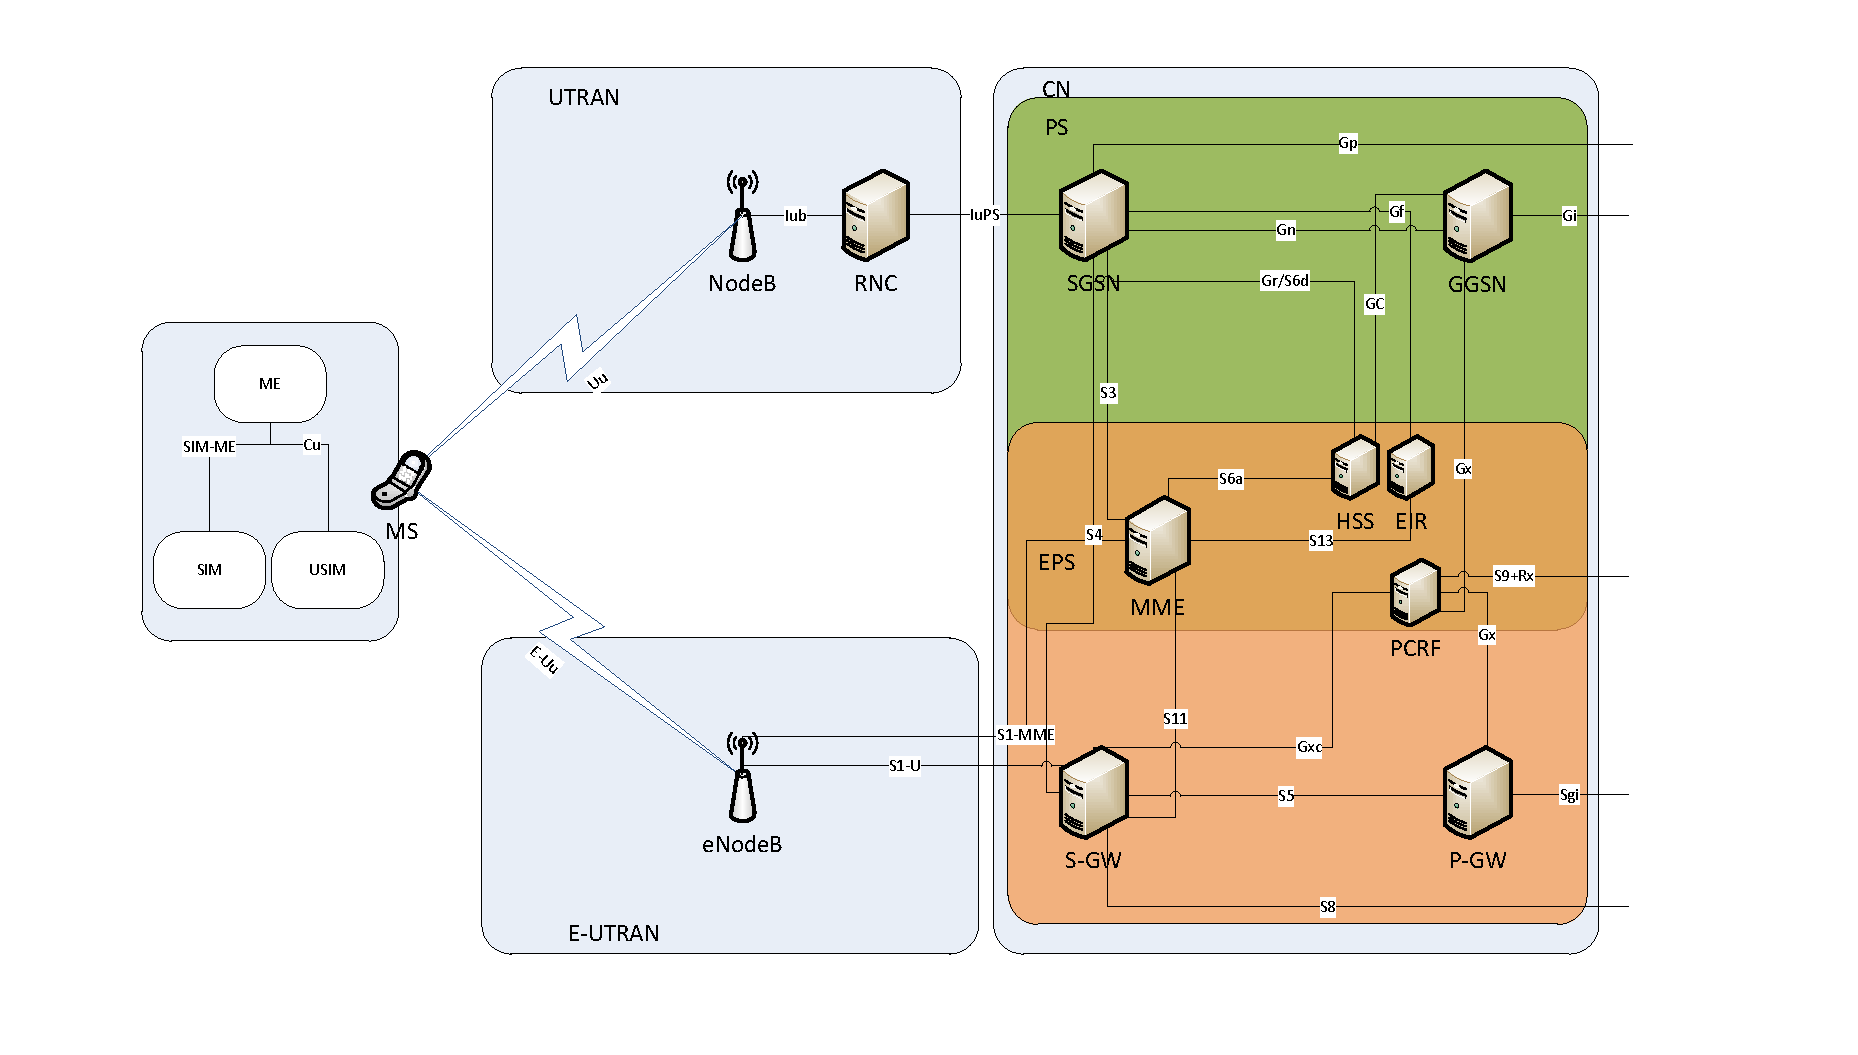
\includegraphics[width=1.0\textwidth]{images/3gpp/eps_ps-overview.pdf}
 \caption{Beispielnetz}\label{fig:netzwerk2}
\end{figure}

List of interfaces in the 3G/LTE PS network
\begin{itemize}
\item \textbf{Uu}: Interface between the mobile station (MS) and the fixed network part in Iu mode. The Uu interface is the Iu mode network interface for providing packet data services over the radio to the MS. The MT part of the MS is used to access the UMTS services through this interface.
\item \textbf{Iub}: Interface between a NodeB and a RNC.
\item \textbf{IuPS}: Interface between a RNC and a SGSN.

\item \textbf{S1-U}: Interface between a eNodeB and a S-GW. User plane bearer tunneling.
\item \textbf{S1-MME}: Interface between a eNodeB and a MME.
\item \textbf{S3}: Interface between a SGSN and a MME. User/bearer information exchange for active/idle state 3g network access mobility.
\item \textbf{S4}: Interface between a SGSN and a S-GW.	 2G user plane tunneling. GPRS mobility and control.
\item \textbf{S5}: Interface between a S-GW and a P-GW within the same PLMN. User plane tunneling; S-GW relocation due to mobility.
\item \textbf{S6a}: Interface between a MME and a HSS. Auth/auth data transfer to evolved system.
\item \textbf{Gr/S6d}: Interface between a SGSN and a HSS. 
\item \textbf{S8}: Interface between a S-GW and a P-GW in different PLMNs. Inter-PLMN variant to S5.
\item \textbf{S9}: Interface between a PRCF and the packet data network. Data exchange to visited PCRF PLMN.
\item \textbf{S11}: Interface between a S-GW and a MME.
\item \textbf{S12}: UTRAN to S-GW reference point. Based on Iu-u/Gn-u. Direct Tunnel via GTP-U.
\item \textbf{S13}: Interface between a MME and a EIR. UE identity check.
\item \textbf{SGi}: The reference point between the EPC based PLMN and the packet data network. Same as Gi for 3gpp.

\item \textbf{GC}: Interface between a HSS and a GGSN.
\item \textbf{Gf}: Interface between a SGSN and a EIR.
\item \textbf{Gi}: Reference point between Packet Domain and an external packet data network.
\item \textbf{Gn}: Interface between two GSNs within the same PLMN.
\item \textbf{Gp}: Interface between two GSNs in different PLMNs. The Gp interface allows support of Packet Domain network services across areas served by the co-operating PLMNs.
\item \textbf{Gx}: Interface between a PCRF and a P-GW/GGSN. QoS policy and charging rules transfer.
\item \textbf{Gxc}: Interface between a PCRF and a S-GW.

\item \textbf{Rx}: Interface between a PRCF and the packet data network.
\end{itemize}

\section{Control Plane Protocol Stacks}

\begin{figure}[htbp]
 \centering
 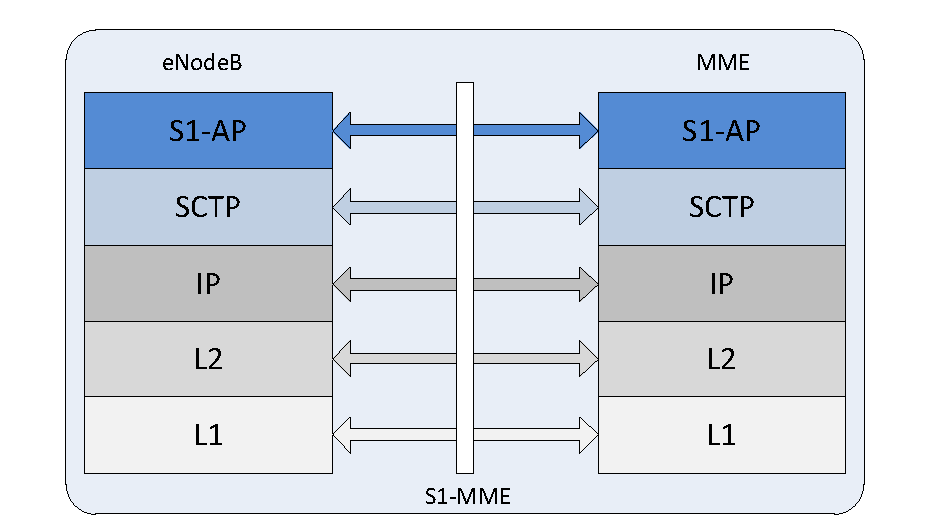
\includegraphics[width=1.0\textwidth]{images/3gpp/eNB-MME-layers.pdf}
 \caption{Beispielnetz}\label{fig:3gpp-enbmme}
\end{figure}

\begin{figure}[htbp]
 \centering
 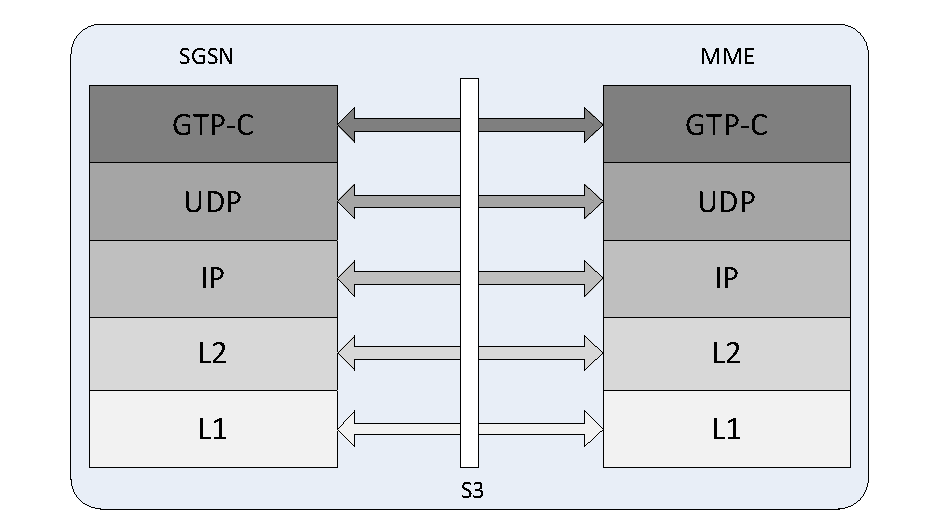
\includegraphics[width=1.0\textwidth]{images/3gpp/SGSN-MME-layers.pdf}
 \caption{Beispielnetz}\label{fig:3gpp-sgsnmme}
\end{figure}

\begin{figure}[htbp]
 \centering
 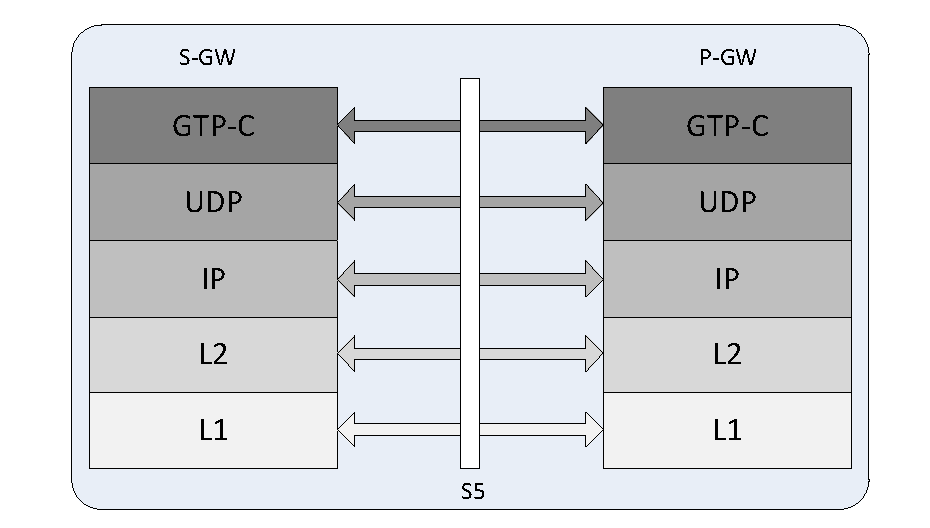
\includegraphics[width=1.0\textwidth]{images/3gpp/S-GW-P-GW-layers.pdf}
 \caption{Beispielnetz}\label{fig:3gpp-sgwpgw}
\end{figure}

\begin{figure}[htbp]
 \centering
 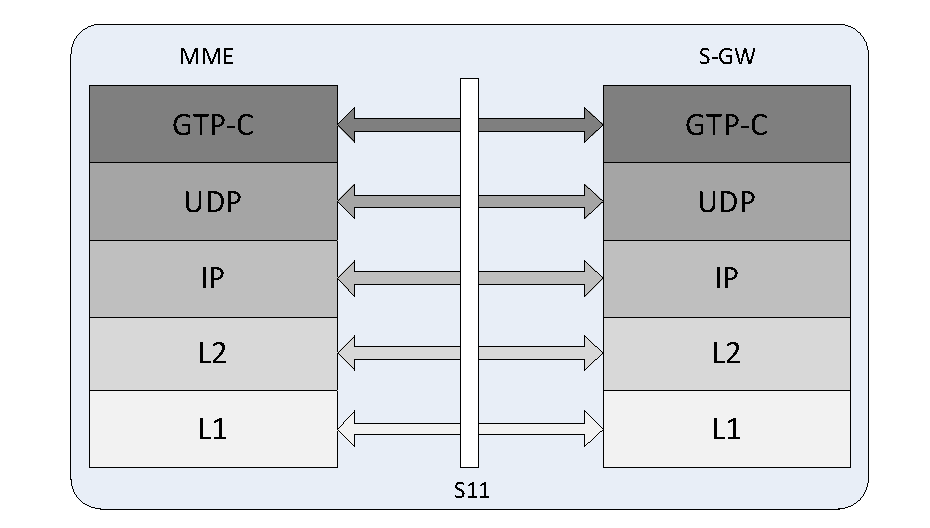
\includegraphics[width=1.0\textwidth]{images/3gpp/MME-S-GW-layers.pdf}
 \caption{Beispielnetz}\label{fig:3gpp-mmesgw}
\end{figure}


\begin{figure}[htbp]
 \centering
 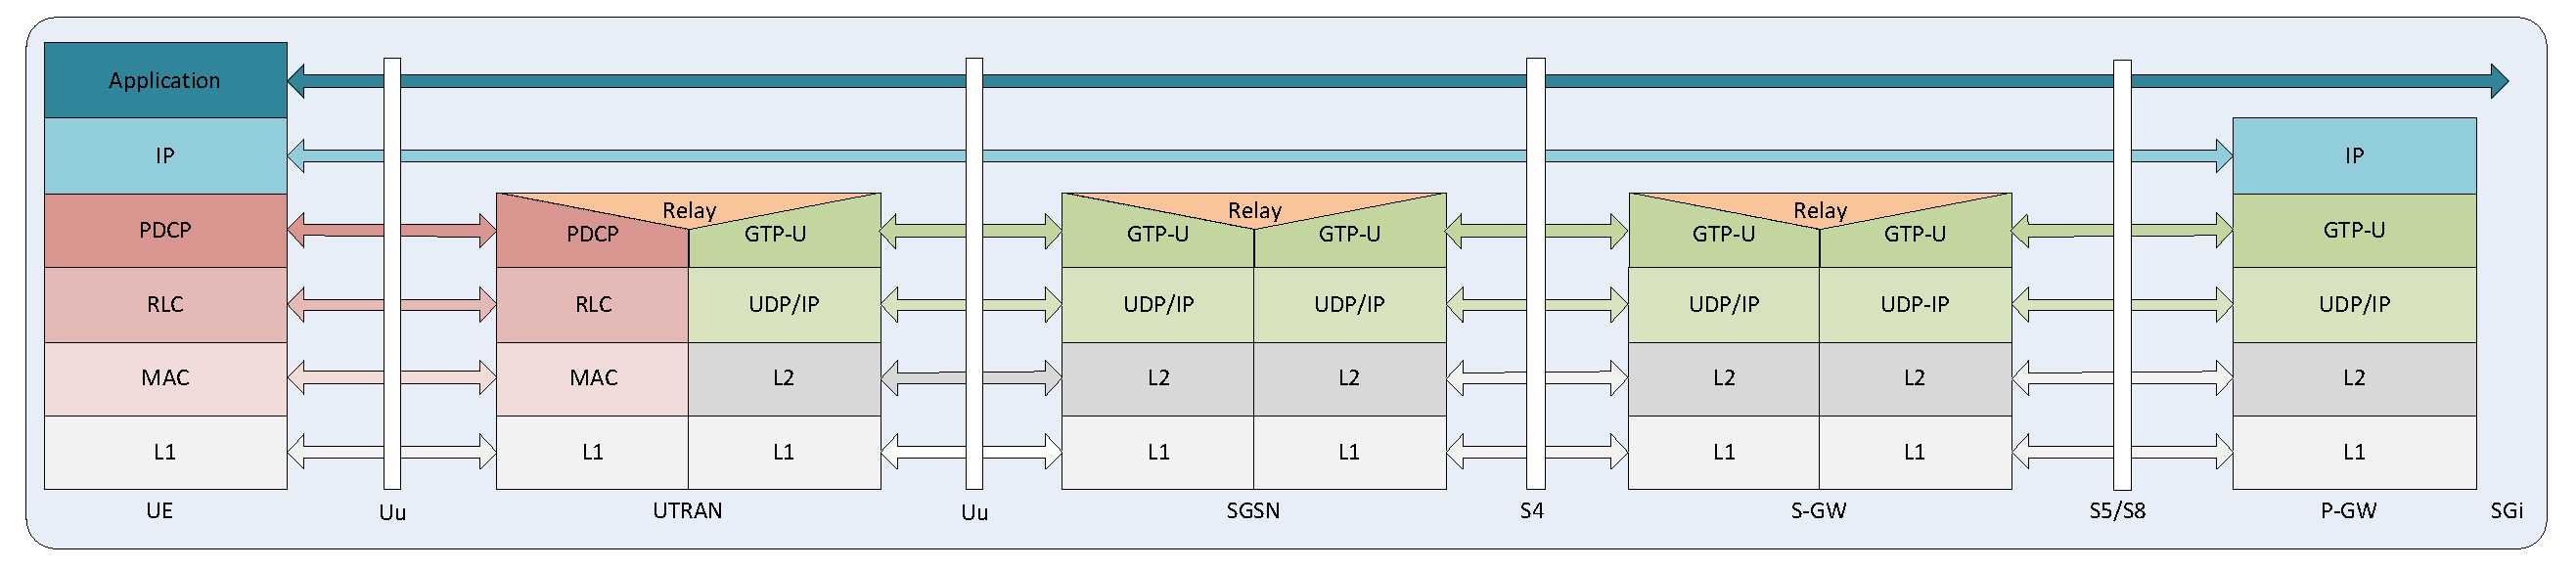
\includegraphics[width=1.0\textwidth]{images/3gpp/3g-userplane.pdf}
 \caption{Beispielnetz}\label{fig:3gpp-umtsuserplane}
\end{figure}

\begin{figure}[htbp]
 \centering
 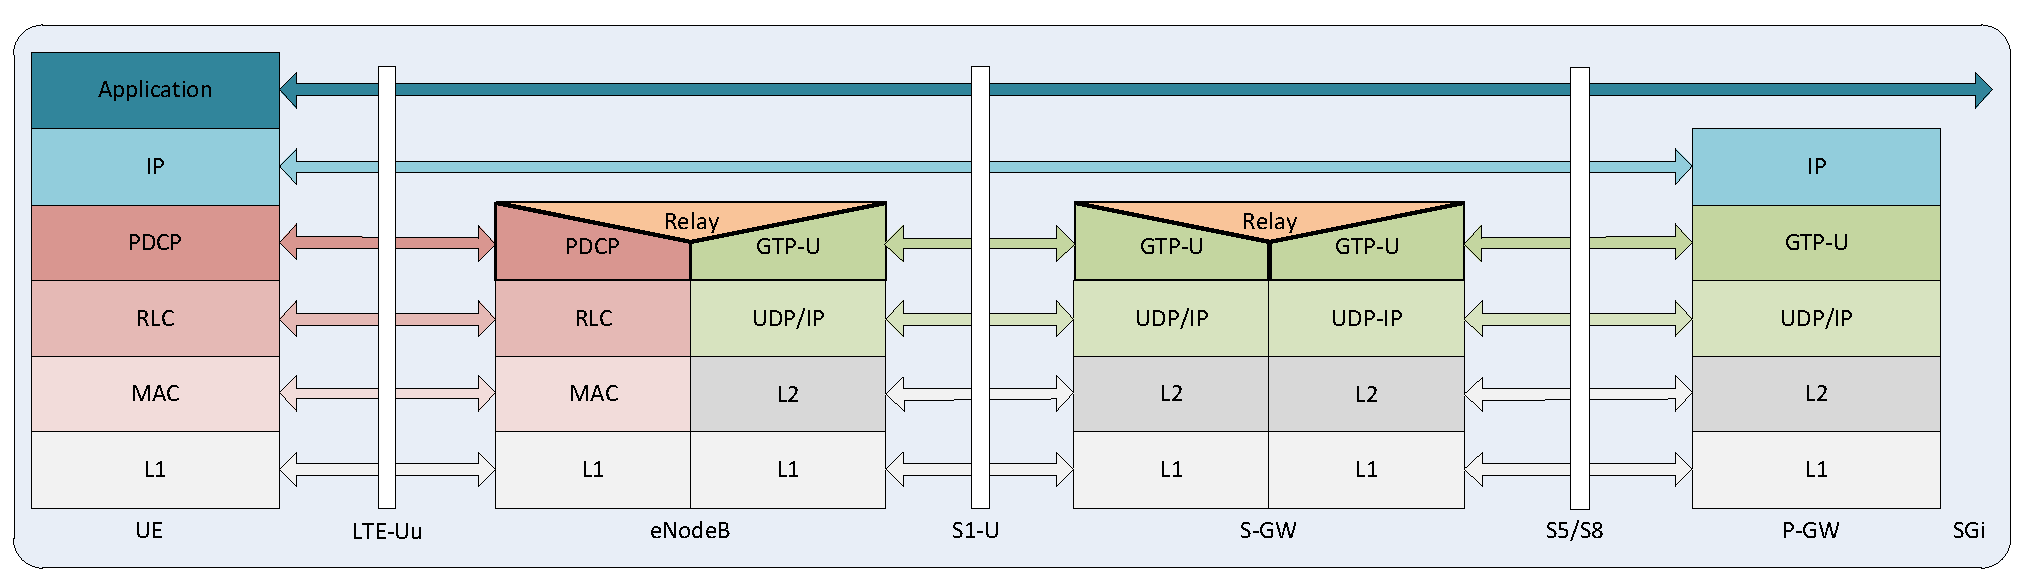
\includegraphics[width=1.0\textwidth]{images/3gpp/LTE-userplane.pdf}
 \caption{Beispielnetz}\label{fig:3gpp-lteuserplane}
\end{figure}


\section{Bearers}

As you said only 11 bearer are permitted.
So PDN connection(Default bearer) + Dedicated bearers put together should not exceed 11 bearers at any instant of time at UE side.
Theoretically 11 PDN connections are possible. But i dont think it will be of any use in practical EPS topology.

One UE Can have Maximum 3 PDN connection.
where as my knowledge is concern one UE can support maximum 11 bearers, 3 default and 8 dedicated bearers.

Does I will get in any spec for this. As the default bearer are of  NON-GBR type and and there are 5-9 are of NON-GBR QCI so I think a ue can have maximum 5 default bearer If two default bearer can not use same QCI.

\begin{figure}[htbp]
 \centering
 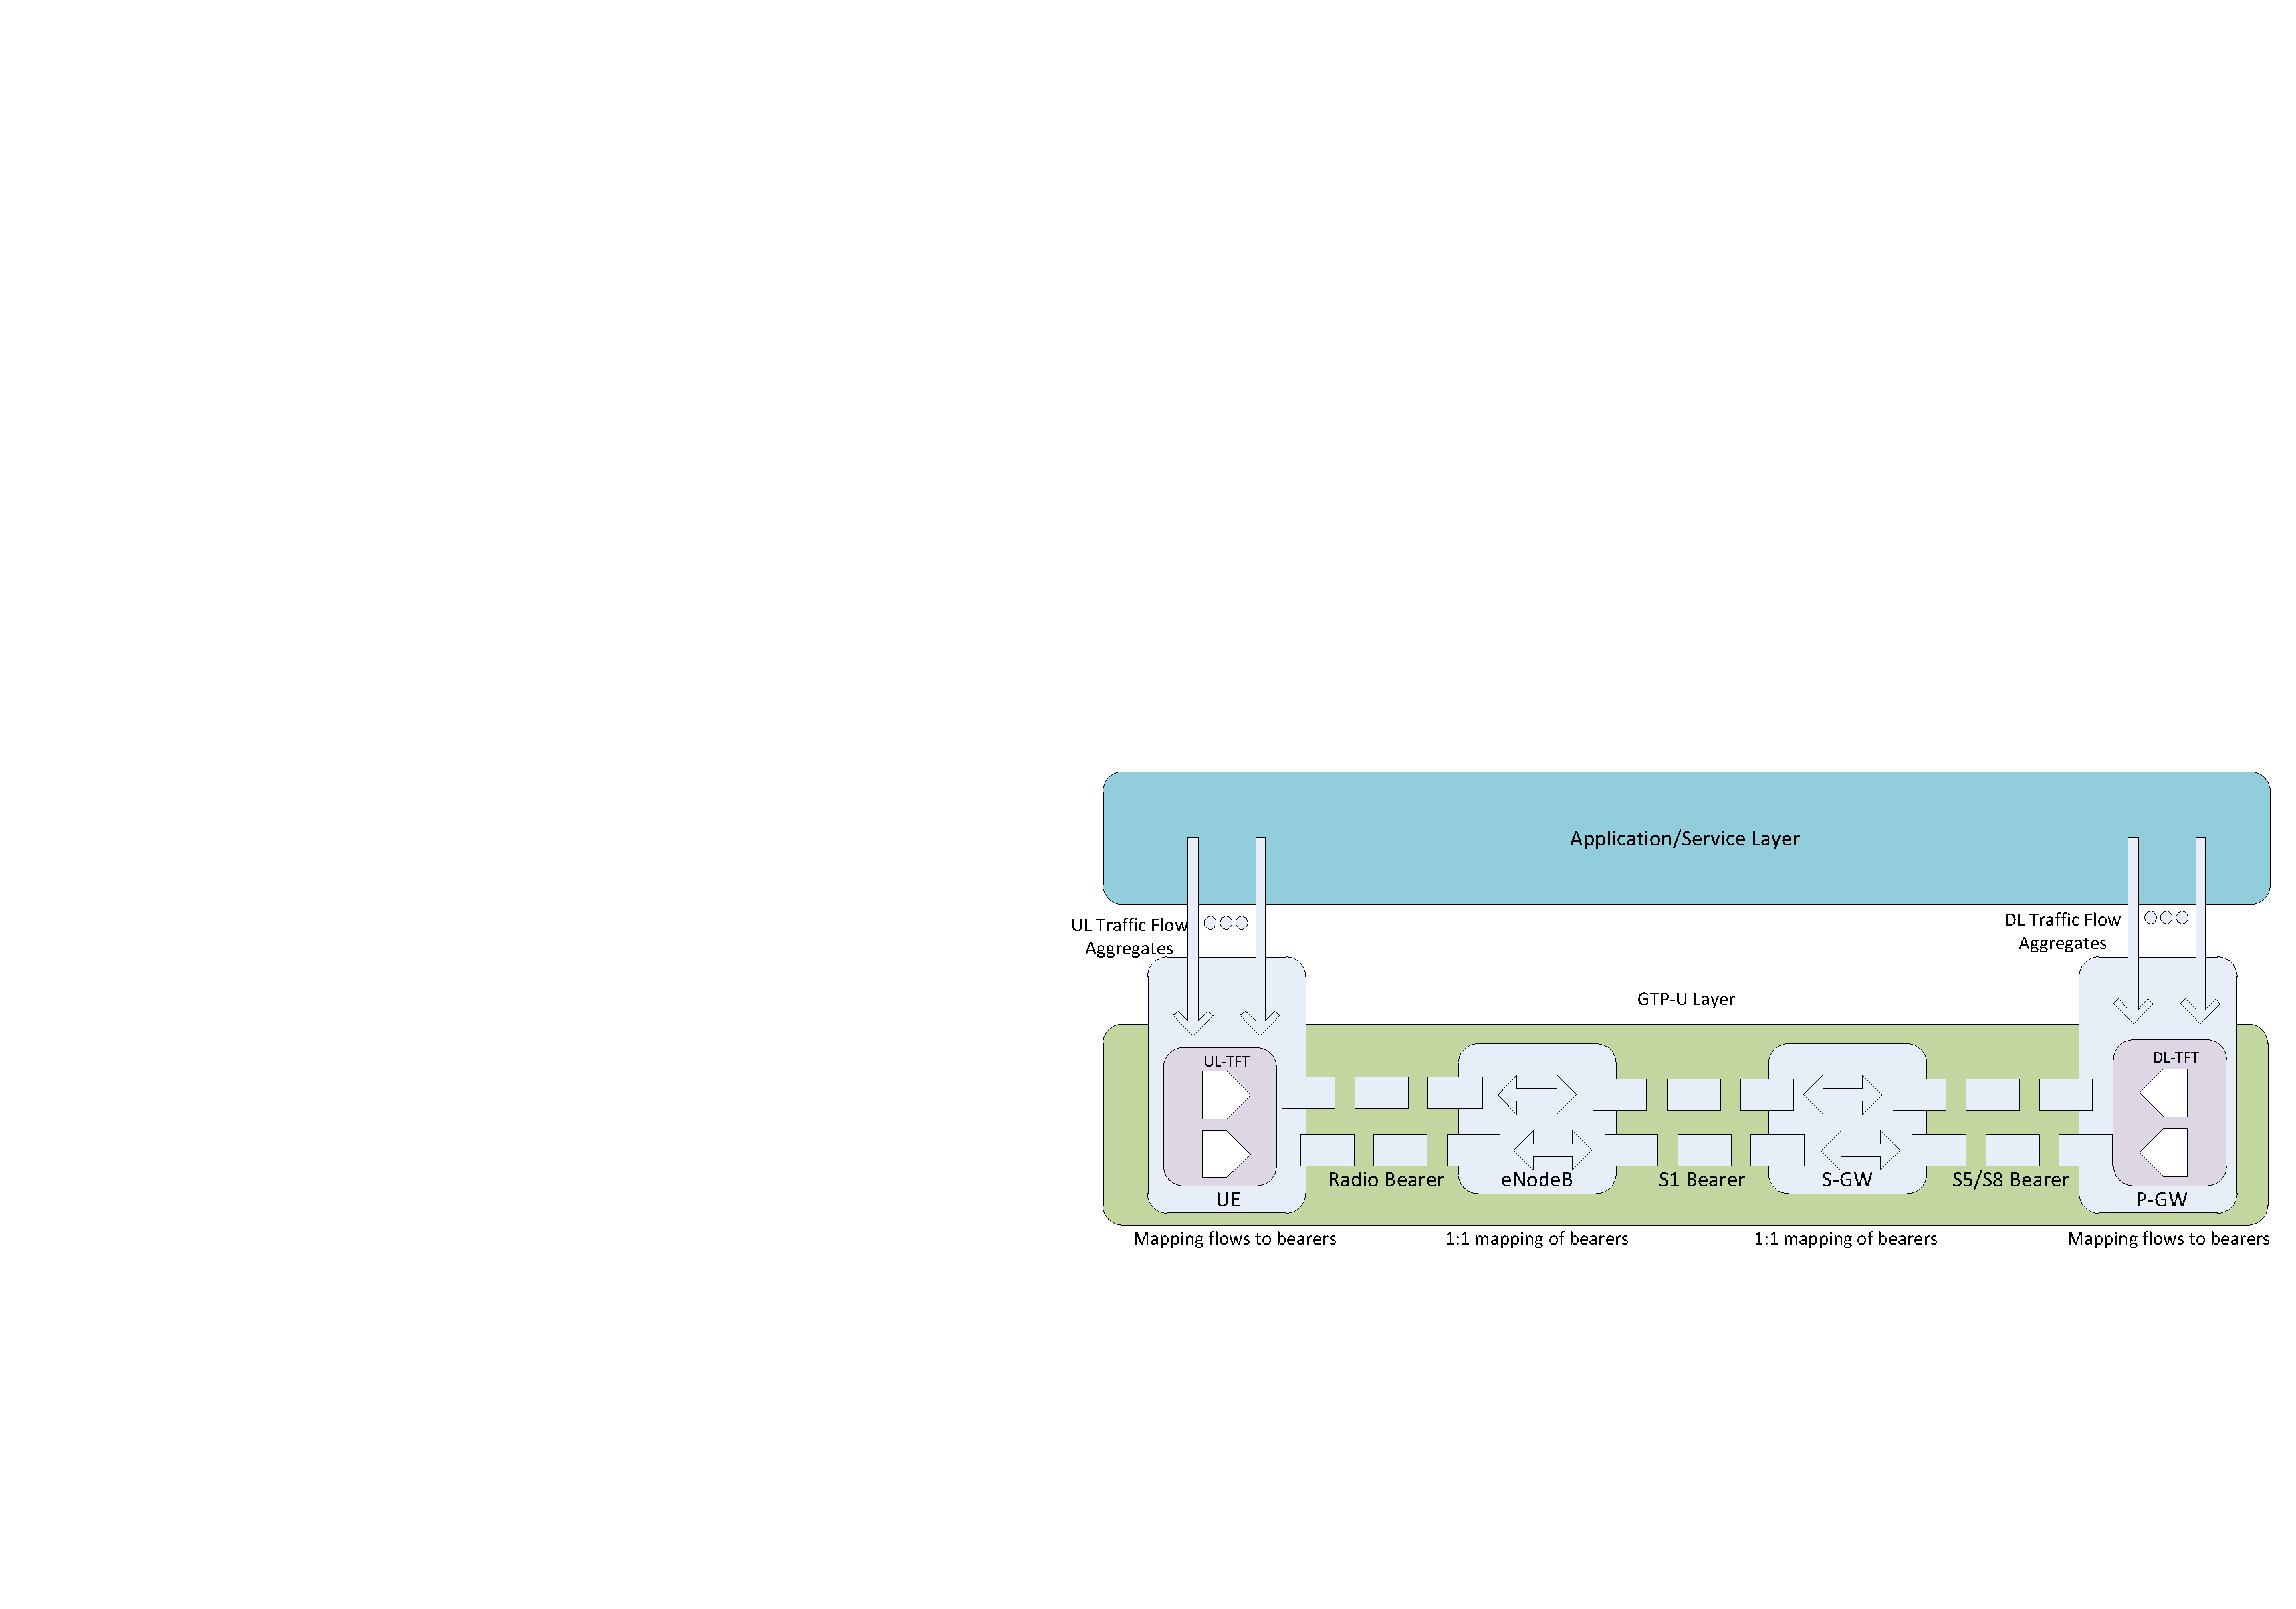
\includegraphics[width=1.0\textwidth]{images/3gpp/bearers.pdf}
 \caption{Beispielnetz}\label{fig:3gpp-bearers}
\end{figure}


\begin{figure}[htbp]
 \centering
 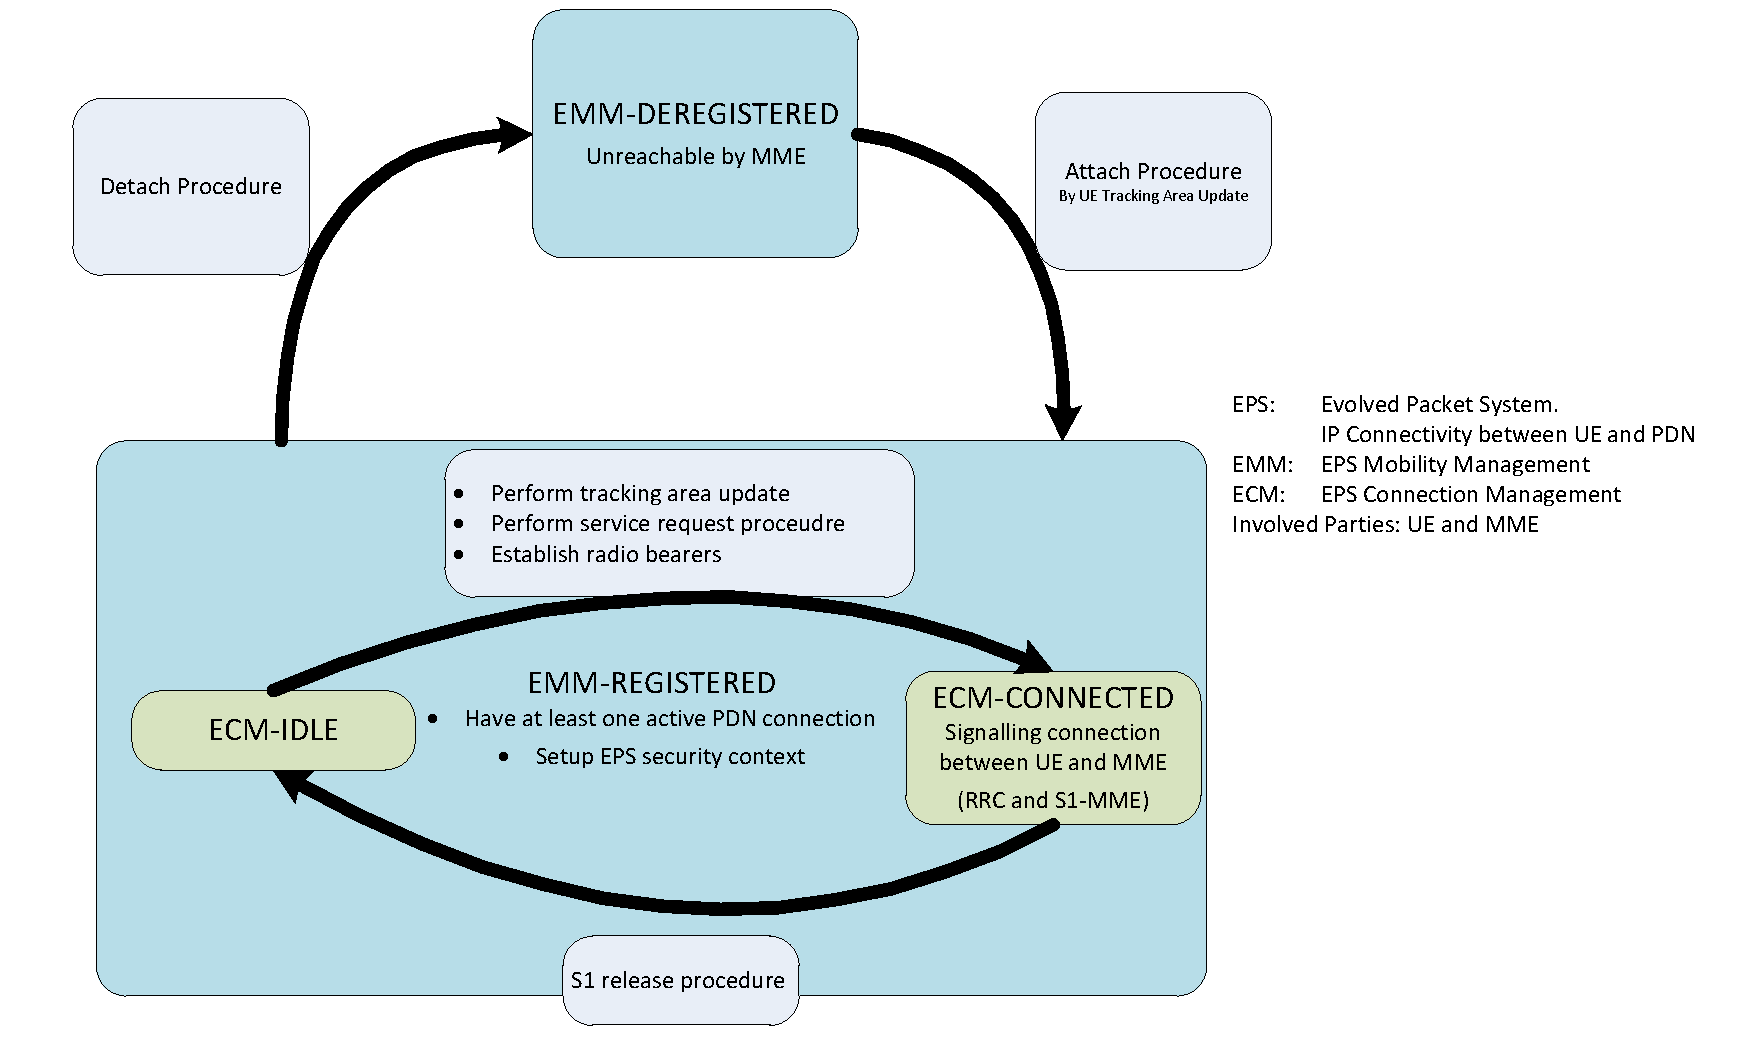
\includegraphics[width=1.0\textwidth]{images/3gpp/ECM-states.pdf}
 \caption{Beispielnetz}\label{fig:3gpp-ecmstates}
\end{figure}

\begin{itemize}
\item 	Every bearer has a predefined QoS level between UE and P-GW.
		==> Level of Granularity for QoS control.
\item	Initial bearer QoS level assigned by network based on subscription data.
\item	Guaranteed Bit Rate (GBR) bearers: dedicated network resources permanently allocated at est/mod. Otherwise Non-GBR.
\item	The Traffic Flow Template (TFT) belonging to a bearer is a set of packet filters that assign traffic flows to the bearer.
\item	UL-TFT at UE, DL-TFT at PCEF (P-GW).
\item 	default bearer: always-on IP connectivity for the UE to a PDN
\item	dedicated bearer:   
			\begin{itemize}
				\item any additional bearer for the same PDN
				\item Traffic Flow Template (TFT) associated with every ded. bearer
				\item establishment/modification decision only by EPC
				\item QoS level assignment only by EPC
			\end{itemize}

\item	default bearer may be used as {m,c}atch-all traffic bearer for everything that does not match any filter
\item	Every bearer associated with QCI and ARP.

QoS class identifier (QCI): standardized scalar as reference for node-specific QoS parameters
Allocation and Retention Policy (ARP): priority level preemption capability, preemption vulnerability.

\item	All simultaneously active bearers by one UE are provided are provided by the same P-GW.
\end{itemize}

EMM Service request procedure

\begin{figure}[htbp]
 \centering
 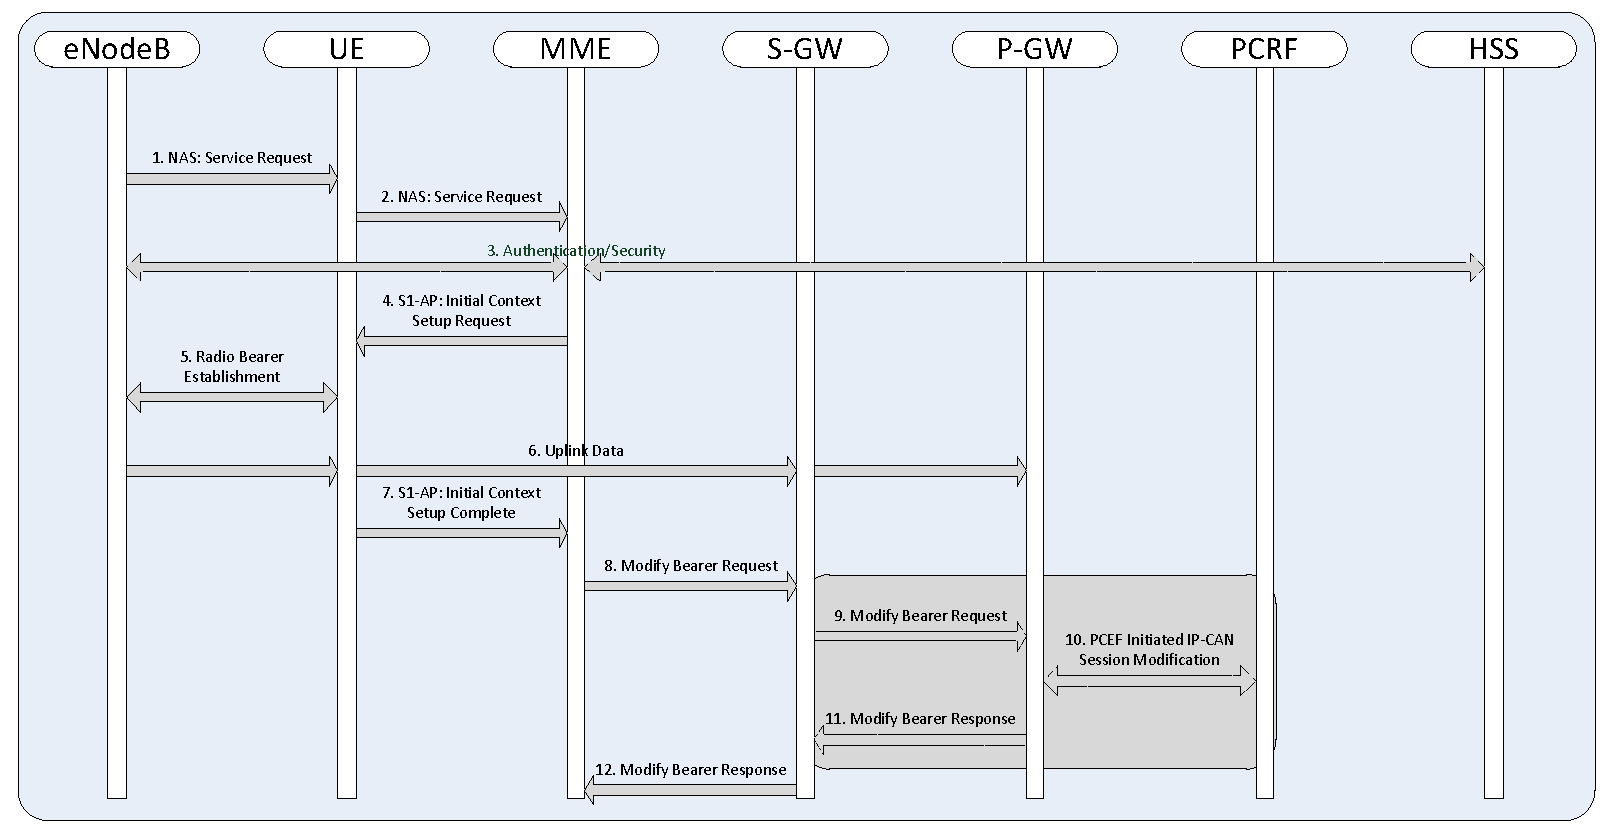
\includegraphics[width=1.0\textwidth]{images/3gpp/UE-service-request.pdf}
 \caption{Beispielnetz}\label{fig:3gpp-ueservicereq}
\end{figure}

Annotations:
1. Encapsulated in RRC message.
2. Forwarded in S1-AP Initial UE Message.
3. Various security procedures.


\section{Information Storage}
per PLMN node, cf. 3GPP TS 23.401 clause 5.7.

\begin{figure}[htbp]
 \centering
 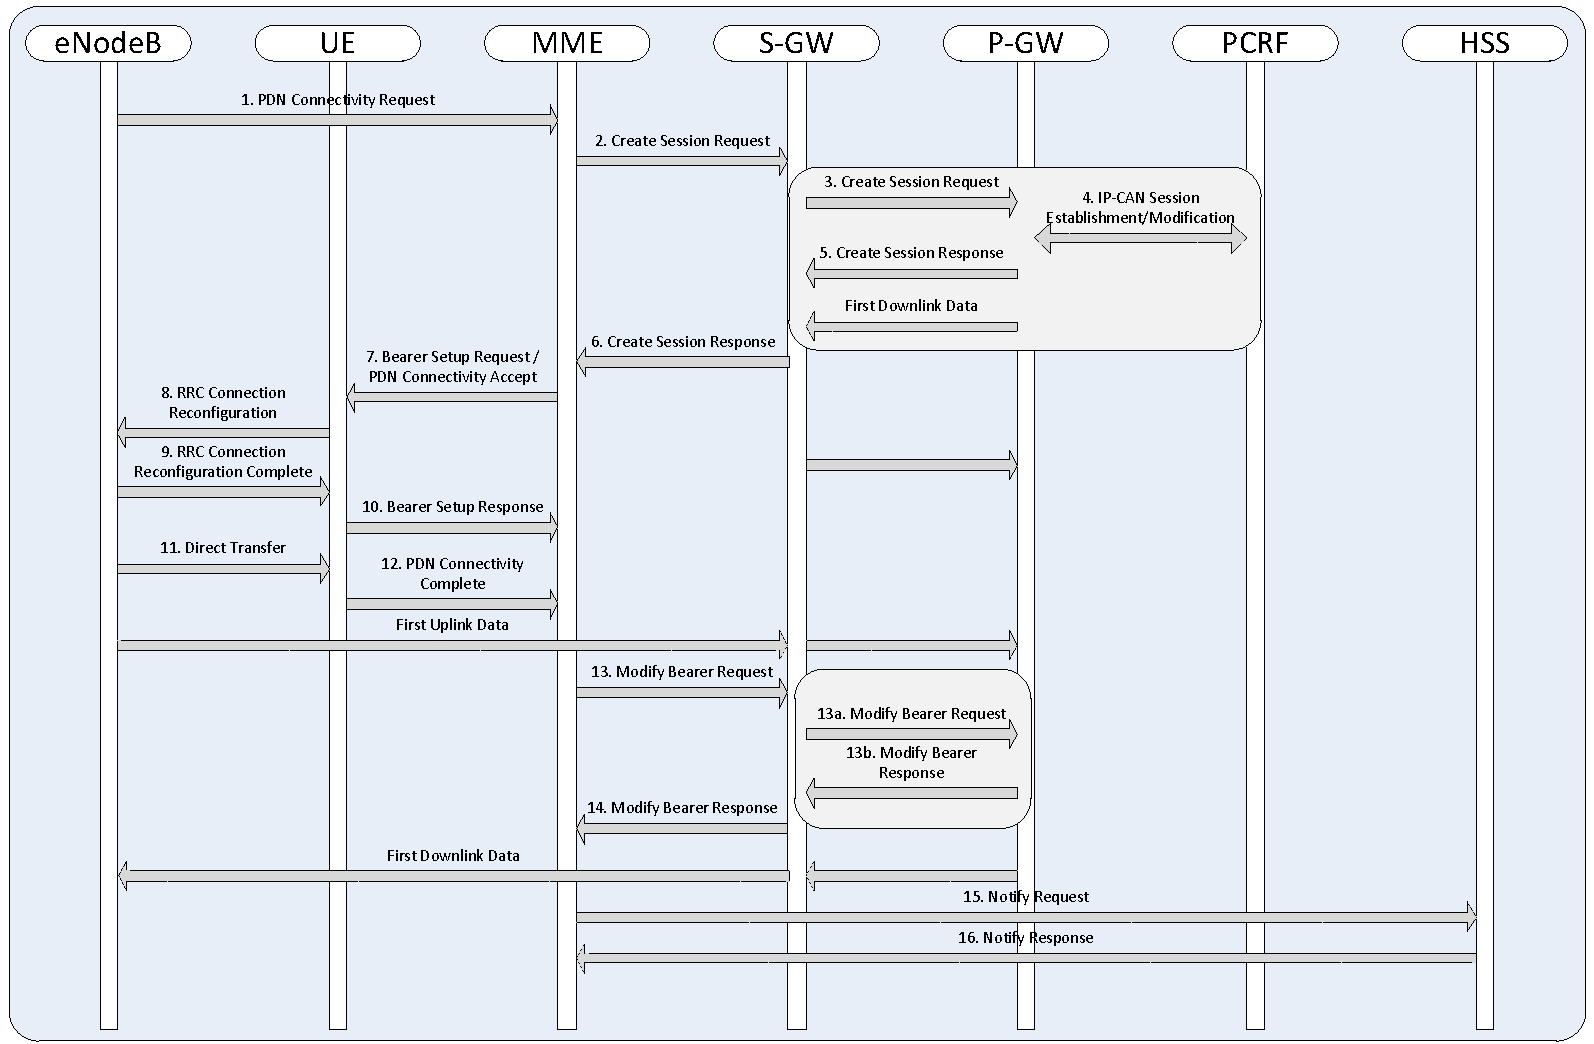
\includegraphics[width=1.0\textwidth]{images/3gpp/UE-requested-PDN-connectivity.pdf}
 \caption{Beispielnetz}\label{fig:3gpp-uepdnreq}
\end{figure}


\section{GTP}
\subsection{GTPv2}



\begin{tabular}{c|c|c|c|c|c|c|c|c|}
\multicolumn{1}{c}{} & \multicolumn{8}{c}{\textbf{Bits}} \\
\cline{2-9} \textbf{Octets} & 8 & 7 & 6 & 5 & 4 & 3 & 2 & 1 \\ 
\cline{2-9} 1 & \multicolumn{3}{c|}{Version}  & P & T & Spare & Spare & Spare \\ 
\cline{2-9} 2 & \multicolumn{8}{c|}{Message Type}  \\ 
\cline{2-9} 3 & \multicolumn{8}{c|}{Message Length (1st Octet)}  \\ 
\cline{2-9} 4 & \multicolumn{8}{c|}{Message Length (2nd Octet)}  \\ 
\cline{2-9} m to & \multicolumn{8}{c|}{\multirow{2}{10cm}{If T flag is set to 1, then TEID shall be placed into octets 5-8. Otherwise, TEID field is not present at all.}} \\ 
 k(m+3) & \multicolumn{8}{c|}{} \\ 
\cline{2-9} n to (n+2) & \multicolumn{8}{c|}{Sequence Number} \\ 
\cline{2-9} (n+3) & \multicolumn{8}{c|}{Spare} \\ 
\cline{2-9} 
\end{tabular} 
\subsection{GTP-C}

\begin{tabular}{c|c|c|c|c|c|c|c|c|}
\multicolumn{1}{c}{} & \multicolumn{8}{c}{\textbf{Bits}} \\
\cline{2-9} \textbf{Octets} & 8 & 7 & 6 & 5 & 4 & 3 & 2 & 1 \\ 
\cline{2-9} 1 & \multicolumn{3}{c|}{Version}  & P & T=1 & Spare & Spare & Spare \\ 
\cline{2-9} 2 & \multicolumn{8}{c|}{Message Type}  \\ 
\cline{2-9} 3 & \multicolumn{8}{c|}{Message Length (1st Octet)}  \\ 
\cline{2-9} 4 & \multicolumn{8}{c|}{Message Length (2nd Octet)}  \\ 
\cline{2-9} 5 & \multicolumn{8}{c|}{Tunnel Endpoint Identifier (1st Octet)} \\ 
\cline{2-9} 6 & \multicolumn{8}{c|}{Tunnel Endpoint Identifier (2nd Octet)} \\ 
\cline{2-9} 7 & \multicolumn{8}{c|}{Tunnel Endpoint Identifier (3rd Octet)} \\ 
\cline{2-9} 8 & \multicolumn{8}{c|}{Tunnel Endpoint Identifier (4th Octet)} \\ 
\cline{2-9} 9 & \multicolumn{8}{c|}{Sequence Number (1st Octet)} \\
\cline{2-9} 10 & \multicolumn{8}{c|}{Sequence Number (2nd Octet)} \\
\cline{2-9} 11 & \multicolumn{8}{c|}{Sequence Number (3rd Octet)} \\
\cline{2-9} 12 & \multicolumn{8}{c|}{Spare} \\
\cline{2-9}
\end{tabular} 

12 Byte GTPv2-C header.

\subsubsection{Create Session Request Message}

Information Elements Table for PDP Context Activation Case only

\begin{longtabu}{|p{2cm}|c|p{1.5cm}|p{8cm}|}
\hline
Information Element 						& IE Type 					& Max Wire Size (Bytes)	& Comment \\ \hline
IMSI 										& IMSI 						& 12					& \\ \hline
MSISDN 										& MSISDN					& 12					& On S11 Interface if provided by HSS; In case of UE requested connectivity if MME has it stored. \\ \hline
MEI Identity 								& MEI 						& 12					& If available at MME. \\ \hline
User Location Information 					& ULI						& 						& E-UTRAN initial attach \&  UE requested connectivity only; included by S-GW if received from MME via S5/S8; included on S4 and S5/S8 for PDP context activation, either CGI, SAI, or RAI. \\ \hline
Serving Network								& Serving Network			& 						& Initial E-UTRAN attach, context activation and UE requested connectivity \\ \hline
RAT Type									& RAT Type					& 5						& \\ \hline
Indication Flags							& Indication				& 6						& Flags: S5/S8 Protocol Type; Dual Address Bearer Flag; Handover Indication; Direct Tunnel Flag; Piggybacking Supported; Change Reporting Support Indication \\ \hline
Sender F-TEID for Control Plane				& F-TEID					& 						& \\ \hline
P-G S5/S8 Address for Control Plane or PMIP	& F-TEID					& 						& On S11/S4 interfaces; 0 if initial attach, context activation or PDN connectivity \\ \hline
Access Point Name							& APN						& 83					& \\ \hline
Selection Mode								& Selection Mode			& 						& Indicate whether subscribed or non-subscribed, chosen by MME, was selected \\ \hline
PDN Type									& PDN Type					& 						& IPv4, IPv6 or IPv4v6. \\ \hline
PDN Address Allocation						& PAA						& 26					& Set to static IP address; else (dynamic) to 0.0.0.0 or IPv6 Prefix Length 0. \\ \hline
Maximum APN Restriction						& APN Restriction			& 						& Set to most stringent restriction of any active bearer. \\ \hline
Aggregate Maximum Bit Rate					& ABMR						& 12					& \\ \hline
Protocol Configuration Options				& PCO						& 254					& Forwarded from UE to P-GW via S-GW via MME. \\ \hline
Bearer Contexts to be created				& Bearer Context			& 						& present multiple times to represent list of bearers \\ \hline
Trace Information							& Trace Information 		& 						& If S-GW / P-GW is activated. \\ \hline
Recovery									& Recovery					& 5						& If peer node contacted for the first time. \\ \hline
MME-FQ-CSID									& FQ-CSID					& 						& Included by MME on S11 \\ \hline
SGW-FQ-CSID									& FQ-CSID					& 						& Included by S-GW on S5/S8 \\ \hline
UE Time Zone								& UE Time Zone 				& 						& Can be included by MME on S11; forwarded to P-GW via S-GW \\ \hline
User CSG Information						& UCI						& 						& If UE accessed via CSG cell or hybrid cell \\ \hline
Charging Characteristics					& Charging Characteristics	&						& \\ \hline
Private Extensions							& Private Extensions		&						& \\ \hline

\end{longtabu}

\subsubsection{Information Elements Wire Format}

\paragraph{IMSI}

\begin{tabular}{c|p{1cm}|p{1cm}|p{1cm}|p{1cm}|p{1cm}|p{1cm}|p{1cm}|p{1cm}|}
\multicolumn{1}{c}{} & \multicolumn{8}{c}{\textbf{Bits}} \\
\cline{2-9} \textbf{Octets} & 8 & 7 & 6 & 5 & 4 & 3 & 2 & 1 \\ 
\cline{2-9} 1 & \multicolumn{8}{c|}{Type = 1 (decimal)} \\ 
\cline{2-9} 2 to 3 & \multicolumn{8}{c|}{Length = n}  \\ 
\cline{2-9} 4 & \multicolumn{4}{c|}{Spare} & \multicolumn{4}{c|}{Instance} \\ 
\cline{2-9} 5 & \multicolumn{4}{c|}{Number digit 2} & \multicolumn{4}{c|}{Number digit 1} \\ 
\cline{2-9} 6 & \multicolumn{4}{c|}{Number digit 4} & \multicolumn{4}{c|}{Number digit 3} \\ 
\cline{2-9} ... & \multicolumn{4}{c|}{...} & \multicolumn{4}{c|}{...} \\ 
\cline{2-9} n+4 & \multicolumn{4}{c|}{Number digit m} & \multicolumn{4}{c|}{Number digit m-1} \\ 
\cline{2-9}
\end{tabular} 

Decimals coded as TBCD; if odd number fill last nibble with 1; max digits is 15.\\
Max IE size 12 Byte.

\paragraph{APN}

\begin{tabular}{c|p{1cm}|p{1cm}|p{1cm}|p{1cm}|p{1cm}|p{1cm}|p{1cm}|p{1cm}|}
\multicolumn{1}{c}{} & \multicolumn{8}{c}{\textbf{Bits}} \\
\cline{2-9} \textbf{Octets} & 8 & 7 & 6 & 5 & 4 & 3 & 2 & 1 \\ 
\cline{2-9} 1 & \multicolumn{8}{c|}{Type = 71 (decimal)} \\ 
\cline{2-9} 2 to 3 & \multicolumn{8}{c|}{Length = n}  \\ 
\cline{2-9} 4 & \multicolumn{4}{c|}{Spare} & \multicolumn{4}{c|}{Instance} \\ 
\cline{2-9} 5 to (n+4) & \multicolumn{8}{c|}{Access Point Name} \\ 
\cline{2-9}
\end{tabular} 

Full APN name including APN Network Identifier and APN Operator Identifier.
Network Identifier: max length 63 bytes.
Operator Identifier: mnc<3digits>.mcc<3digits>.gprs; 16 bytes (18 incl dots).
(Ex: ggsn-cluster-A.provinceB.mnc012.mcc345.gprs)

Max total $4+63+16=83$

\paragraph{AMBR}

\begin{tabular}{c|p{1cm}|p{1cm}|p{1cm}|p{1cm}|p{1cm}|p{1cm}|p{1cm}|p{1cm}|}
\multicolumn{1}{c}{} & \multicolumn{8}{c}{\textbf{Bits}} \\
\cline{2-9} \textbf{Octets} & 8 & 7 & 6 & 5 & 4 & 3 & 2 & 1 \\ 
\cline{2-9} 1 & \multicolumn{8}{c|}{Type = 72 (decimal)} \\ 
\cline{2-9} 2 to 3 & \multicolumn{8}{c|}{Length = n}  \\ 
\cline{2-9} 4 & \multicolumn{4}{c|}{Spare} & \multicolumn{4}{c|}{Instance} \\ 
\cline{2-9} 5 to 8 & \multicolumn{8}{c|}{APN-AMBR for uplink} \\ 
\cline{2-9} 9 to 12 & \multicolumn{8}{c|}{APN-AMBR for downlink} \\ 
\cline{2-9}
\end{tabular} 


Total size 12 bytes.


\paragraph{Recovery}

\begin{tabular}{c|p{1cm}|p{1cm}|p{1cm}|p{1cm}|p{1cm}|p{1cm}|p{1cm}|p{1cm}|}
\multicolumn{1}{c}{} & \multicolumn{8}{c}{\textbf{Bits}} \\
\cline{2-9} \textbf{Octets} & 8 & 7 & 6 & 5 & 4 & 3 & 2 & 1 \\ 
\cline{2-9} 1 & \multicolumn{8}{c|}{Type = 3 (decimal)} \\ 
\cline{2-9} 2 to 3 & \multicolumn{8}{c|}{Length = n}  \\ 
\cline{2-9} 4 & \multicolumn{4}{c|}{Spare} & \multicolumn{4}{c|}{Instance} \\ 
\cline{2-9} 5 to (n+4) & \multicolumn{8}{c|}{Recovery (Restart Counter} \\ 
\cline{2-9}
\end{tabular} 

IN GTPv2 first release IE length is 5 bytes. May be longer in the future.


\paragraph{MEI}

\begin{tabular}{c|p{1cm}|p{1cm}|p{1cm}|p{1cm}|p{1cm}|p{1cm}|p{1cm}|p{1cm}|}
\multicolumn{1}{c}{} & \multicolumn{8}{c}{\textbf{Bits}} \\
\cline{2-9} \textbf{Octets} & 8 & 7 & 6 & 5 & 4 & 3 & 2 & 1 \\ 
\cline{2-9} 1 & \multicolumn{8}{c|}{Type = 75 (decimal)} \\ 
\cline{2-9} 2 to 3 & \multicolumn{8}{c|}{Length = n}  \\ 
\cline{2-9} 4 & \multicolumn{4}{c|}{Spare} & \multicolumn{4}{c|}{Instance} \\ 
\cline{2-9} 5 to (n+4) & \multicolumn{8}{c|}{Mobile Equipment (ME) Identity} \\ 
\cline{2-9}
\end{tabular} 

15 (IMEI) or 16 (IMEISV) BCD digits filled with 1 to full octet. Size is 12 bytes.

\paragraph{MSISDN}

\begin{tabular}{c|p{1cm}|p{1cm}|p{1cm}|p{1cm}|p{1cm}|p{1cm}|p{1cm}|p{1cm}|}
\multicolumn{1}{c}{} & \multicolumn{8}{c}{\textbf{Bits}} \\
\cline{2-9} \textbf{Octets} & 8 & 7 & 6 & 5 & 4 & 3 & 2 & 1 \\ 
\cline{2-9} 1 & \multicolumn{8}{c|}{Type = 76 (decimal)} \\ 
\cline{2-9} 2 to 3 & \multicolumn{8}{c|}{Length = n}  \\ 
\cline{2-9} 4 & \multicolumn{4}{c|}{Spare} & \multicolumn{4}{c|}{Instance} \\ 
\cline{2-9} 5 & \multicolumn{4}{c|}{Number digit 2} & \multicolumn{4}{c|}{Number digit 1} \\ 
\cline{2-9} 6 & \multicolumn{4}{c|}{Number digit 4} & \multicolumn{4}{c|}{Number digit 3} \\ 
\cline{2-9} ... & \multicolumn{4}{c|}{...} & \multicolumn{4}{c|}{...} \\ 
\cline{2-9} n+4 & \multicolumn{4}{c|}{Number digit m} & \multicolumn{4}{c|}{Number digit m-1} \\ 
\cline{2-9}
\end{tabular} 

MSISDN limited to 15 digits. Max total size 12 bytes.


\paragraph{Indication}
\centering
\begin{tabular}{c|p{1cm}|p{1cm}|p{1cm}|p{1cm}|p{1cm}|p{1cm}|p{1cm}|p{1cm}|}
\multicolumn{1}{c}{} & \multicolumn{8}{c}{\textbf{Bits}} \\
\cline{2-9} \textbf{Octets} & 8 & 7 & 6 & 5 & 4 & 3 & 2 & 1 \\ 
\cline{2-9} 1 & \multicolumn{8}{c|}{Type = 77 (decimal)} \\ 
\cline{2-9} 2 to 3 & \multicolumn{8}{c|}{Length = n}  \\ 
\cline{2-9} 4 & \multicolumn{4}{c|}{Spare} & \multicolumn{4}{c|}{Instance} \\ 
\cline{2-9} 5 & DAF & DTF & HI & DFI & OI & ISRSI & ISRAI & SGWCI \\ 
\cline{2-9} 6 & Spare & UIMSI & CFSI & CRSI & P & PT & SI & MSV \\ 
\cline{2-9} 7 to (n+4) & \multicolumn{8}{c|}{These octet(s) is/are present only if explicitly specified} \\ 
\cline{2-9}
\end{tabular} 

Size is 7 bytes.

\paragraph{PCO}
\centering
\begin{tabular}{c|p{1cm}|p{1cm}|p{1cm}|p{1cm}|p{1cm}|p{1cm}|p{1cm}|p{1cm}|}
\multicolumn{1}{c}{} & \multicolumn{8}{c}{\textbf{Bits}} \\
\cline{2-9} \textbf{Octets} & 8 & 7 & 6 & 5 & 4 & 3 & 2 & 1 \\ 
\cline{2-9} 1 & \multicolumn{8}{c|}{Type = 78 (decimal)} \\ 
\cline{2-9} 2 to 3 & \multicolumn{8}{c|}{Length = n}  \\ 
\cline{2-9} 4 & \multicolumn{4}{c|}{Spare} & \multicolumn{4}{c|}{Instance} \\ 
\cline{2-9} 5 to (n+4) & \multicolumn{8}{c|}{Protocol Configuration Options} \\
\cline{2-9}
\end{tabular} 

Minimum length 4+3-3, maximum length 4+253-3; average?


\paragraph{PAA}
\centering

\begin{tabular}{c|p{1cm}|p{1cm}|p{1cm}|p{1cm}|p{1cm}|p{1cm}|p{1cm}|p{1cm}|}
\multicolumn{1}{c}{} & \multicolumn{8}{c}{\textbf{Bits}} \\
\cline{2-9} \textbf{Octets} & 8 & 7 & 6 & 5 & 4 & 3 & 2 & 1 \\ 
\cline{2-9} 1 & \multicolumn{8}{c|}{Type = 79 (decimal)} \\ 
\cline{2-9} 2 to 3 & \multicolumn{8}{c|}{Length = n}  \\ 
\cline{2-9} 4 & \multicolumn{4}{c|}{Spare} & \multicolumn{4}{c|}{Instance} \\ 
\cline{2-9} 5 & \multicolumn{5}{c|}{Spare} & \multicolumn{3}{c|}{PDN Type} \\
\cline{2-9} 6 to (n+4) & \multicolumn{8}{c|}{PDN Adress and Prefix} \\
\cline{2-9}
\end{tabular} 

Either 9 (IPv4), 22 (IPv6), or 26 (IPv4v6).


\paragraph{RAT Type}
\centering
\begin{tabular}{c|p{1cm}|p{1cm}|p{1cm}|p{1cm}|p{1cm}|p{1cm}|p{1cm}|p{1cm}|}
\multicolumn{1}{c}{} & \multicolumn{8}{c}{\textbf{Bits}} \\
\cline{2-9} \textbf{Octets} & 8 & 7 & 6 & 5 & 4 & 3 & 2 & 1 \\ 
\cline{2-9} 1 & \multicolumn{8}{c|}{Type = 82 (decimal)} \\ 
\cline{2-9} 2 to 3 & \multicolumn{8}{c|}{Length = n}  \\ 
\cline{2-9} 4 & \multicolumn{4}{c|}{Spare} & \multicolumn{4}{c|}{Instance} \\ 
\cline{2-9} 5 & \multicolumn{8}{c|}{RAT Type} \\
\cline{2-9} 6 to (n+4) & \multicolumn{8}{c|}{These octet(s) is/are present only if explicitly specified} \\
\cline{2-9}
\end{tabular} 

Maximum length 5 to ?.

\paragraph{Serving Network}

\centering
\begin{tabular}{c|p{1cm}|p{1cm}|p{1cm}|p{1cm}|p{1cm}|p{1cm}|p{1cm}|p{1cm}|}
\multicolumn{1}{c}{} & \multicolumn{8}{c}{\textbf{Bits}} \\
\cline{2-9} \textbf{Octets} & 8 & 7 & 6 & 5 & 4 & 3 & 2 & 1 \\ 
\cline{2-9} 1 & \multicolumn{8}{c|}{Type = 83 (decimal)} \\ 
\cline{2-9} 2 to 3 & \multicolumn{8}{c|}{Length = n}  \\ 
\cline{2-9} 4 & \multicolumn{4}{c|}{Spare} & \multicolumn{4}{c|}{Instance} \\ 
\cline{2-9} 5 & \multicolumn{4}{c|}{MCC digit 2} & \multicolumn{4}{c|}{MCC digit 1} \\ 
\cline{2-9} 6 & \multicolumn{4}{c|}{MNC digit 3} & \multicolumn{4}{c|}{MCC digit 3} \\ 
\cline{2-9} 7 & \multicolumn{4}{c|}{MNC digit 2} & \multicolumn{4}{c|}{MNC digit 1} \\ 
\cline{2-9} 8 to (n+4) & \multicolumn{8}{c|}{These octet(s) is/are present only if explicitly specified} \\
\cline{2-9}
\end{tabular} 

Maximum length 7 to ?.


\paragraph{User Location Information}

\centering
\begin{tabular}{c|p{1cm}|p{1cm}|p{1cm}|p{1cm}|p{1cm}|p{1cm}|p{1cm}|p{1cm}|}
\multicolumn{1}{c}{} & \multicolumn{8}{c}{\textbf{Bits}} \\
\cline{2-9} \textbf{Octets} & 8 & 7 & 6 & 5 & 4 & 3 & 2 & 1 \\ 
\cline{2-9} 1 & \multicolumn{8}{c|}{Type = 86 (decimal)} \\ 
\cline{2-9} 2 to 3 & \multicolumn{8}{c|}{Length = n}  \\ 
\cline{2-9} 4 & \multicolumn{4}{c|}{Spare} & \multicolumn{4}{c|}{Instance} \\ 
\cline{2-9} 5 & \multicolumn{3}{c|}{Spare} & ECGI & TAI & RAI & SAI & CGI \\ 
\cline{2-9} a to a+6 & \multicolumn{8}{c|}{CGI} \\ 
\cline{2-9} 7 & \multicolumn{8}{c|}{SAI} \\ 
\cline{2-9} 7 & \multicolumn{8}{c|}{RAI} \\ 
\cline{2-9} 7 & \multicolumn{8}{c|}{TAI} \\ 
\cline{2-9} 7 & \multicolumn{8}{c|}{ECGI} \\ 
\cline{2-9} 8 to (n+4) & \multicolumn{8}{c|}{These octet(s) is/are present only if explicitly specified} \\
\cline{2-9}
\end{tabular} 


\subsection{GTP-U}




%%%%%%%%%%%%%%%%%%%%%%%%%%%%%%%%%%%%%%%%%%%%%%%%%%%%%%%%%%%%%%%%%%%%%%%%%%%%%%%%
\section{Traffic Characteristics}



%%%%%%%%%%%%%%%%%%%%%%%%%%%%%%%%%%%%%%%%%%%%%%%%%%%%%%%%%%%%%%%%%%%%%%%%%%%%%%%%
\section{Control Plane and Signaling Analysis}
\subsection{Traffic Transport}
\subsubsection{PDP Contexts and LTE Bearers}
\subsection{Control Messaging Protocols}
\subsection{Control Messaging Causes}



%%%%%%%%%%%%%%%%%%%%%%%%%%%%%%%%%%%%%%%%%%%%%%%%%%%%%%%%%%%%%%%%%%%%%%%%%%%%%%%%
\section{Signaling Load Observations}



%%%%%%%%%%%%%%%%%%%%%%%%%%%%%%%%%%%%%%%%%%%%%%%%%%%%%%%%%%%%%%%%%%%%%%%%%%%%%%%%
\section{CoNEXT2012 Core Signaling INLET}


%%%%%%%%%%%%%%%%%%%%%%%%%%%%%%%%%%%%%%%%%%%%%%%%%%%%%%%%%%%%%%%%%%%%%%%%%%%%%%%%
\section{Introduction}
\label{sec:introduction-CONEXT}

Given its roots as a research network and its growing pervasiveness over the last forty years, it is understandable that research on the Internet covers all parts of the network from applications to access to the core, and has been going on ever since what could be considered prehistoric times of the Net. The state of research on mobile cellular networks such as 3G is lean in comparison. Mobile networks providing Internet access have not been around for too long, and still are not available in all parts of the world. Furthermore, most research focuses on user-oriented metrics such as traffic statistics and mobility patterns, or takes into account the radio part of the network only. Little has been published about activity within the core network, and yet less about signaling.

Given how limited spectral resources on the radio interface are, it might not seem obvious to think about signaling load in the network. Yet, there have been situations where the core network unintentionally has been flooded with signaling, taking down user-plane connectivity on the way, despite small amounts of actual user traffic being transported \cite{lt2012docostorm, it2011birdandroid}. 

The adverse effects of state-keeping in network devices have been known to, e.g.,  Internet users running BitTorrent across low-end home routers as of the early 2000s. In \ac{UMTS} mobile networks, the networking hardware is vastly more powerful, but the control plane tasks are vastly more complex than port and network translation as well, namely carrying and routing IP and voice traffic, user mobility, \ac{AAA} and so on. Many specialized protocols are involved to communicate intents and states in the network. This causes processing overhead, additional traffic on network paths, and increases the number of states to be held in memory on the core network nodes. Therefore, in scenarios such as the ones mentioned above, radio access is not the bottleneck to connectivity any more, but signaling is.

The inherent complexity of signaling in mobile cellular networks is easily missed by programmers who do not or cannot know that their applications will run over such wireless links, and probably would not expect it from a network that pretends to transparently carry IP. What furthers this problem is the lack of literature on the theoretical and practical sides of these issues.

This apparent lack is due to a number of reasons. First, gaining sufficiently intimate knowledge on the huge corpus of \ac{3GPP} Technical Specifications %\ac{TS}
is a laborious task. Second, to come up with lower-layer measurements requires physical access to the core network infrastructure and suitable measurement equipment. Also, much of the data is commercially and privacy-sensitive, and cannot be published without extensive sanitizing.

The purpose of this paper will therefore be to give a 3G tunnel management primer, introducing the relevant \acs{GPRS}/\acs{UMTS} network structure and the involved control plane protocols with a special focus on the \ac{GTP}, which is probably the most prevalent. % We discuss how much overhead is put on the network through \ac{GTP} in a typical user traffic scenario.
Furthermore, we share our first insights into one practical aspect of the signaling process, the \ac{GTP} tunnel management procedures. Using a week long data set from an Austrian mobile operator recorded at the Gn interface between the \ac{SGSN} and \ac{GGSN}, % by the \ac{METAWIN} measurement infrastructure from the FTW, 
we take a look at \ac{PDP} Context durations, i.e. the time a \ac{PDP} Context is established and held, argue how this influences the load on the network, and evaluate the data by device types and operating systems.

Our measurement data backs up a number of straightforward assumptions on the behavior of different device and operating system types, but also reveals some remarkable differences in tunnel characteristics.\\

The rest of the paper is structured as follows. Section \ref{sec:relwork-CONEXT} discusses relevant work in the field. Section \ref{sec:gtp-CONEXT} introduces \ac{UMTS} as well as \ac{GTP} basics and protocol details relevant to core signaling. Chapter \ref{sec:darwin-CONEXT} gives an overview on the \acs{METAWIN} data acquisition platform. Chapter \ref{sec:evaluations-CONEXT} evaluates our data set, and Chapter \ref{sec:conclusion-CONEXT} concludes the paper and gives an outlook to future endeavors.


%Traditionally, mobile network performance evaluation is either done by active probing through the handset, or, in case of passive measurements, with a heavy focus on radio performance. In this paper, we instead Stake an initial look on control plane performance characteristics in mobile core networks. Our focus lies on evaluating GTP Tunnel Management signaling messages on the path between SGSN and GGSN and the overhead imposed on user plane traffic. Therefore, we make an effort to correlate PDP Context durations to device specific parameters such as device class, e.g., dongles or smartphones, or operating system. From the context duration we can then estimate the signaling overhead each device burdens on the core network.



%%%%%%%%%%%%%%%%%%%%%%%%%%%%%%%%%%%%%%%%%%%%%%%%%%%%%%%%%%%%%%%%%%%%%%%%%%%%%%%%
\section{Related Work}
\label{sec:relwork-CONEXT}

%The first and foremost literature in any control plane protocol investigations are the specifications itself.
%3gpp GSM/UMTS/LTE specs on GPRS (also applicable for UMTS data transport) \cite{3gpp23060} and GTP \cite{3gpp29060}


Recently, stories about signaling storms and overloaded control planes in mobile networks reached popular news media \cite{it2011birdandroid, lt2012docostorm}. These stories blame a specific combination mobile device type, operating system and application to cause excessive amounts of signaling in the network. The Android version of the popular casual game ``Angry Birds'' is a free download, and  uses regularly refreshed advertisements to achieve some form of financial compensation for the authors. Now imagine a large amount of devices setting up and tearing down data connections only to retrieve new ads and therefore causing tens of control plane messages on each retrieval, which could strain the signaling-heavy structure of current networks. 

The dynamics behind such events are worth investigating, and some work has already been done by several publications. While these touch parts of the areas tackled in this paper to some degree, we think that the combination of the focus on core signaling, PDP Context durations, and investigating the influence of devices on these are genuine contributions of our work.

When control plane aspects of mobile networks are considered, the investigation usually focusses on the radio interface and \ac{RRC} signaling, but pays little attention to aspects in the core network. A paper on cross-layer interaction in mobile cellular networks falls into this category \cite{qian2011profiling}, discussing interaction, e.g., between the application layer and the \ac{RRC} (such as seen in the ``Angry Birds'' case) and its consequences for device energy consumption and radio channel allocation efficiency. The authors argue that there is much room for improvement in this area, and propose some enhancements.

In \cite{lee2007detection}, mobile network traces are used to simulate a malicious signaling storm by transmitting low-volume user plane traffic with inter-departure times slightly larger than the transition timers in the \ac{RRC} state machines. This constantly causes signaling to occur. The authors propose tools to detect this, and discuss possible scales of this type of denial-of-service attack.

Recent publications concerning device differentiation in mobile networks usually either focus on the user traffic dynamics \cite{shafiq2011characterizing}, or on mobility and the temporal and spatial variations of user traffic resource usage  \cite{paul2011understanding}.

In 2006, Svoboda et al. \cite{svoboda2006composition} conducted a core network measurement study of various user traffic related patterns, and also provided an initial insight into \ac{PDP} context activity and durations. Finally, a recent publication \cite{he2012panoramic} provides an investigation probably closest to our approach, however again aimed at \ac{RRC} signaling on the Iu-PS link and not at \ac{GTP} signaling at the Gn path (both of which somewhat intertwined however). The authors classify their evaluations based on device model and vendor and on the application type, and find that different devices have strongly different \ac{RRC} characteristics, which could possibly also have an impact on \ac{GTP} signaling.


%A Panoramic View of 3G Data/Control-Plane Traffic: Mobile Device Perspective He \cite{he2012panoramic}

%In \cite{shafiq2011characterizing} Shafiq et al. focus solely on the user traffic dynamics of devices in mobile networks, but one can already observe that classification by device type is an interesting option for mobile networks. Another large scale user traffic dynamic study was conducted in \cite{paul2011understanding} but also solely focuses on user plane aspects of resource usage.

%Characterizing and Modeling Internet Traffic Dynamics of Cellular Devices Shafiq \cite{shafiq2011characterizing} 
%Understanding Traffic Dynamics in Cellular Data Networks Paul \cite{paul2011understanding}
%Profiling resource usage for mobile applications: a cross-layer approach Qian \cite{qian2011profiling}
% Not really needed: An Untold Story of Middleboxes in Cellular Networks Wang \cite{wang2011untold}
% Auch unnötig: Cellular data network infrastructure characterization and implication on mobile content placement Xu\cite{Xu:2011:CDN:2007116.2007149}
% 		Regarding investigations of network infrastructure we again see an user network layer centric approach in \cite{Xu:2011:CDN:2007116.2007149}
% Not accepted! Analyzing 3G Control-Plane Signaling Overhead from a Data-Plane Perspective Qian \cite{qian2012radiosigoh}
% nur in die darwin section: Traffic monitoring and analysis in 3G networks: lessons learned from the METAWIN project \cite{ricciato2006traffic}
%Composition of GPRS, UMTS traffic: snapshots from a live network Svoboda \cite{svoboda2006composition}
%On the detection of signaling DoS attacks on 3G wireless networks Lee \cite{lee2007detection}
%A Comparison Between One-way Delays in Operating HSPA and LTE Networks \cite{laner2012delaycomparison}


%%%%%%%%%%%%%%%%%%%%%%%%%%%%%%%%%%%%%%%%%%%%%%%%%%%%%%%%%%%%%%%%%%%%%%%%%%%%%%%%
\section{GPRS and Tunnel Management}
\label{sec:gtp-CONEXT}
\acresetall
This section starts with a primer on cellular data network basics, and then moves on to describe relevant details of \ac{GTP}, the tunneling protocol under investigation.

%---
%NSAPI {0;15} Integer
%linked NSAPI: indicates the NSAPI assigned to any one of the already activated PDP contexts for this address/phone ("foreign key"?)


\subsection{\acs{GPRS} Fundamentals}

Before diving into specifics of \ac{GTP} messaging, we give a short overview on the packet switched domain of an \ac{UMTS} network. This domain is closely related to the \ac{GPRS} part introduced for \acs{GSM}. \ac{UMTS}, first defined by the \ac{3GPP} in Release 99, focuses its improvements over \ac{GSM} mostly on the radio aspects, while keeping the core network \ac{GPRS} architecture intact at large. \ac{3GPP} \ac{TS} 23.060 \cite{3gpp23060} defines the basic aspects involving \ac{GPRS} protocols and its system architecture. \ac{TS} 29.060 \cite{3gpp29060} describes the specifics of \ac{GTP} flowing across the Gn and Gp interfaces which forms the basis for our work.


\begin{figure}
\centering
\includegraphics[width=0.7\textwidth]{images/CONEXT2012/umts-network.pdf}
\caption{Typical simplified setup of the packet switched domain in an \acs{UMTS} network including a METAWIN monitoring probe.}
\label{fig:umtsnetwork-CONEXT}
\end{figure}



As shown in Figure \ref{fig:umtsnetwork-CONEXT}, user traffic originating at any \ac{MS} connected to the radio network flows through one of the Node Bs, providing radio connectivity. Multiple Node Bs are aggregated by a \ac{RNC}. Node Bs and \acp{RNC} form the \ac{UTRAN}, which is typically connected by back-haul fiber links to the core network part formed by the \ac{SGSN} and the \ac{GGSN}.

One role of the \ac{SGSN} is as the mobility anchor for mobile devices, and it is the endpoint for \ac{RRC}-based signaling and the \ac{RAB}. The \ac{GGSN} provides the gateway to the public Internet. The Gn interface connects those two nodes, using the \ac{GTP} protocol to exchange user as well as control plane traffic as seen in the protocol stack in Figure \ref{fig:signallingstack-CONEXT}. \ac{GTP} is further separated into GTP-C, facilitating control message exchange, and GTP-U for transporting user traffic through tunnels.


\begin{figure}
\centering
\includegraphics[width=0.6\columnwidth]{images/CONEXT2012/signalling-stack.pdf}
\caption{Typical signaling protocol stack at the Gn interface between \ac{SGSN} and \ac{GGSN}.}
\label{fig:signallingstack-CONEXT}
\end{figure}




%%%%%%%%%%%%%%%%%%%%%%%%%%%%%%%%%%%%%%%%%%%%%%%%%%%%%%%%%%%%%%%%%%%%%%%%%%%%%%%%
\subsection{GTP Signaling}


Tunnels are defined in the \ac{SGSN} and \ac{GGSN} in \ac{PDP} Context data structures. These hold various information related to a tunnel, such as the device IP address, \ac{IMSI}, and a tunnel identifier. A tunneling concept is used for user traffic to isolate it from core network control plane traffic and to provide certain \ac{QoS} guarantees to the user traffic. To distinguish multiple \ac{QoS} profiles per device, up to ten additional secondary contexts can be established beyond the primary PDP context, all with different \ac{QoS} allocations. However, secondary contexts are rarely in use today, and any user-plane IP traffic is transported within the primary ``best effort'' tunnel.

As already mentioned, GTP-C signaling is used to administer these contexts. Across the Gn path, it contains procedures for managing data paths, \ac{MS} locations, mobility, and, of course, tunnels. We take a specific look at the last one. \ac{GTP} messages usually come as request-response pairs. Neither part has fixed size, but is rather constructed from a number of \acp{IE} of partially variable length. 

The focus of our work will be the three Tunnel Management message pairs involved in the maintenance of PDP Contexts. These are the \textit{Create, Update,} and \textit{Delete PDP Context Requests} and \textit{Responses}. Each pair, including their causes and possible effects, will be treated in a separate section, with the Create and Delete messages forming the substrate for our investigations presented in this paper.

The variable-length nature of these messages makes evaluating the imposed network signaling load rather difficult. For example, the Create Context Response consists of up to 36 \acp{IE}, some of them mandatory, most either conditional or optional. Including the headers of both the packet and the individual elements, the minimum size (counting only the required bytes of variable length elements) is 52 bytes, while the minimal maximum size with all \acp{IE} present is 307 bytes.

Taking this maximum value we arrive at a naive estimate of the maximum overhead on user traffic imposed by tunnel management signaling in our dataset. The ratio of (tunnel management) signaling traffic to total user plane traffic is a minute $0.10\%$. Therefore, the sheer volume of control plane traffic appears to be non-critical in this setup. We assume thus that the overload problems mentioned above arise rather in areas affected by signaling except for the pure transport of data, such as the memory profile of the states kept in the gateway nodes, the time required to process the large number of information held in the messages, or the imposed latency through several message round trips during transactions. The detailed mechanics of system load could be a field of investigation for future work.




%example GTP tunnel management message flow for one instance
%involved core elements
%overhead calculation through type of information elements involved




%%%%%%%%%%%%%%%%%%%%%%%%%%%%%%%%%%%%%%%%%%%%%%%%%%%%%%%%%%%%%%%%%%%%%%%%%%%%%%%%
\subsubsection{Create Context Messages}
\begin{figure}
\centering
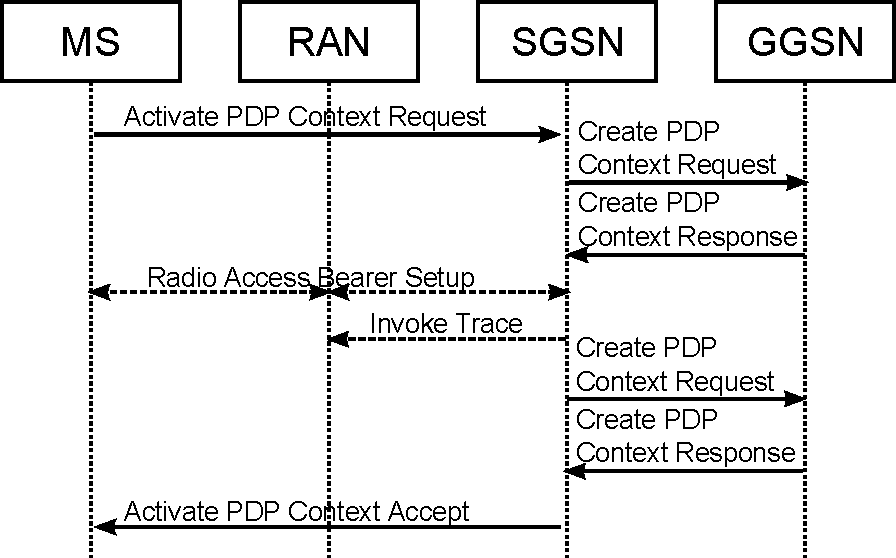
\includegraphics[width=0.8\columnwidth]{images/CONEXT2012/pdp-context-activation.pdf}
\caption{PDP Context Activation Procedure in a UMTS network.}
\label{fig:pdpcontextactivation}
\end{figure}

Figure \ref{fig:pdpcontextactivation} shows the \textit{PDP Context Activation Procedure} as defined in \cite{3gpp23060}. Some additional \ac{CAMEL} procedures may be involved in the creation but are not of interest in the context of this paper as they are not required. Tunneling messages are usually triggered by other procedures on different interfaces. In the case depicted here, the procedure is initiated by the mobile device through a \ac{RANAP} protocol \textit{Activate PDP Context Request} typically sent when establishing a mobile data connection.

Generally speaking, any Create Request is part of a \textit{GPRS PDP Context Activation} procedure, which can happen under several circumstances, the aforementioned one being the typical, but also during each \textit{Secondary PDP context Activation} procedure for every tunnel beyond the first. When a \ac{GGSN} receives this request from an \ac{SGSN}, it attempts to complete the Context creation. Depending on the outcome, a response is sent back, indicating the success or failure of the operation. Typical failure codes observed in our measurements were either due to incorrect information supplied by the device (``user authentication failed''), due to malformed messages (e.g. ``invalid message format''), or indicated problems or temporary overload in the network (``no resources available'' and ``system failure'').




%%%%%%%%%%%%%%%%%%%%%%%%%%%%%%%%%%%%%%%%%%%%%%%%%%%%%%%%%%%%%%%%%%%%%%%%%%%%%%%%
\subsubsection{Update Context Messages}

The possible causes for an \textit{Update Context Request} are as following.

\begin{itemize}
	\item The mobile devices moves between \acp{SGSN}, causing a \textit{GPRS inter-SGSN Routing Area Update} procedure.
	\item Parameters belonging to the context such as the assigned \ac{QoS} are altered using the the \textit{PDP Context Modification}.
	\item As part of \textit{Context redistribution and load balancing} procedures.
	\item The \ac{MS} switches between \ac{UMTS} and \ac{GPRS} access technologies, causing a \textit{Inter-system intra- \\SGSN Update} procedure. Note that the same tunnel can be used regardless of the radio technology.
	\item As part of a direct \ac{RNC} to \ac{GGSN} GTP-U tunnel activation procedure, thereby circumventing the \ac{SGSN}. Or, finally, 
	\item To activate secondary PDP contexts using the \textit{Secondary PDP Context Activation} as previously described. 
\end{itemize}

By observing Update Context message one could, for example, capture most forms of mobility happening in the network, and get a good picture of correlations between mobility and tunneling characteristics. Additionally, tunnels using \ac{UMTS} and \ac{GPRS} radio technology can be distinguished, which should in theory lead to wholly different pictures, as nowadays GSM/GPRS is either used in older models or feature phones, or in mobile scenarios in rural areas where the larger GSM cells are more prevalent. Both could indicate that the data session will be rather short  due to either clumsy devices or the low throughput rates of \ac{GPRS}.

%%%%%%%%%%%%%%%%%%%%%%%%%%%%%%%%%%%%%%%%%%%%%%%%%%%%%%%%%%%%%%%%%%%%%%%%%%%%%%%%
\subsubsection{Delete Context Messages}

The third type of Tunnel Management messages are the \textit{Delete Context Request} and \textit{Response}, indicating the immediate release of the Context involved. They are part of 

\begin{itemize}
	\item The \textit{GPRS Detach} procedure from the \ac{SGSN} to the \ac{GGSN}, when a device completely deactivates its data services.
	\item The \textit{GPRS PDP Context Deactivation} procedure from the \ac{SGSN} to the \ac{GGSN}, if only one specific tunnel is to be removed.
	\item The \textit{part of PDP Context Deactivation Initiated by GGSN} procedure signaled to the \ac{SGSN}.
\end{itemize}



%can also delete a set of contexts assigned to a single MS



%%%%%%%%%%%%%%%%%%%%%%%%%%%%%%%%%%%%%%%%%%%%%%%%%%%%%%%%%%%%%%%%%%%%%%%%%%%%%%%%
\subsubsection{Mobility and Radio-related State Machines}

As indicated before, most nodes in a cellular mobile network keep all sorts of states characterizing the data connection. For the tunnel management aspects, two state machines are of special note.

\begin{figure}
	\centering
	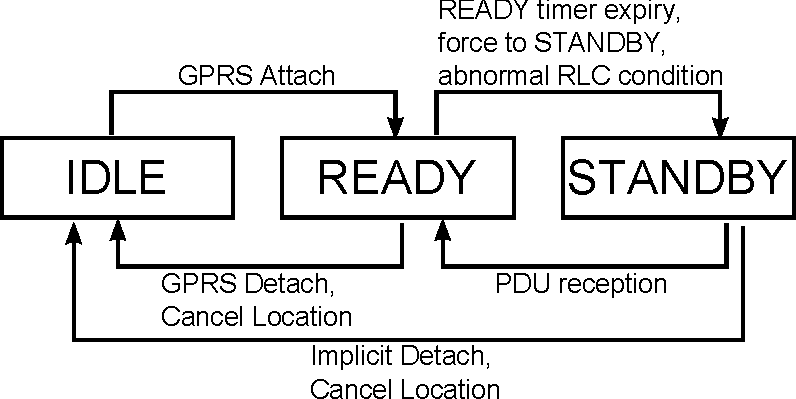
\includegraphics[width=0.7\columnwidth]{images/CONEXT2012/mm-state-model.pdf}
	\caption{SGSN Mobility Management State Model.}
	\label{fig:mmstatemodel}
\end{figure}

First, consider the Mobility Management state machine depicted in Figure \ref{fig:mmstatemodel}, defined in \cite{3gpp23060}, and held in both the \ac{SGSN} as well as the mobile device. It describes the general state of the data connection, and switches states based either on an idle timer, or when new packets arrive for the mobile device. Therefore, it also controls tunnel management, as the involved GPRS Detach and Attach procedures involve deleting and creating contexts. We identify user traffic dynamics as one vector to influence core network signaling, similar to the observations in \cite{lee2007detection}.

\begin{figure}
	\centering
	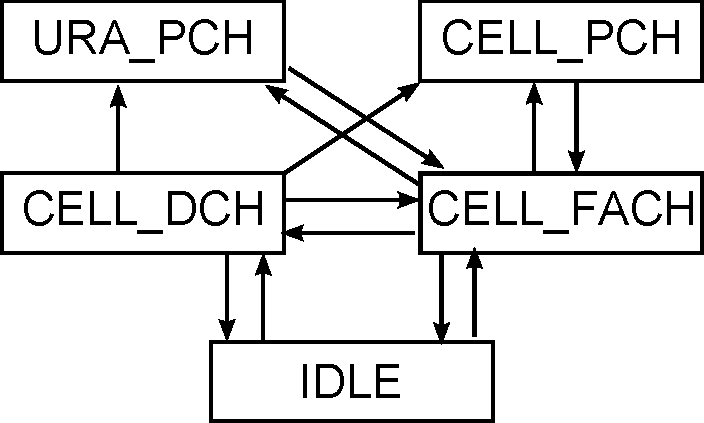
\includegraphics[width=0.6\columnwidth]{images/CONEXT2012/rrc-state-model.pdf}
	\caption{Radio Resource Control State Model.}
	\label{fig:rrcstatemodel-CONEXT}
\end{figure}

The \ac{RRC} state machine shown in Figure \ref{fig:rrcstatemodel-CONEXT} governs the usage of radio channels, i.e. spectral and temporal usage of the wireless interface. State changes happen depending on the inter-arrival time of user packets. In this case, if the state machine transitions to the IDLE state, the \ac{RAB} on the path between mobile device and \ac{SGSN} is not needed anymore and will be deleted, in most cases destroying the SGSN and GGSN PDP Context as well.




%%%%%%%%%%%%%%%%%%%%%%%%%%%%%%%%%%%%%%%%%%%%%%%%%%%%%%%%%%%%%%%%%%%%%%%%%%%%%%%%
\subsection{Discussion of GTP Signaling}

Looking at the Create, Update and Delete PDP Context Request and Reply message pairs we can already deduce a certain amount of information. Measuring the time delta between corresponding Create and Delete events obviously gives the total duration a tunnel was established. Given the amount of user-plane IP traffic transferred, when the tunnel durations are short, we can expect the number of tunnel creation and deletion events to go up instead, resulting in a higher volume of signaling messages and an increase in processing for these messages. Conversely, longer tunnel durations cause an increased overall memory footprint in the involved nodes to store the \ac{PDP} Contexts. Large numbers of update messages, especially combined with frequent \ac{RAT} switches, are usually an indicator for highly mobile devices switching their routing area. This mobility behavior could be investigated by evaluating the update messages.

As discussed, most of the actions in the network as well as in the mobile devices are reflected in the presented tunnel management messaging. Therefore, taking a look at the dynamics of this control aspect in real networks gives valuable insights on the influence of many of the networks' aspects.



%We describe some of the GPRS state models as they have an impact on how long PDP Contexts are held.
%Mobility Management State Transitions
%As per 23.060 GPRS, section 6.1.1.4
%One factor of influencing PDP context creation and deletion is the current mobility management state, held in the SGSN and the mobile device.
%PDP Context gets deleted when the state machine transitions to the IDLE state.
%RRC State Transitions
%When moving the UE to te IDLE state the radio resource bearer on the UE<->SGSN path gets released. This is another possible cause for a PDP context deactivation.

%Correlation to stories about carrier complaints over (radio) ``signalling storms''  and 3gpp R8 Fast Dormancy \cite{3gpp25331} and \cite{gsma2011fdbestpract}


%creates can overwrite existing contexts
%Create Context Response
%Describe the response message types
%GGSN to SGSN
%cause IE; either success or failure reason

%Possible context response types and which request types they answer:
%\begin{itemize}
%\item 192: "non-existent" UPDATE \& DELETE ONLY
%\item 193: "invalid message format" UPDATE \& DELETE ONLY
%\item 199: "no resources available" CREATE ONLY anywhere in the network to allocate context
%\item 200: "service not supported" UPDATE ONLY
%\item 201: "mandatory IE incorrect"
%\item 202: "mandatory IE missing"
%\item 204: "system failure" CREATE \& UPDATE ONLY
%\item 209: "user authentication failed" CREATE ONLY rejected for various reasons
%\end{itemize}



%create context is part of PDP context activation procedure (probably requested by phone to SGSN, negotiated from SGSN to GGSN)
%discuss when this happening; only at phone switch on? mobility? ... 
%request configuration through information elements IE, includes APN (set by phone or SGSN)
%secondary PDP context activation procedure for every tunnel beyond the first (indexed by NSAPI (starting with value 5); packet distinction/filtering by TFT at GGSN
%  secondary contains fewer IEs (selection mode, IMSI, MSISDN, address, APN, APN restriction not included)
%  --> How many contexts do phones hold? --> distribution! differentiation per TAC?




%307 Bytes:
%Total maximum signaling traffic with this calculation: 117.15GB
%Ratio: 0.10\%
%52 Bytes:
%Total maximum signaling traffic with this calculation: 19.84GB
%Ratio: 0.02\%
%Total traffic: 122758578593993



%GTP Header: 12 Byte
%IE header and footer: 2 Byte
%Maximum minimum data size including all \acp{IE}: 221 Byte + 12 Byte Header + 2*37 Extension Header = 307 Byte
%Minium size of mesage with just mandatory \acp{IE}: 12 + 30 + 2*5 = 52 Byte

% Berechnungsgrundlage für die IEs
%\begin{table*}
%\centering
%\caption{Information Elements in a Create PDP Context Request (as peer TS 29.060, Section 7.3.1)}
%\label{tab:createrequestelements}
%\begin{tabular}{|p{4cm}|p{2cm}|p{2cm}|p{4cm}|p{2cm}|p{2cm}|} \hline
%\textbf{Information Element} & \textbf{Presence Requirement} & \textbf{Typical Size} & \textbf{Information Element} & \textbf{Presence Requirement} & \textbf{Typical Size} \\ \hline
%IMSI & Conditional & 9 & TFT & Conditional & min. 4\\ \hline
%Routing Area Identity & Optional & 7 & Trigger Id & Optional & min. 4 \\ \hline
%Recovery & Optional & 2 & OMC Identity & Optional & min. 4 \\ \hline
%Selection mode	& Conditional & 2 & Common Flags & Optional & 4\\ \hline
%Tunnel Endpoint Identifier Data I & Mandatory & 5 & APN Restriction & Optional & 4\\ \hline
%Tunnel Endpoint Identifier Control Plane & Conditional & 5 & RAT Type & Optional & 4\\ \hline
%NSAPI & Mandatory & 2 & User Location Information & Optional & 11\\ \hline
%Linked NSAPI & Conditional & 2 & MS Time Zone & Optional & 5\\ \hline
%Charging Characteristics & Conditional & 3 & IMEI(SV) & Conditional & 11\\ \hline
%Trace Reference & Optional & 3 & CAMEL Charging Information Container & Optional & min. 4\\ \hline
%Trace Type & Optional & 3 & Additional Trace Info & Optional & 12\\ \hline
%End User Address & Conditional & 9 (for IPv4) & Correlation-ID & Optional & 4\\ \hline
%Access Point Name & Conditional & 3 + Name & Evolved Allocation Retention Priority I & Optional & 4\\ \hline
%Protocol Configuration Options & Optional & min. 3 & Extended Common Flags & Optional & min. 4\\ \hline
%SGSN Address for signaling & Mandatory  & 9 (for IPv4) & User CSG Information & Optional & 11 \\ \hline
%SGSN Address for user traffic & Mandatory & 9 (for IPv4) & APN-ABMR & Optional  & 11 \\ \hline
%MSISDN & Conditional & 3 + MSISDN & Max MBR/APN-ABMR & Optional & min. 11 \\ \hline
%QoS Profile & Mandatory & min. 5 & Private Extension & Optional & min 6\\ \hline
%Signaling Priority Indication & Optional & min. 4 & & & \\ \hline
%\end{tabular}
%\end{table*}


%\begin{itemize}
%\item TS 29.060 GTP protocol description (SGSN-GGSN)
%\item TS 23.060 GPRS control procedure description (incl pdp context activation proc)
%\end{itemize}

% \subsubsection{Information Element Concept}
% Discuss the concept
% list all involved IEs their sizes and thus the imposed overhead
% "The IMSI IE together with the NSAPI IE uniquely identifies the PDP context to be created"



%%%%%%%%%%%%%%%%%%%%%%%%%%%%%%%%%%%%%%%%%%%%%%%%%%%%%%%%%%%%%%%%%%%%%%%%%%%%%%%%
\section{Network and Monitoring Setup}
\label{sec:darwin-CONEXT}


%\begin{figure*}%[tbp]
%\centering
%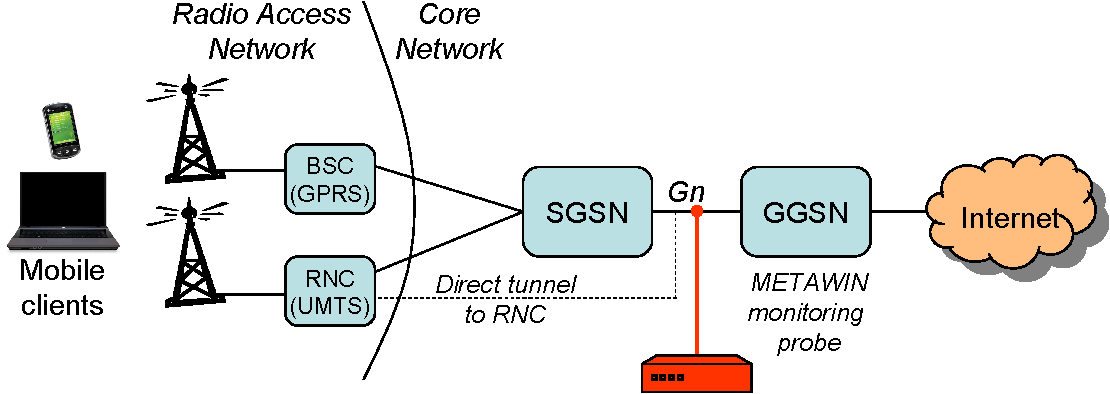
\includegraphics[width=0.98\textwidth]{figures/network_setup_gtp_tun-crop.pdf}
%\caption{Measurement setup.}
%\label{fig:net_setup}
%\end{figure*}

For our analysis, we use the \ac{METAWIN} monitoring system developed in a previous research project
and deployed in the network of an Austrian mobile operator.  More in-depth information about \ac{METAWIN} is available in \cite{ricciato_2011}.
The location of the measurement probe within the core network is highlighted in Figure~\ref{fig:umtsnetwork}. 

As said before, the \ac{GGSN} acts as the IP-layer gateway for the user traffic. It is in charge of setting up,
maintaining, and tearing down a logical connection to each active \ac{MS}. This logical connection, the \ac{PDP} context,
is conceptually similar to a dial-up connection. During set up, an
IP address is dynamically assigned to the \ac{MS}.
%The \acp{SGSN} and \acp{GGSN} in the core network are interconnected by a wide-area IP network that
%will be referred to as the ``G$_n$ network'' following the terminology of \ac{3GPP} specifications
%(``Gn interface'').
In the network under study, a so-called \textit{direct tunnel} setup might be used for \acp{MS} connected
via \ac{UMTS}/\ac{HSPA}. Such a setup consists of a direct link between \acp{GGSN} and the
\acp{RNC} %(indicated by the upper dashed line in Fig.~\ref{fig:umtsnetwork}), % Dashing is indiscernible in the figure.
which is used for
transporting user-plane data traffic only. Since signaling procedures such
as mobility management are carried out by the \acp{SGSN}, a \ac{GGSN} always has to send signaling packets
via the path involving the \acp{SGSN}. Monitoring the Gn interface thus gives us access to both wide-area mobility signaling (not analyzed in this paper) % routing area updates
and signaling related to user-plane IP traffic (which we want to scrutinize).
For more information on the \ac{3G} network structure, please refer to~\cite{bannister_convergence_2004}.

The METAWIN monitoring system extracts and correlates information from the lower
layers of the \ac{3GPP} protocol stack, and specifically the \ac{GTP} protocol
on the Gn interface \cite{etsi_3gpp_2008}. This includes the \acf{RAT} identifier as well as the terminal types of the mobile clients. The
latter is determinable by the \acf{TAC} part of the \acf{IMEI} (cf. \cite{3gpp23003}) and will be discussed later in detail.

To meet privacy requirements, the METAWIN system anonymizes captured data on the fly at multiple
layers: the application-level payload is removed and all user identifiers (e.g. \ac{IMSI}) are
hashed with a one-way function before recording. That is, single
\acp{MS} in our dataset may be differentiated by means of an anonymized \ac{MS-ID}, but not traced back to the actual customer.
The packet capturing hardware deployed within the METAWIN monitoring system is synchronized
using \ac{GPS}. Accordingly, the packet timestamps
have an accuracy of $\pm100$ ns or better~\cite[p.97-98]{donnelly_high_2002}.



%%%%%%%%%%%%%%%%%%%%%%%%%%%%%%%%%%%%%%%%%%%%%%%%%%%%%%%%%%%%%%%%%%%%%%%%%%%%%%%%
\section{Evaluation}
\label{sec:evaluations-CONEXT}

In this section we attempt to shed some light on the overall control plane dynamics in a mobile core network. We evaluate a dataset recorded in a live 3G network for PDP Context durations, and attempt to show the possible impact of certain device categories on the total tunnel durations. As discussed before, this can serve as a proxy metric for the signaling load on the system. 


%%%%%%%%%%%%%%%%%%%%%%%%%%%%%%%%%%%%%%%%%%%%%%%%%%%%%%%%%%%%%%%%%%%%%%%%%%%%%%%%
\subsection{Dataset Description}
Our dataset, kindly provided by an Austrian mobile operator and recorded using the \ac{METAWIN} monitoring system, was taken in the third week of April 2011. It consists of seven days of aggregated flow-level data for the user traffic and a summary entry for every \ac{GTP} Tunnel Management transaction, the latter representing the data base for this paper. It was tapped at one of the \acp{GGSN} of the operator, and contains about half of the total traffic volume handled by the operator in this period. The \ac{GTP} data contain the response codes for each transactions. With these codes, failed interactions can be sorted out and treated separately.

We fed the records into a SQL database, and conducted further evaluations through scripted queries on the database. Any privacy-relevant data, e.g. the \ac{IMEI}, \ac{MS-ID} and any IP address involved, is only visible as hashes and can only be processed in anonymized form. Individual device types can be identified in form of the unhashed \ac{TAC} on every entry. Since the hashing of the \ac{IMEI} is consistent, user traffic flows and the \ac{GTP} data can be cross-correlated despite anonymization, giving the opportunity for further research.

 

%%%%%%%%%%%%%%%%%%%%%%%%%%%%%%%%%%%%%%%%%%%%%%%%%%%%%%%%%%%%%%%%%%%%%%%%%%%%%%%%
\subsection{Factors Influencing Tunnel Durations}

With such a dataset available and with the intent to evaluate core network signaling by looking at tunnel durations, let's first discuss some of the factors that influence this duration.

One factor are the mobile devices themselves. The device decides when it should establish a mobile data connection, how long the connection is held, or which mobile technology takes preference. Devices can be further differentiated by their operating system and their firmware (sometimes called \textit{baseband}) which usually takes care of much of layers 1 and 2.

Some specific tunnel durations could stem from the TCP/IP stack implementations in the operating systems of the devices. TCP timeouts might be configured to different default values in different releases of OSs. Also, mobile network firewalls have been found to interfere with transport and application-layer timeout and keep-alive or heartbeat mechanisms on mobile devices \cite{sigcomm11middleboxes}.

Of course, the applications that run on top of the OS and generate the actual user-traffic patterns play a role as well. An example for how applications can influence network signaling is the casual game ``Angry Birds'' mentioned before. Since the application ecosystem for smartphones is extremely rich (and grows still), we cannot pinpoint individual ones from our aggregate dataset.

An additional factor in the picture is the user and his or her behavioral patterns. They express themselves both in the traffic dynamics and in the mobility pattern, but they are rather difficult to distinguish in such a dataset given the large amount of data and the difficulty of correctly correlating tunnel management messages. We leave this as a potential future work.

We also expect the mobile network and its protocol implementations to express themselves in the measurements. For example, the \ac{RRC} idle timer is typically in the range of 10 to 30 minutes, which could mean there will be a large number of tunnels with a duration in this range. Such choices are usually made either by the mobile network operator or the device manufacturer and can vary from one implementation to another. It is therefore quite difficult to give any hard numbers in advance, and one has to correlate such aspects with certain events in the results.

Based on these factors, it was decided to make a first categorization according to the device type, be it either a smartphone, a regular or feature phone, or one of the many 3G dongles or mobile routers. Second, we also differentiate based on the device operating system, if known. Both differentiating aspects should prove valuable for example in deciding if currently some phone types put more signaling load on the network and to direct measures to improve this situation. Pitfalls in this differentiation are described in the next sections.



%%%%%%%%%%%%%%%%%%%%%%%%%%%%%%%%%%%%%%%%%%%%%%%%%%%%%%%%%%%%%%%%%%%%%%%%%%%%%%%%
\subsection{Difficulties of Device-based Evaluations}

In our dataset, the \ac{TAC} field is provided in clear\-text, whereas the \ac{IMEI} is only available in hashed form to preserve the privacy of device owners. The \ac{TAC} is contained in the first eight decimal digits of the \ac{IMEI}, uniquely identifying each device type \cite{3gpp23003}. The rest of the \ac{IMEI} constitutes the serial number of the involved devices.

\acp{TAC} are managed by the GSM Association which in turn assigns local organizations, distinguished by the first two digits of the \ac{TAC} as Reporting Body Identifier, to allocate \acp{TAC} to manufacturers. For reasons beyond us, this allocation information is not freely available. Commercial databases exist, but this is neither affordable for research institutions, nor is it conducive to our goal of providing information to the public. While there are some websites that allow one to query for specific \acp{TAC} for non-commercial purposes, only very few efforts to collect \ac{TAC} information into a database are publicly available. We based our data-mining efforts on a set from \cite{tacdb}, with some additional devices with known \ac{TAC} collected from various sites, friends, and colleagues. Since the unit identification part of the \ac{IMEI} is just six decimal digits long, popular devices will even be assigned more than one TAC, making the acquisition of all relevant \acp{TAC} even more complicated.



%%%%%%%%%%%%%%%%%%%%%%%%%%%%%%%%%%%%%%%%%%%%%%%%%%%%%%%%%%%%%%%%%%%%%%%%%%%%%%%%
\subsection{Device Classification}

For our investigation, we went through large portions of the \acp{TAC} present in our dataset, and identified and categorized the most important entries. In this case, importance means various metrics like the traffic volume, the number of flows, and the number of \ac{GTP} signaling messages for each \ac{TAC}. 

After having available the device names for most \acp{TAC}, we were able to add meta-information to the entries in form of the following categories:

\begin{itemize}
\item The device type. We distinguished between smartphones, regular mobile phones and feature phones, and 3G USB dongles or 3G/WiFi routers.

\item The operating system of the device (if known), such as Android, iOS, Series 40, BlackBerry OS etc. This is especially interesting to identify potential differences in the core network signaling patterns of devices. Note however that we cannot link USB dongles and OS types from the \ac{TAC}.

\end{itemize}







%%%%%%%%%%%%%%%%%%%%%%%%%%%%%%%%%%%%%%%%%%%%%%%%%%%%%%%%%%%%%%%%%%%%%%%%%%%%%%%%
\subsection{\acs{TAC} Statistics and Evaluation Validity}

\begin{table}
\centering
\caption{Relative \acs{TAC} Statistics.}
\label{tab:tacstats-CONEXT}
\begin{tabular}{|p{4cm}|p{3cm}|} \hline
& \textbf{Portion of devices with entry in TAC DB}\\ \hline
\# of Flows & 99.72\% \\ \hline
Ratio of Traffic & 99.97\%\\ \hline
\# of Tunnels & 87.57\% \\ \hline
\# of GTP Signaling Msgs & 90.95\% \\ \hline
\# of Distinct \acp{MS-ID} & 80.93\%\\ \hline
\end{tabular}
\end{table}


It is important to know whether our \ac{TAC} mappings provide sufficient useful data to allow for the envisioned device discriminating statistics. Therefore, Table~\ref{tab:tacstats-CONEXT} provides some statistics on our knowledge of devices in the dataset. About 80 percent of all  distinct devices active could be identified. Looking at the total number of \ac{GTP} signaling messages, we see that we can determine the device name of over 90 percent.
The flow data shows an even clearer picture, as we can identify almost all of the devices involved.


After applying the categorization to the \acp{TAC} we evaluate the device composition in the network. The two largest portions of devices are smartphones  and 3G dongles, while classic cell phones do not seem to play a major role anymore. 
%We see about twice as many Android as iOS devices, possibly attributed either to the contractual situation of the operator or the wider price range of Android devices.

%Regular phones have negligible user traffic despite still making up one tenth of the device fraction. 

Initially, one planned endeavor was to investigate possible peculiarities of business phone behavior, especially of those easily identifiable Blackberry OS phones, but the number of distinct Blackberry devices in the dataset is too low to draw conclusions of any significance.

One observation across all device types is that about 18 percent of all mobile devices have activated their mobile data service and have signaling traffic, but do not cause any use plane traffic.

The difference between 3G dongles and smartphones is also noteworthy. While the former cause large amounts of user plane traffic (compared to the device numbers), they are responsible for but a low number of core network signaling events and tunnels. This picture is reversed for smartphones.





%%%%%%%%%%%%%%%%%%%%%%%%%%%%%%%%%%%%%%%%%%%%%%%%%%%%%%%%%%%%%%%%%%%%%%%%%%%%%%%%
\subsection{PDP Context Durations}

Our measure of choice are the PDP Context Durations as they carry lots of meaning in being directly related to the signaling amount in the network. Therefore, we now direct our attention at the tunnel durations in the individual device and OS categories as identified via \ac{TAC} values.


\subsubsection{Tunnel Durations by Category}

\begin{figure}
	\centering
	\includegraphics[width=\columnwidth]{images/CONEXT2012/tunnel-dur-class-cdf-mod.pdf}
	\caption{Tunnel duration distribution, separated for 3G dongles, smartphones and regular phones with medians at 115s (Total), 31s (Regular), 82s (Smartphone), and 1207s (3G Dongle)}
	\label{fig:cdf-duration-device-class-CONEXT}
\end{figure}

Figure~\ref{fig:cdf-duration-device-class-CONEXT} shows the empirical cumulative distribution functions for the PDP Context durations in our dataset. We distinguish the total duration distribution as well as the the distributions for smartphones, regular phones, and 3G dongles. It can be observed that tunnel durations range between  seconds and more than one week\footnote{Although our dataset is one week long, some tunnels started before the beginning of that week, and ended within it. Since the tunnel start dates were still available from the system, we chose to include the data.}.

The median differs between device types, being much longer for 3G dongles than for mobile phones. This can probably be expected, as typical dongle sessions might involve working at a laptop for periods longer than a few seconds or minutes. Also for the dongles, we observe less extremely long tunnels with durations above several hours. Again, we could hypothetically relate this to a usual laptop working environment, where the device is used for a few hours but then shut down. With this, the PDP Context is deleted as well. Interestingly, the median duration of regular phones is higher than that of smartphones. This may indicate that  smartphones regularly (and perhaps automatically) cause data traffic and therefore tunnels to occur. We conjecture this to be a first indication of the ``Angry Birds'' effect of automatically transferring small amounts of data, e.g. weather reports, stock exchange data, RSS feeds, or email notifications. We also observe two distinct steps, one at 6.8 seconds for dongles, and one at 30 minutes in the overall and smartphone distributions. While we do not have a plausible explanation for the former, the latter could be explained by a value chosen for the RRC state machine transition to the IDLE state (cf. Figure \ref{fig:rrcstatemodel}).


%%
% Influence of the Device Operating System
%%

\begin{figure}
	\centering
	\includegraphics[width=\columnwidth]{images/CONEXT2012/tunnel-dur-os-cdf-mod.pdf}
	\caption{Tunnel duration cumulative distribution function, separated for Android and iOS devices; Medians at 115s (Total), 15.5s (Symbian), 104s (iOS), and 765s (Android)}
	\label{fig:cdf-duration-os-CONEXT}
\end{figure}

Taking an even closer look at the smartphone device fraction, we can still observe major differences as depicted in the empirical cumulative distribution functions of Figure~\ref{fig:cdf-duration-os-CONEXT}. The tunnel duration distribution of the Symbian device fraction behaves much closer to the regular phones already depicted in Fig.~\ref{fig:cdf-duration-device-class-CONEXT}. A possible explanation could be the user-base being more traditional, or the devices being feature phones whose behavior clearly differs from smartphones.

Again, a number of steps are visible in the distributions. %Steps at multiples of 10 seconds indicate that timer-induced transitions happen. 
Those steps that are only visible in one operating system type point to a source involving the phone rather the network. This especially includes the 30 seconds, 300 seconds, and 600 seconds steps (i.e. accumulations of incidents) for Android, and the 600 seconds step for iOS devices. However, whether this behavior should be attributed to the operating systems themselves cannot be decided by only looking at these distribution. Other factors, e.g. the device's firmware version and user traffic dynamics need also be observed. We leave this point for future work..

A last artifact of note are the larger number of iOS devices with very short tunnel durations. Over 20\% of all tunnels established by these devices are shorter than two seconds. While the actual cause still remains unknown, it could be an interaction between short regular traffic burst and 3GPP Fast Dormancy \cite{gsma2011fdbestpract} which iOS devices are known to implement. Fast Dormancy is a technique to release radio resources more quickly. It is deemed to improve device battery life, radio signaling and radio spectrum efficiency. However, due to the earlier and more frequent transition to the IDLE state, it also could cause an increase in core network tunnel management signaling, which is probably what happened in the iOS case depicted in the CDF.





%%
\subsubsection{Impact of Categories on Total Signaling}
%%

%\vskip -10cm

\begin{figure}
%\vskip -2.5cm
        \centering
        % \begin{subfigure}[b]{0.50\textwidth}
        %         \centering
        %         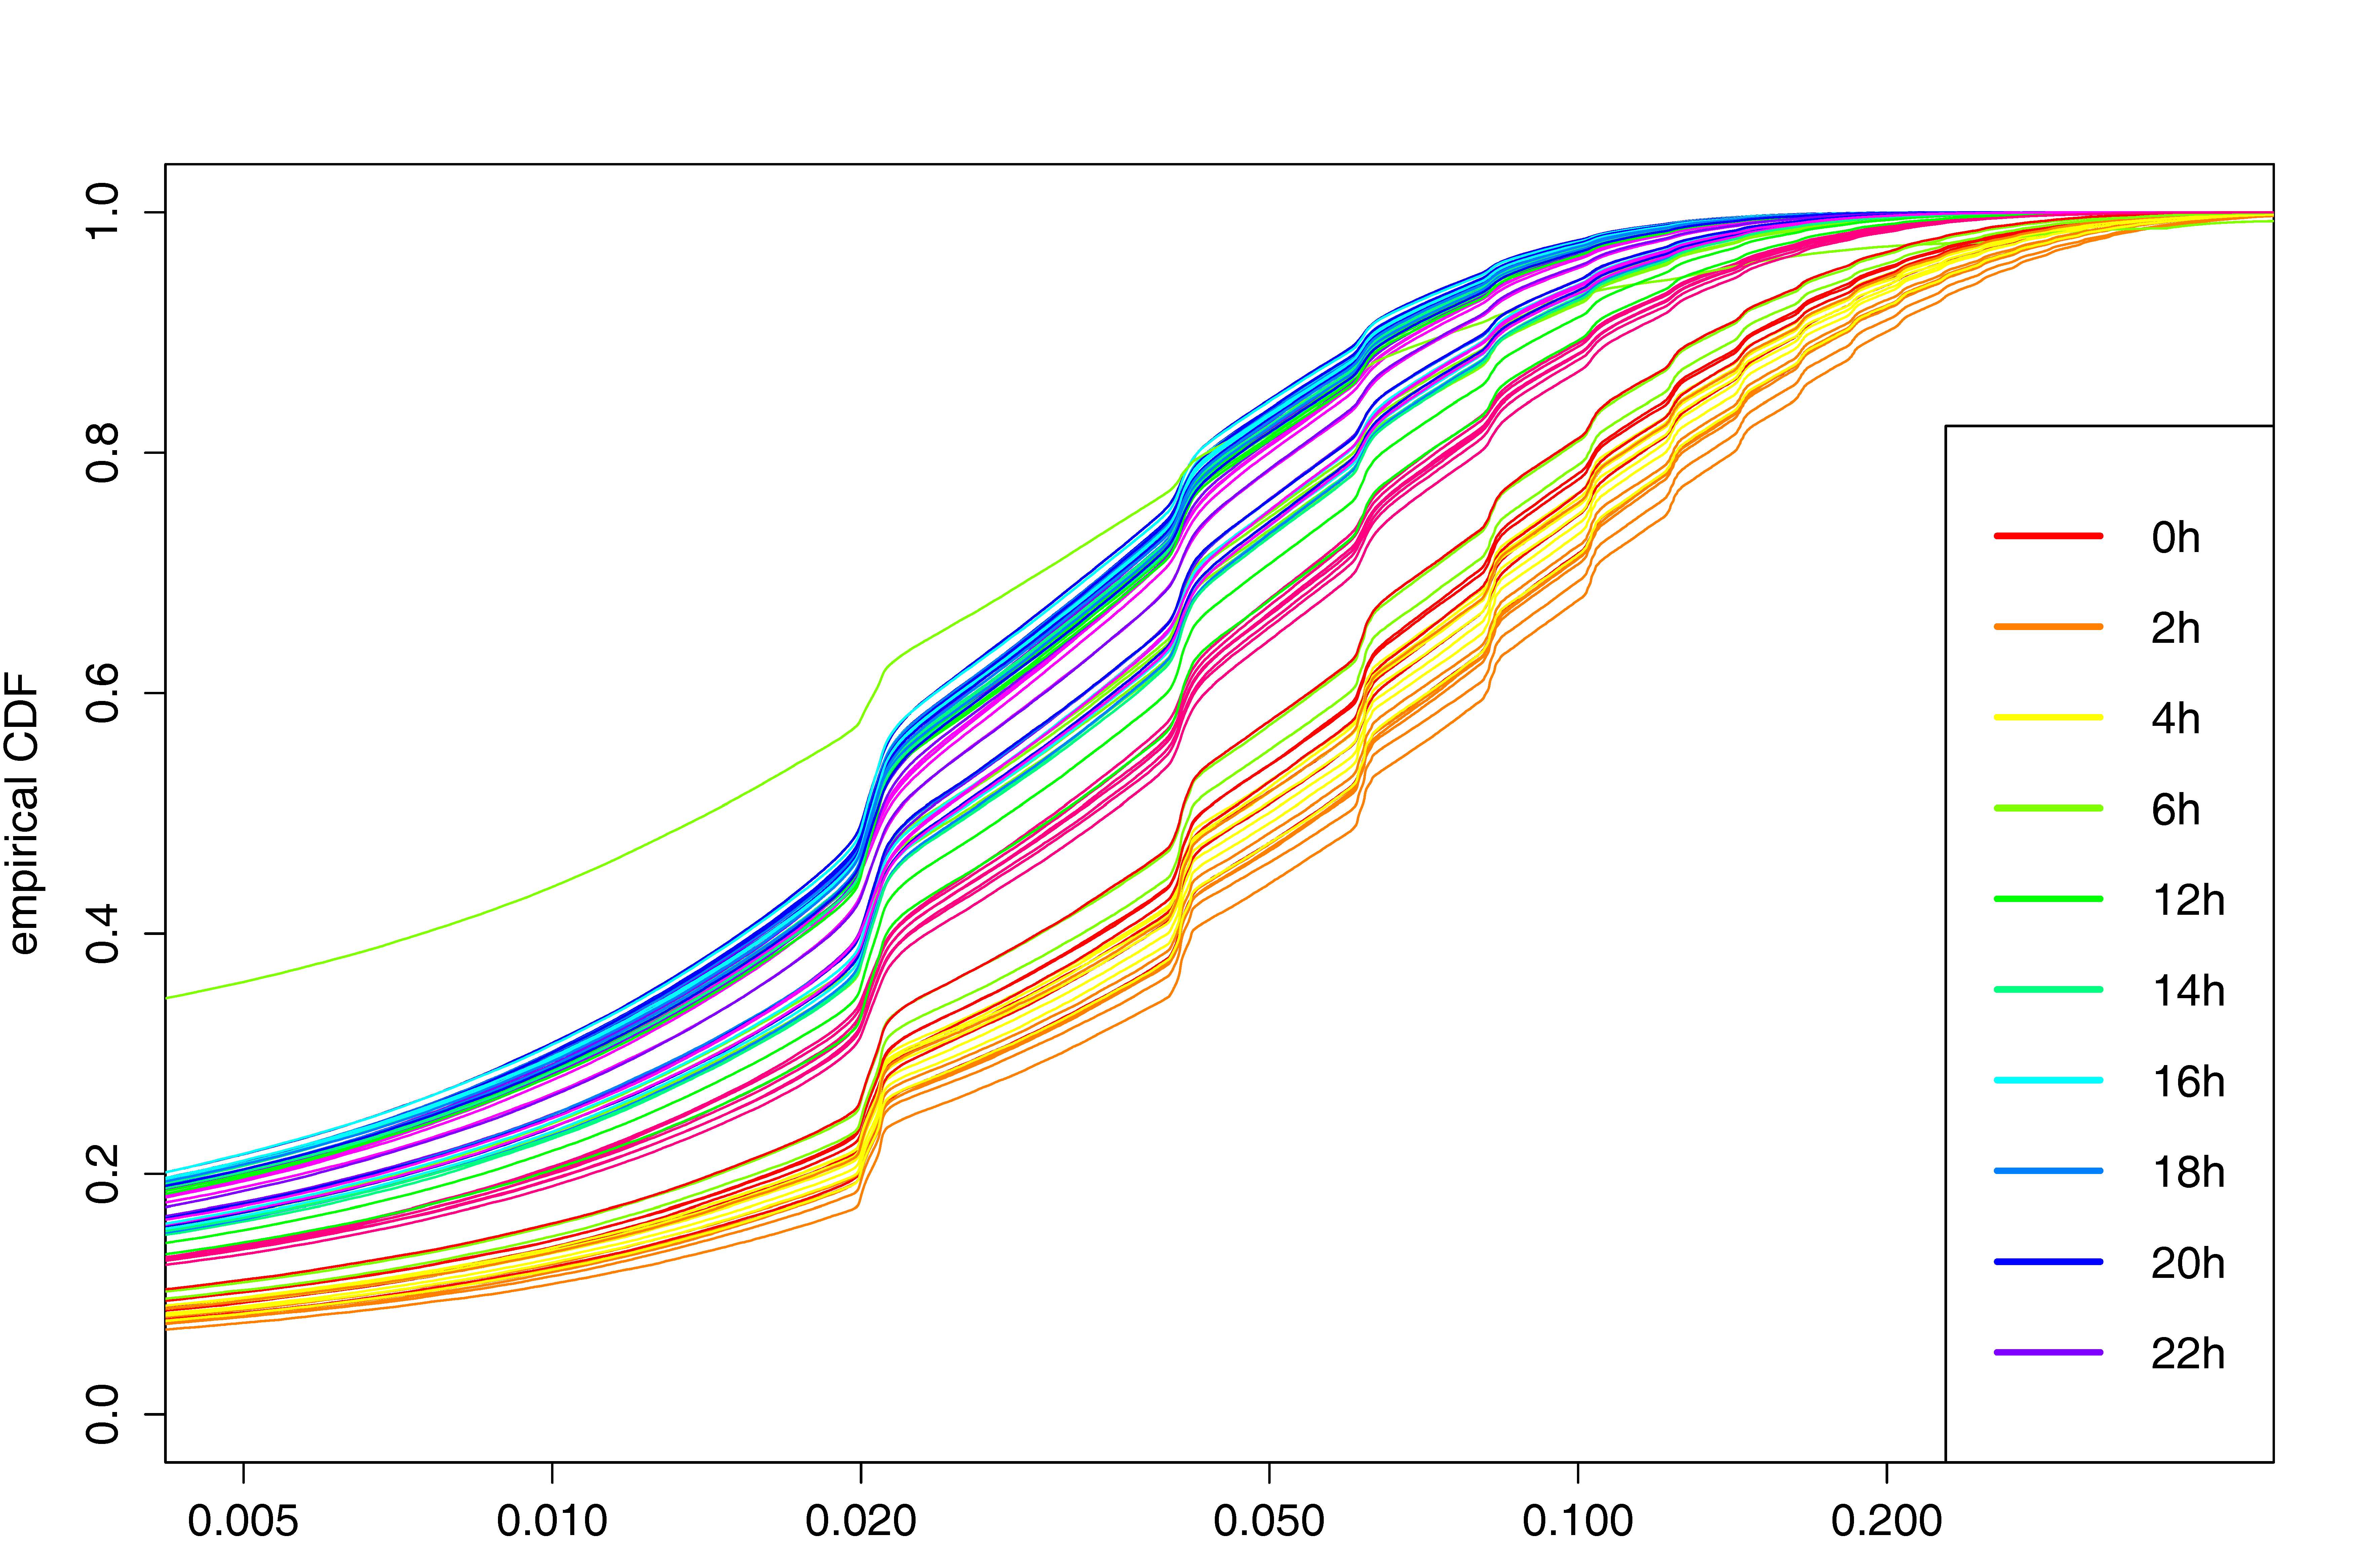
\includegraphics[width=\textwidth]{figures/R-IAT-ecdf-2h-log.png}
        %         \caption{All incoming tunnel requests.}
        %         \label{fig:IAT-ecdf-2h-all}
        % \end{subfigure}%
        %~ %add desired spacing between images, e. g. ~, \quad, \qquad etc.
          %(or a blank line to force the subfigure onto a new line)
        \begin{subfigure}[b]{0.50\textwidth}
                \centering
                \includegraphics[width=\textwidth]{images/CONEXT2012/qq-total-vs-android.pdf}
                \caption{Android duration distribution over the total duration distribution.}
                \label{fig:qq-total-vs-android}
        \end{subfigure}%
        ~
        \begin{subfigure}[b]{0.50\textwidth}
                        \centering
                \includegraphics[width=\textwidth]{images/CONEXT2012/qq-total-vs-ios.pdf}
                \caption{iOS duration distribution over the total duration distribution.}
                \label{fig:qq-total-vs-ios}
        \end{subfigure}

        \begin{subfigure}[b]{0.50\textwidth}
                        \centering
                \includegraphics[width=\textwidth]{images/CONEXT2012/qq-total-vs-dongle.pdf}
                \caption{3G Dongle duration distribution over the total duration distribution.}
                \label{fig:qq-total-vs-dongle}
        \end{subfigure}%
        ~
        \begin{subfigure}[b]{0.50\textwidth}
                        \centering
                \includegraphics[width=\textwidth]{images/CONEXT2012/qq-total-vs-smartphone.pdf}
                \caption{Smartphone duration distribution over the total duration distribution.}
                \label{fig:qq-total-vs-smartphones}
        \end{subfigure}
 \caption{Q-Q Plots of the tunnel duration distributions per operating system, with encircled deciles.}
\label{fig:qq-plots}
\end{figure}

% \begin{figure}
% %\vskip -3cm
% \noindent\makebox[\textwidth]{\subfloat[Android duration distribution over the total duration distribution.]{\label{fig:qq-total-vs-android}\includegraphics[width=\columnwidth]{images/qq-total-vs-android.pdf}}
% \hfil
% \subfloat[iOS duration distribution over the total duration distribution.]{\label{fig:qq-total-vs-ios}\includegraphics[width=\columnwidth]{images/qq-total-vs-ios.pdf}}}
% \noindent\makebox[\textwidth]{\subfloat[3G Dongle duration distribution over the total duration distribution.]{\label{fig:qq-total-vs-dongle}\includegraphics[width=\columnwidth]{images/qq-total-vs-dongle.pdf}}
% \hfil
% \subfloat[Smartphone duration distribution over the total duration distribution.]{\label{fig:qq-total-vs-smartphones}\includegraphics[width=\columnwidth]{images/qq-total-vs-smartphone.pdf}}}
% \caption{Q-Q Plots of the tunnel duration distributions per operating system, with encircled deciles.}
% \label{fig:qq-plots}
% %\vskip -2cm
% \end{figure}


In an attempt to show which of the presented categories have an impact on the total duration (if at all), we present Q-Q plots of the various categorized durations against the total duration in Figure~\ref{fig:qq-plots}. In theory, if both durations follow the same distribution, one expects a straight line through the origin at an angle of 45$^o$. A steeper incline indicates less densely spaced values in the distribution at the y axis. Looking at igures~\ref{fig:qq-total-vs-android} and \ref{fig:qq-total-vs-ios} which compare different operating systems, both similar and dispersing parts can be observed. While tunnel durations on Android  are more similarly distributed for the shorter and longer durations, iOS device tunnel durations are most similar to the overall tunnel duration distribution in the middle range of values.

Combining all types of smartphones together and comparing them to the other major player in any mobile network, the 3G dongles, we observe in Figure \ref{fig:qq-total-vs-smartphones} that both the total and the smartphone durations are almost equally distributed (except for minor variations). On the other hand, 3G dongles follow a very different distribution, see Figure \ref{fig:qq-total-vs-dongle}. Their effect on tunnel management signaling seems to be negligible despite the  large amount of traffic they are causing. Therefore, we conclude that planning and dimensioning of the control plane needs to keep smartphone behaviors more closely in mind than that of other device types.


\begin{figure}
\centering
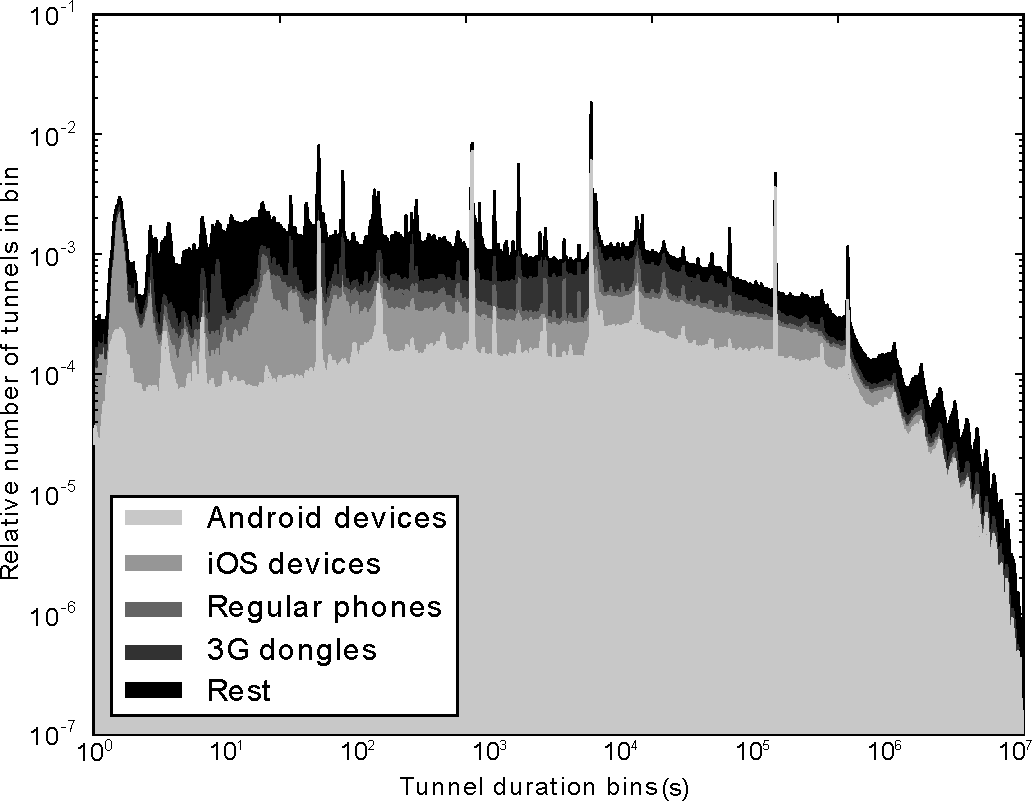
\includegraphics[width=0.75\textwidth]{images/CONEXT2012/stacked-durations-2-fixed.pdf}
\caption{Stacked logscale bin plot of the number of tunnels with duration in this bin; classified by Android, iOS and 3G dongles.}
\label{fig:stacked-durations}
\end{figure}

Figure~\ref{fig:stacked-durations} shows another interesting influence the operating system has on signaling in the mobile core network. This plot shows the relative number of tunnels with a duration in one of 1000 logarithmically scaled bins, stacked by OS category on top of each other. As with the separate distributions, we discover that the durations are not evenly distributed, but rather follow sharp spikes. The largest spike across all categories is the one at a duration of 30 minutes, making up about 1.8\% of all tunnels in the network. Since this spike happens across all device types, we think this makes a rather strong case for being network-induced, and an indication for the aforementioned possible IDLE state transition. On the other hand, the bulk in the short-to-medium ranges of tunnel duration is rather not governed by the two major smartphone operation systems but by other devices in the network, which do not show major spikes in other bins. We can also recognize a long-tail behavior in the distribution of tunnel durations.

%iOS: over 20\% of tunnels shorter than two seconds. 

%\begin{table*}
%\centering
%\caption{Relative \acs{TAC} Statistics.}
%\label{tab:tacstats}
%\begin{tabular}{|p{4cm}|p{2cm}|p{2cm}|p{2cm}|p{2cm}|p{2cm}|} \hline
%& \textbf{\# of Flows} & \textbf{Ratio of Traffic} & \textbf{\# of Tunnels} & \textbf{\# of GTP Signalling Msgs} & \textbf{\# of Distinct \acp{MS-ID}}%\\ \hline
%Total 			& 2234659247 	& 122758578593993	& 16632094 	& 409733865	& 1255293 (from GTPdb) / 1030895 (from flow db) \\ \hline
%Have entry in TAC DB 	& 99.72\% 	& 99.97\%	& 87.57\% 	& 90.95\% 	& 80.93\% \\ \hline
%Classified as smartphone& 20.58\% 	& 12.81\%	& 60.31\% 	& 75.99\% 	& 37.97\% \\ \hline

%as regular phone 	& 0.26\% 	& 0.37\%	& 5.40\% 	& 0.94\% 	& 9.25\% \\ \hline
%as 3G dongle		& 66.55\% 	& 75.12\%	& 12.71\% 	& 9.53\% 	& 25.10\% \\ \hline
%Running on Android	& 10.82\% 	& 6.48\%	& 14.33\% 	& 43.33\% 	& 14.01\% \\ \hline
%iOS			& 7.22\% 	& 4.47\%	& 18.91\% 	& 20.35\% 	& 7.94\% \\ \hline
%S40 / S60 / Symbian	& 1.02\% 	& 1.09\%	& 21.17\% 	& 4.51\% 	& 12.97\% \\ \hline
%Blackberry OS		& 0.07\% 	& 0.10\%	& 2.17\% 	& 2.60\% 	& 1.48\% \\ \hline
%\end{tabular}
%\end{table*}



%%
% Influence of the Radio Access Type
%%
%TODO: radio access type plots, if we have the data
%
%\begin{figure}
%\centering
%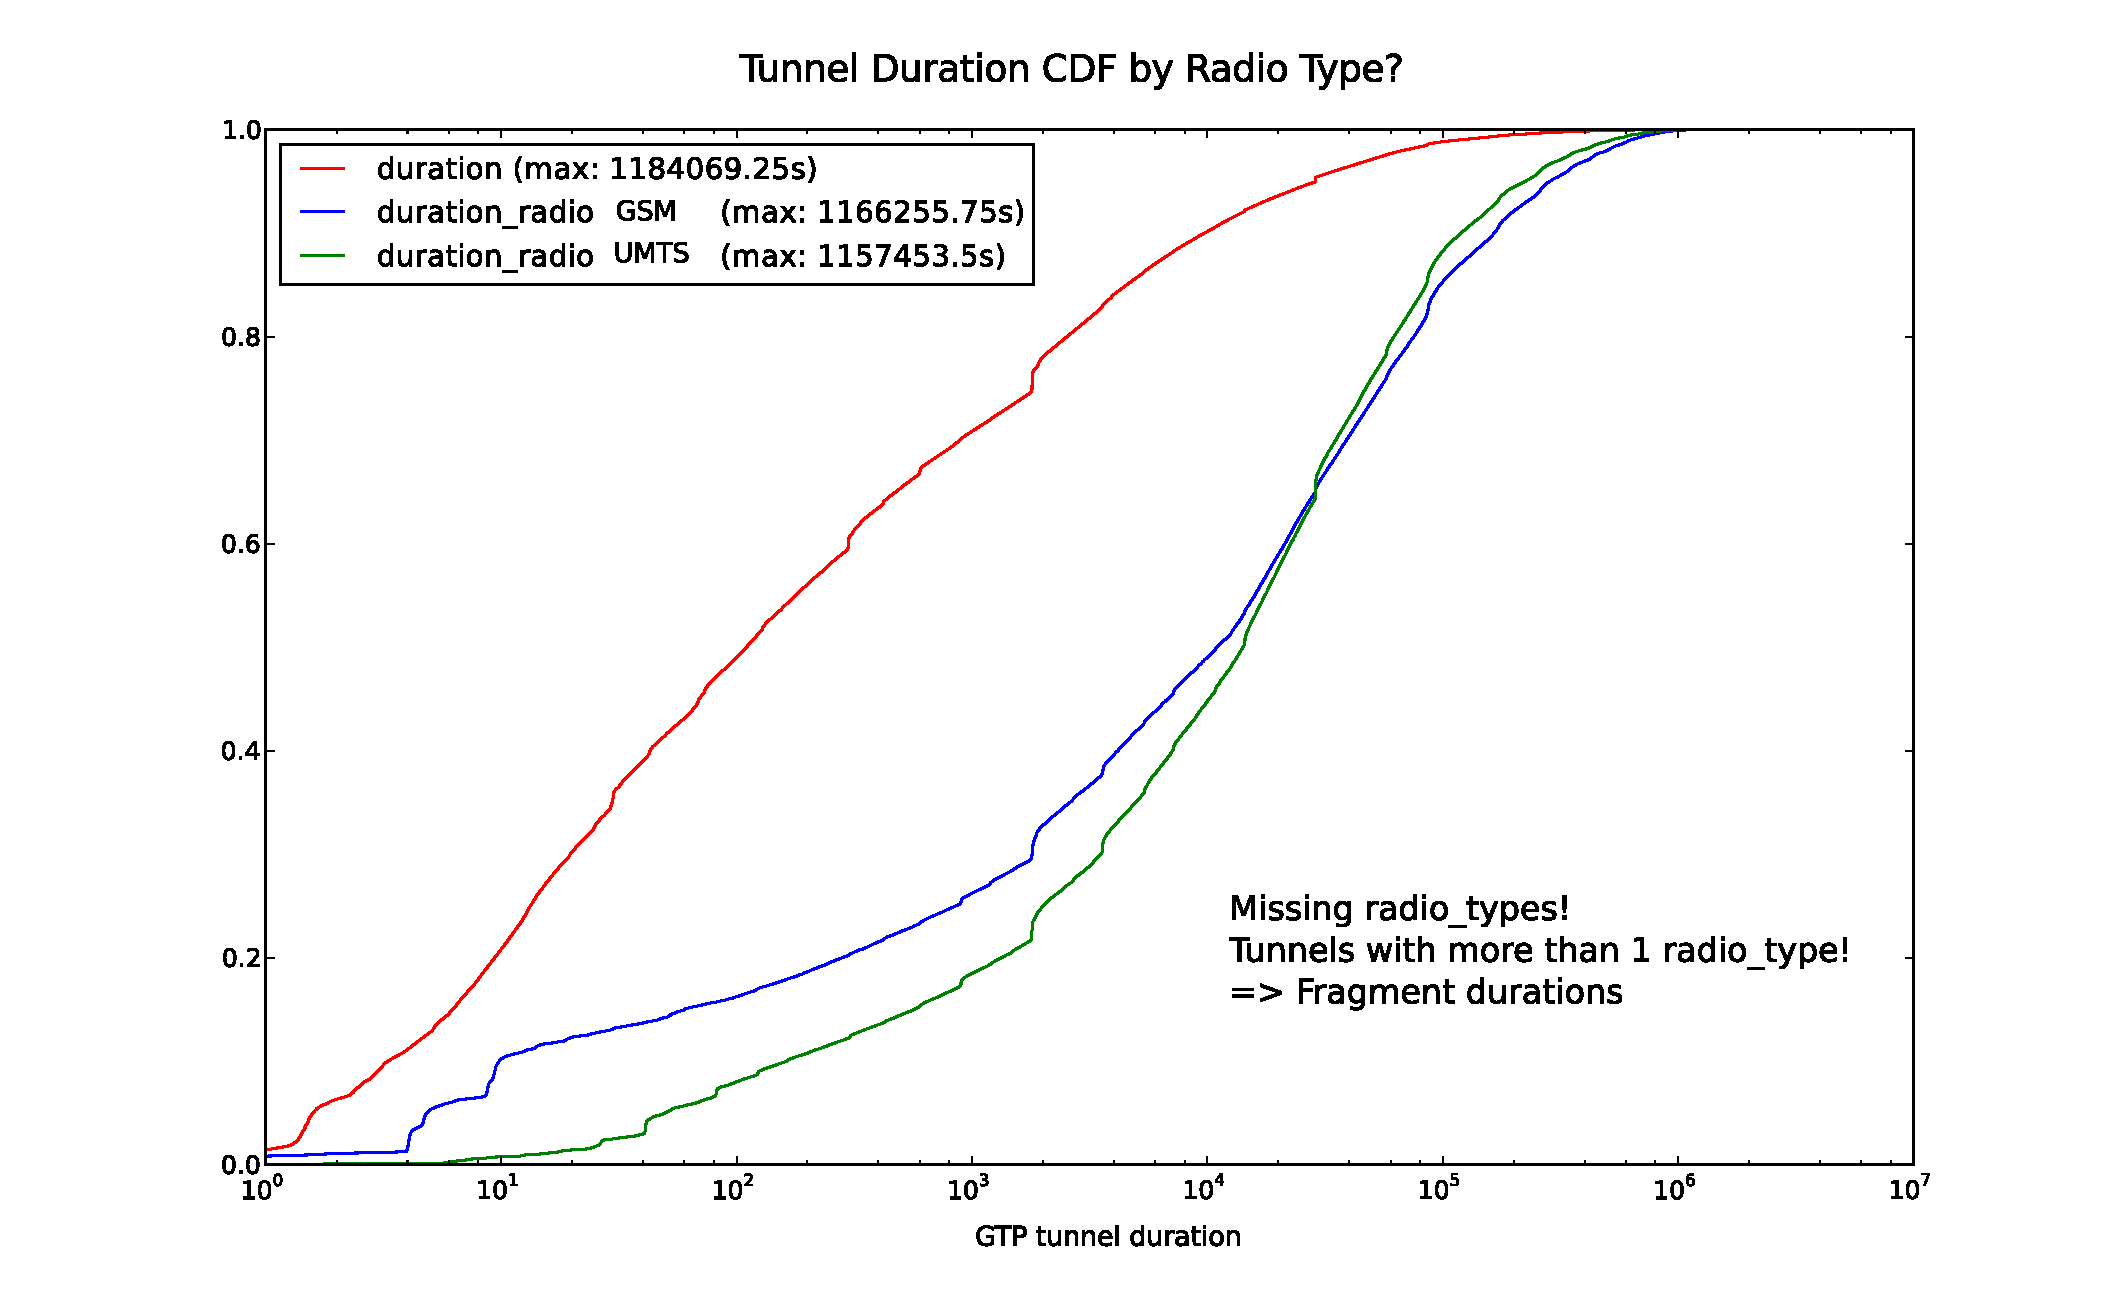
\includegraphics[width=\columnwidth]{figures/tunnel-dur-radio-cdf-mod.pdf}
%\caption{Tunnel duration distribution, separated for UMTS and GPRS radio access [NOTE: only in the last tunnel segment; and majority of radio types %is unknown anyway.}
%\label{fig:cdf-duration-radio}
%\end{figure}

% 10/30m jumps can be seen on android, but not on iOS, why?
%  maybe fast dormancy?

%Corner Cases: 
% - Tunnels active longer than the measurement duration, i.e. either CREATE or DELETE message outside of the one week time span


%We search for factors influencing tunnel durations, and discuss if and how we can observe them in the data set. Thereafter we build up our proposed classification based on these factors.

% User behavior factors, mobility
% Factors from the device: OS, firmware
% Network side factors
% Protocol factors: RRC state change, timeouts

% typical CELL\_PCH to IDLE transition timer 10 to 30 mins
% does/can this influence core sgsn<->ggsn tunnels?
% when is a tunnel deleted?
% data can still flow when in CELL\_PCH, so probably only in IDLE?
% give references to specs!

%On of our goal in our evaluation was to distinguish between certain device types and classes. 

%\begin{table}
%\centering
%\caption{TAC Statistics}
%
%\begin{tabular}{|p{2cm}|p{2cm}|p{2cm}|p{2cm}|} \hline
%& \textbf{\# of Flows} & Total Traffic (Bytes) & Upstream (Bytes) & Downstream (Bytes) & \textbf{\# of Tunnels} & \textbf{\# of GTP Signalling Msgs} & \textbf{\# of Distinct IMSIs}\\ \hline
%Total 			& 2234659247 	& 122758578593993 (112TB) 	&  &  	& 16632094 	& 409733865	& 1255293 (from GTPdb) / 1030895 (from flow db) \\ \hline
%Available in TAC DB 	& 2228315260 	& 122716712007150 (111.61TB) 	&  &  			& 14565430 	& 372662108	& 1015891 \\ \hline
%Classified as smartphone& 459990512 	& 15721818747754 (14.30TB)	&  &  			& 10030734 	& 311342846 	& 476675 \\ \hline
%as regular phone 	& 5705832 	& 448140315058 (0.41TB)		&  & 			& 897529 	& 3860162	& 116124 \\ \hline
%as 3G dongle		& 1487230062 	& 92215931895630 (83.87TB) 	&  & 			& 2114756 	& 39053819 	& 315003 \\ \hline
%Running on Android	& 241973565 	& 7953178401958	(7.2TB)		&  & 			& 2383255 	& 177537567 	& 175919\\ \hline
%iOS			& 161408903 	& 5481693567152 (5TB)		&  & 	& 3145384 	& 83374590 	& 99679 \\ \hline
%S40 / S60 / Symbian	& 22827418 	& 1332996529271 (1.21TB) 	&  & 			& 3520242 	& 18479002 	& 162790 \\ \hline
% blackberry 128074907884 (0.12TB)
%\end{tabular}
%\end{table}

%Devices with GTP signaling but no user plane traffic: (\#distinct imsis gtp db)-(\#distinct imsis flow db):

% $255293-1030895=224398\text{ or }17.88\%$


%different tacs for same devices with >1M units as the unit identifier part of the IMEI would otherwise overflow 

%On TACs; what are TACs? How to get them?
%Freely available resources?
%Using Research TAC Database assembled at \cite{tacdb}


% One week in April 2011 (04/11/2011 up to including 04/17/2011) measured at one SGSN-GGSN path, about half of the total traffic of the operator.
%Containing user traffic flow aggregated data; Entry for every GTP control plane message on the path, including success/failure status codes




%%%%%%%%%%%%%%%%%%%%%%%%%%%%%%%%%%%%%%%%%%%%%%%%%%%%%%%%%%%%%%%%%%%%%%%%%%%%%%%%
\section{Conclusion}
\label{sec:conclusion-CONEXT}
\acresetall
In this paper, we take a look at the signaling behavior of devices in an operational \ac{3G} mobile network providing Internet access. Our focus does not lie on the wireless or user-oriented parts of the network, but on signaling in the core network. To the best of our knowledge, this paper is the first to offer a core network perspective on signaling. We give a \ac{GPRS} and \ac{UMTS} network primer, and introduce \ac{GTP} tunnel management, explaining the causes and actions within the network. Our evaluation is based on a week long data set acquired in the core network of an Austrian mobile operator.

% We now go back to the case of Angry Birds which was much quoted for causing excessive radio signaling at one point in time. 
In our observation of core network signaling involving PDP Contexts and their management, we looked at the effect of device types and operating systems on the duration of GTP tunnels. We can conclude that the distribution of tunnel durations in our evaluated dataset is dominated by smartphones. This is contrary to the conventional idea that a larger volume of user plane traffic also leads to an increase of signaling. In our dataset, this would mean that 3G dongles would cause most signaling, which is definitely not the case. In this aspect, our findings support the stories of the casual game ``Angry Birds'' causing signaling storms in mobile networks by frequently downloading small ads, each small download resulting in disproportionate amounts of signaling load being generated. We conjecture from our results that measures taken to improve the radio interface control plane such as Fast Dormancy can have the converse effects in the core, as they could increase the tunnel churn.

All in all, our paper shows that operators can determine which type of device has the most influence on the current network infrastructure by looking at and comparing tunnel duration distributions. %Moreover, if a load situation occurs in the core network, the operator can decide which devices are the root cause and take appropriate measures. 
This investigations can also lead to better network planning that is more aware of the control plane by providing the necessary tools to identify probable causes for control plane activity. Lastly, we hope to raises some awareness with programmers about the potential unintended side effects their application traffic patterns can cause.

\subsection{Future Endeavors}

This paper serves as an introduction to the topic of the 3G core network control plane, and therefore provides only some initial insights into the actual signaling dynamics. Therefore, we would like to expand our evaluations, as there are several  angles not investigated so far that could prove worthwhile.

To get a grasp of the imposed load on the network as well as the involved network nodes, a calculation of the sizes of the tunneling messages was already hinted at. To improve on this naive attempt, actual numbers on the message sizes and involved \acp{IE} could be recorded in future traces. Having correct signaling traffic volume data still does not reveal the processing load on core network elements. We plan to improve our methodology in this respect by taking at a look at how long it takes for the gateway nodes to process \ac{GTP} messages with respect to the current amount of user traffic and signaling. \ac{GTP} tunnels also cause a certain amount of overhead through additional headers and potential fragmentation of the user traffic, providing another investigation venue for the future (albeit more oriented towards user-plane IP traffic). 

Furthermore, besides the device-based classification, a differentiation based on the user traffic dynamics and correlation to signaling is planned. When looking closer at specific users, the mobility behavior also comes to mind. To investigate this, we intend to take a closer look at the occurring tunnel update messages as evidence, amongst others for mobility.

We also look forward to searching for multiple active tunnels per device. As discussed in Section \ref{sec:gtp-CONEXT}, the \textit{Secondary PDP Context Activation Procedure} enables devices to establish up to ten additional tunnels attributed with a different, higher QoS level, if the network supports this. The additional load of managing and holding multiple tunnels plus the displacement of other, ``lower-quality'' traffic could prove to be an interesting investigation. Initial observations indicate that this feature is rarely used today by very few types of devices, but it will be of increased interest in the face of ongoing LTE/EPS deployments, whose specifications expand upon this secondary tunnel concept.

%Further outlook: correlate user traffic with core signaling.
% tunnel establishment time as pointer for possible load
% Improved signaling size calculations or even evaluations if this is feasible for recording.


%%%%%%%%%%%%%%%%%%%%%%%%%%%%%%%%%%%%%%%%%%%%%%%%%%%%%%%%%%%%%%%%%%%%%%%%%%%%%%%%
\section{IMC2013 Core Signaling Load Followup INSERT}

%%%%%%%%%%%%%%%%%%%%%%%%%%%%%%%%%%%%%%%%%%%%%%%%%%%%%%%%%%%%%%%%%%%%%%%%%%%%%%%
\section{Introduction}
\label{sec:introduction-IMC}


The Internet has reached ubiquity some time ago. When there is no wired access nearby you can rely on WiFi hotspots and cellular networks for wide area coverage. These cellular networks are usually based on \ac{3GPP} specifications which have evolved from the circuit switched \ac{GSM} network into the fully packet switched \ac{LTE} which is still in its unrolling phase. But being packet switched does not mean that it shares a lot of similarity with a typical wireline Internet protocol stack and network infrastructure. A ``3G'' network (a term synonymous for the typical type of cellular network used today) is very distinct from typical wired networks as it must provide, amongst others, mobility and authentication in its core specifications rather than being optional on-top services as is typically used in the Internet.

The TCP/IP stacks largely follows two principles: \ac{KISS} and the end-to-end principle\cite{saltzer1984end}, which essentially means to restrict the protocols to the necessary bare-minimum and keep state only in the end systems. 3G takes a different approach, keeps a large amount of state at the obligatory nodes in its ``core network'', which explicitly communicate by signaling procedures defined by the \ac{3GPP}.
The adverse effects of state-keeping in network devices have been known to, e.g.,  Internet users running BitTorrent across low-end home routers as of the early 2000s. In \ac{UMTS} mobile networks, the networking hardware is vastly more powerful, but the control plane tasks are vastly more complex than port and network translation as well, namely carrying and routing IP and voice traffic, user mobility, \ac{AAA} and so on. Many specialized protocols are involved to communicate intents and states in the network. This causes processing overhead, additional traffic on network paths, and increases the number of states to be held in memory on the core network nodes. All of these attributes can be subsumed under the term network ``load'' which we plan to investigate in this work.

While other publications look at the near-edge interactions in these network, research on the core is scarce, the reason for it being simple: you cannot do research without data from the operator there. Research at the edge, beginning at the IP stack level and upwards, can be conducted relatively simple. Writing simple tests and measurement scripts, often involving tcpdump and other tools, is usually all you need. But a mobile phone doesn't let you peek inside its layer 1 and 2 interactions (or even the implementation). Any information on this black box must be indirectly inferred from above (forcing behavior known from the specifications through scripts) or below (spectrum analysis using software defined radio approaches). To take a look at the core's view of traffic and data, one needs access to a dedicated measurement and capturing infrastructure placed inside the network. With this, researchers can not just look into user traffic flowing through the network but also quite easily into the signaling heavy mobile network control plane. 

Operators usually dimension their networks in relation to the occurring user traffic. But in such a signaling-dependent architecture this might not hold true anymore, as every user traffic has to be explicitly allowed, set up, and metered through all of the network's components. This has already led to some troubles in some mobile access networks, as heavy signaling for user traffic tunnels with very small amounts of traffic, that were however closed and reopened at a very high rate, caused an unintended \ac{DDoS} in the radio access network\cite{lt2012docostorm, it2011birdandroid}. 
This inherent complexity of signaling in mobile cellular networks is easily missed by programmers who do not or cannot know that their applications will run over such wireless links, and probably would not expect it from a network that pretends to transparently carry IP.

In this publication we attempt to give some insights into the mobile network control plane and its impact on dimensioning and load modeling. To do this, some important aspects of the \ac{3GPP} specifications have to be explained to give some basic vocabulary for the following exploratory research into signaling with a focus on \ac{PDP} Contexts and their management through \ac{GTP} tunnel management procedures. Using a week long data set from an Austrian mobile operator recorded at the Gn interface between the \ac{SGSN} and \ac{GGSN}, we attempt to find criteria influencing the signaling but we are also formulating hypotheses on the load impact of signaling, both backed by statistics gathered from the the data set.\\

The rest of the paper is structured as follows. Section \ref{sec:relwork-IMC} discusses relevant work in the field. Section \ref{sec:gtp-IMC} briefly introduces \ac{UMTS} as well as \ac{GTP} basics and protocol details relevant to core signaling. Chapter \ref{sec:darwin-IMC} gives an overview on the \acs{METAWIN} data acquisition platform and a description of the dataset specifics and our approach to evaluation. While Chapter \ref{sec:tunnelstats-IMC} presents a statistical evaluation of aspects of our data set, Chapter \ref{sec:modeling-IMC} is an attempt on deriving an initial and simple toy load model from these statistics. Chapter \ref{sec:conclusion-IMC} concludes the paper and gives a short outlook.

%%%%%%%%%%%%%%%%%%%%%%%%%%%%%%%%%%%%%%%%%%%%%%%%%%%%%%%%%%%%%%%%%%%%%%%%%%%%%%%
\section{Related Work}
\label{sec:relwork-IMC}

Existing research can roughly be divided into two areas. First are attempts to infer control plane behavior through application layer active measurement at the mobile device or through synthetic traces or traces from other radio networks (e.g. 802.11).
Second, investigations of user traffic characteristics by means of real 3G core network traces.
This paper does not strictly fall in either of these two categories but instead aims to provide insights into the control plane from the perspective of the core network. It is also an extension to our Research Report\cite{metzger2012research} aiming to provide more in-depth statistical analyses to the control plane.  
However, both areas are still highly relevant at related to our work. Therefore we present a selection of publications from these fields and detail the interesting aspects for this work.


%%%%%%%%%%%%%%%%%%%%%%%%%%%%%%%%%%%%%%%%%%%%%%%%%%%%%%%%%%%%%%%%%%%%%%%%%%%%%%%%
%%% part 1 active measurements at the handset, RRC signaling
\subsection{Device Active Measurement Investigations}

Recently, stories about signaling storms and overloaded control planes in mobile networks reached popular news media \cite{it2011birdandroid, lt2012docostorm}. These stories blame a specific combination of mobile device type, operating system and application to cause excessive amounts of signaling in the radio network. The Android version of the popular casual game ``Angry Birds'' is a free download, and uses regularly refreshed advertisements displaying after every game stage. Now imagine a large amount of devices setting up and tearing down data connections only to retrieve new ads and therefore causing tens of control plane messages on each retrieval, which could strain the signaling-heavy structure of current networks. 

The dynamics behind such events are already under investigation by several publications, focusing on the impact at the radio interface and on \ac{RRC} signaling but paying little attention to potential aspects in the core network. A paper on cross-layer interaction in mobile cellular networks falls into this category \cite{qian2011profiling}, discussing interaction, e.g., between the application layer and the \ac{RRC} (such as seen in the ``Angry Birds'' case) and its consequences for device energy consumption and radio channel allocation efficiency. The authors argue that there is much room for improvement in this area, and propose some enhancements.

In \cite{lee2007detection}, mobile network traces are used to simulate a malicious signaling storm by transmitting low-volume user plane traffic with inter-departure times slightly larger than the transition timers in the \ac{RRC} state machines. This constantly causes signaling to occur. The authors propose tools to detect this, and discuss a possible scale of this type of denial-of-service attack.
 
Wang et al.\cite{wang2011untold} developed NetPiculet to probe mobile networks for middle boxes that alter traffic and affect performance, e.g. NAT, firewalls, or non-transparent proxies. Such nodes were present in a large portion of the investigated networks, increasing device power usage and download durations while providing themselves a surface for certain attacks.

Looking at the transition of \ac{RRC} states, which is briefly explained in Sec. \ref{sec:gtp-IMC}, we find in \cite{5360763} some simple albeit effective application layer methods at the mobile device to investigate these transitions. This is further enhanced by research from Schwartz et al.\cite{schwartz2013angrybirds} using this technique to analyze the radio signaling load and thus power efficiency from different applications including the aforementioned


%%%%%%%%%%%%%%%%%%%%%%%%%%%%%%%%%%%%%%%%%%%%%%%%%%%%%%%%%%%%%%%%%%%%%%%%%%%%%%%%
%%% part 2 core traces + mostly application layer analyses
\subsection{Research Based On Core Traces}

As stated, all of these approaches cannot take the core network into account, as they do not have access to the necessary measurement infrastructure. The following research papers all have some kind of core network dataset. Most of them do not directly tackle signaling, however.

The authors of \cite{shafiq2011characterizing} and \cite{paul2011understanding} both take the approach of looking at high-level user traffic characteristics in a mobile network, focusing on temporal and spatial variations of user traffic volume and peeking at the influence of different devices on this metric. Additional user flow and session traffic metrics are being looked at in \cite{Zhang:2012:UCC:2377677.2377764} with the conclusion that, in comparison to wired traffic, much more shorter flows are occurring. If this shorter-but-more theme is also evident in signaling traffic, this could translate into an increased signaling load.

In 2006, Svoboda et al. \cite{svoboda2006composition} conducted a core network measurement study of various user traffic related patterns, and also provided an initial insight into \ac{PDP} context activity and durations. Another recent publication at \cite{he2012panoramic} provides an investigation aimed at \ac{RRC} signaling on the \ac{RNC} to \ac{SGSN} link but not at \ac{GTP} signaling at the \ac{SGSN} to \ac{GGSN} path which we deem more important for our core network load characteristics research. The authors classify their evaluations based on device model and vendor and on the application type, and find that different devices have strongly different \ac{RRC} characteristics, which could possibly also have an impact on \ac{GTP} signaling. Here the \ac{RRC} evaluation was done in a direct manner using explicit logs from the \ac{RNC}. A 2010 publication\cite{Qian:2010:CRR:1879141.1879159} however uses the indirect \ac{RRC} inferring method described earlier on a core network TCP trace data set and finds that the involved \ac{RRC} state machine is largely inefficient in terms of signaling overhead and energy consumption for typical traffic patterns seen in the data.

The authors of \cite{4675847} give us some thoughts on the influence of core network elements on one-way delays in mobile networks, also providing us with initial clues on the expected load impact of these elements for our own investigation. A final paper \cite{Ricciato2010551} presents some \ac{DoS} attack scenarios on these networks from a theoretical view. As a \ac{DoS} either needs to find a weak (performance-wise) link in an architecture or a good source for an amplification attack -- small information causes a large amount of information to be computed or transmitted -- this is also very helpful information in evaluating core network load and finding bottlenecks.

All of these touch to some degree parts of the areas tackled in this paper, but we think that the combination of the focus on core signaling, a statistical evaluation of PDP Contexts with an investigation of sources influencing these, and a simple load model are genuine contributions of our work.


%!TEX root = paper.tex
%%%%%%%%%%%%%%%%%%%%%%%%%%%%%%%%%%%%%%%%%%%%%%%%%%%%%%%%%%%%%%%%%%%%%%%%%%%%%%%
\section{GPRS and Tunnel Management}
\label{sec:gtp-IMC}
\acresetall

This section serves as a short introduction on cellular data network basics and describes relevant details of \ac{GTP}, the tunneling protocol under investigation.


%%%%%%%%%%%%%%%%%%%%%%%%%%%%%%%%%%%%%%%%%%%%%%%%%%%%%%%%%%%%%%%%%%%%%%%%%%%%%%%%
\subsection{\acs{GPRS} Fundamentals}

The packet switched domain of an \ac{UMTS} network is an evolution of \ac{GPRS} and thus closely related to it. First defined by the \ac{3GPP} in Release 99, it focuses its improvements over \ac{GSM} mostly on the radio aspects, while keeping the core network \ac{GPRS} architecture intact at large. \ac{3GPP} \ac{TS} 23.060 \cite{3gpp23060} defines the basic aspects involving \ac{GPRS} protocols and its system architecture. \ac{TS} 29.060 \cite{3gpp29060} describes the specifics of \ac{GTP} flowing across the Gn and Gp interfaces which forms the foundation for our work.

\begin{figure}
	\centering
	\includegraphics[width=0.7\textwidth]{images/IMC2013/umts-network.pdf}
	\caption{Simplified setup of the packet switched domain in an \acs{UMTS} network including a METAWIN monitoring probe.}
	\label{fig:umtsnetwork}
\end{figure}

As shown in Figure \ref{fig:umtsnetwork}, user traffic originating at any \ac{MS} connected to the radio network flows through a Node B (also called base station), which provides radio connectivity. Multiple Node B are aggregated into a \ac{RNC}. The base stations and \acp{RNC} form the \ac{UTRAN}, which is typically connected by back-haul fiber links to the core network part formed by the \ac{SGSN} and the \ac{GGSN}.

One role of the \ac{SGSN} is to serve as mobility anchor for mobile devices. It is also the endpoint for \ac{RRC}-based signaling and the \ac{RAB}, the radio counterpart to the core network user traffic tunnel. The \ac{GGSN} provides the gateway to the public Internet. The Gn interface connects those two nodes, using the \ac{GTP} protocol to encapsulate user as well as control plane traffic as seen in the protocol stack in Figure \ref{fig:signallingstack}. \ac{GTP} is further separated into GTP-C, facilitating control message exchange, and GTP-U for transporting user traffic through tunnels in the core.

\begin{figure}
	\centering
	\includegraphics[width=0.6\columnwidth]{images/IMC2013/signalling-stack.pdf}
	\caption{Typical signaling protocol stack at the Gn interface between \ac{SGSN} and \ac{GGSN}.}
	\label{fig:signallingstack}
\end{figure}


%%%%%%%%%%%%%%%%%%%%%%%%%%%%%%%%%%%%%%%%%%%%%%%%%%%%%%%%%%%%%%%%%%%%%%%%%%%%%%%%
\subsection{GTP Signaling}

Tunnels state is held in the \ac{SGSN} and \ac{GGSN} as \ac{PDP} Context data structures. These contain various information, such as the device IP address, \ac{IMSI}, and a tunnel identifier. The concept is used to isolate user traffic from core network control plane signaling and to provide certain \ac{QoS} guarantees to the user traffic. Multiple \ac{QoS} profiles per device can also be established by setting up up to ten secondary contexts beyond the primary PDP context. However, \ac{QoS} secondary contexts are very rarely in use today, any user-plane IP traffic is typically transported within the primary ``best effort'' tunnel.

The GTP-C signaling, responsible for the context management interactions, contains procedures for managing data paths, \ac{MS} locations, mobility, and, of course, tunnels. \ac{GTP} messages usually come as request-response pairs. Neither part has fixed size, but is rather constructed from a number of \acp{IE}, many of which are either optional or variable length through additional optional fields.

The focus of our work will be the three Tunnel Management message pairs involved in the maintenance of PDP Contexts. These are:

\begin{itemize}
\item The \textbf{Create Context Message}, which is part of several larger control procedures that activate the GTP tunnel for a mobile device. These can be initiated from the network as well as the device itself, again depending on the specific implementation of the architecture. When a \ac{GGSN} receives this request from an \ac{SGSN}, it attempts to complete the Context creation. Depending on the outcome, a response is sent back, indicating the success or failure of the operation. Typical failures include failed user authentication, lack of resource, or unrecoverable system failures.

\item \textbf{Delete Context Message}; This indicates the immediate release of the Context involved. 
Together with the Create event these mark the beginning and the end of every GTP tunnel, making them good candidates to determine tunnel durations for our load evaluations.

\item \textbf{Update Context Messages}; Several procedures also emit tunnel update messages, when some aspect of the tunnel has changed, e.g. occurring in mobility and load-balancing related procedures but also procedures involving secondary tunnels for a device.
By observing Update Context message one could, for example, capture most forms of mobility happening in the network, and get a good picture of correlations between mobility and tunneling characteristics. 
\end{itemize}

The variable-length nature of these messages makes evaluating the imposed network signaling overhead rather difficult. For example, the Create Context Response consists of up to 36 \acp{IE}, some of them mandatory, most either conditional or optional. Including the headers of both the packet and the individual elements, the minimum size (counting only the required bytes of variable length elements) is 52 bytes, while the lower bound for the message size with all \acp{IE} present is 307 bytes.

Taking the maximum size we arrive at a naive estimate of the maximum overhead on user traffic induced by tunnel management signaling in our dataset. The estimated ratio of (tunnel management) signaling traffic to total user plane traffic in our dataset is a minute $0.10\%$. Therefore, the volume of control plane traffic appears to be non-critical in this setup. Thus, we assume that the overload problems mentioned above arise rather in areas affected by signaling except for the pure transport of data, such as the memory profile of the states kept in the gateway nodes, the time required to process the large number of information held in the messages, or the imposed latency through several message round trips during transactions.


%%%%%%%%%%%%%%%%%%%%%%%%%%%%%%%%%%%%%%%%%%%%%%%%%%%%%%%%%%%%%%%%%%%%%%%%%%%%%%%%
\subsubsection{GTP Influencing State Machines}

As indicated, most nodes in a cellular mobile network keep all sorts of state characterizing the data connection. For the tunnel management aspects, two state machines are of special note, namely the Mobility Management and RRC state machines.
The former, defined in \cite{3gpp23060}, describes the general state of the data connection, and switches states based either on an idle timer, or when new packets arrive for the mobile device. The \ac{RRC} state machine depicted in Figure~\ref{fig:rrcstatemodel} governs the usage of radio channels. State changes happen again depending on user activity and inactivity.
Based on the state both procedures can enable and disable radio tunnels as well as core network tunnels, making them a good example of user traffic dynamics directly influencing core network signaling, similar to the observations in \cite{lee2007detection}.

\begin{figure}
	\centering
	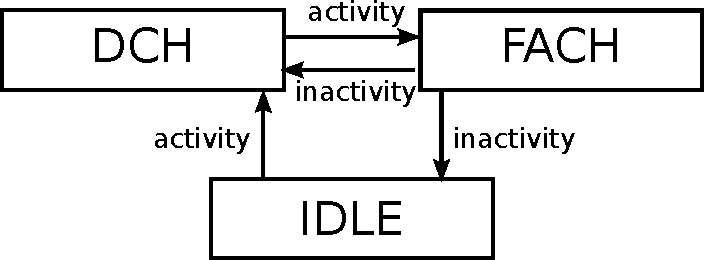
\includegraphics[width=0.8\columnwidth]{images/IMC2013/rrc-simplified-state-model.pdf}
	\caption{Simplified Radio Resource Control State Model.}
	\label{fig:rrcstatemodel}
\end{figure}


%%%%%%%%%%%%%%%%%%%%%%%%%%%%%%%%%%%%%%%%%%%%%%%%%%%%%%%%%%%%%%%%%%%%%%%%%%%%%%%%
\subsection{Discussion of GTP Signaling}

Looking at the Create, Update and Delete PDP Context Request and Reply message pairs we can already directly deduce some possibly load-related information. The total tunnel duration originates from the time delta between corresponding Create and Delete events. The shorter those tunnels are the higher will be volume of signaling messages and the necessary processing for these messages. Conversely, longer tunnel durations cause an increased overall memory footprint in the involved nodes to store the \ac{PDP} Contexts. Large numbers of update messages, especially combined with frequent \ac{RAT} switches, are usually an indicator for highly mobile devices switching their routing area. 
The time between a request and its corresponding response could also be an indicator for the amount of processing involved for this message as well as the current general processing load at the \ac{GGSN}.

As discussed, most of the actions in the network as well as in the mobile devices are reflected in the presented tunnel management messaging. Therefore, taking a look at the dynamics of this control aspect in real networks gives valuable insights on the influence of many of the networks' aspects.


%!TEX root = paper.tex
%%%%%%%%%%%%%%%%%%%%%%%%%%%%%%%%%%%%%%%%%%%%%%%%%%%%%%%%%%%%%%%%%%%%%%%%%%%%%%%
\section{Dataset and Methodology}
\label{sec:darwin-IMC}

For our analysis, we use the \ac{METAWIN} monitoring system developed in a previous research project and deployed in the network of an Austrian mobile operator.  More in-depth information about \ac{METAWIN} is available in \cite{ricciato_2011}.

 The location of the measurement probe at the Gn interface within the core network, marked in Figure~\ref{fig:umtsnetwork}, gives access to both wide-area mobility signaling (not analyzed in this paper) and signaling related to user-plane IP traffic (which we want to scrutinize). The \ac{METAWIN} monitoring system extracts and correlates information from the lower layers of the \ac{3GPP} protocol stack, and specifically the \ac{GTP} protocol on the Gn interface \cite{etsi_3gpp_2008}. This includes the \acf{RAT} identifier as well as the terminal types of the mobile clients. The latter is determinable by the \acf{TAC} part of the \acf{IMEI} (cf.~\cite{3gpp23003}) and will be discussed later in detail.

To meet privacy requirements, the \ac{METAWIN} system anonymizes captured data on the fly at multiple layers: the application-level payload is removed and all user identifiers (e.g. \ac{IMSI}) are hashed with a one-way function before recording. That is, single \acp{MS} in our dataset may be differentiated by means of an anonymized \ac{MS-ID}, but not traced back to the actual customer. The packet capturing hardware deployed within the \ac{METAWIN} monitoring system is synchronized using \ac{GPS}. Accordingly, the packet timestamps have an accuracy of $\pm100$ ns or better~\cite[p.97-98]{donnelly_high_2002}.

%%%%%%%%%%%%%%%%%%%%%%%%%%%%%%%%%%%%%%%%%%%%%%%%%%%%%%%%%%%%%%%%%%%%%%%%%%%%%%%%
\subsection{Dataset Description}

% TODO: more detailed data set description? maybe table? (# of entries etc)

%TODO: OLD
The \ac{METAWIN}-recorded dataset used in our evaluation is a week-long trace from the third week of April 2011. It consists of 2.2 billion aggregated flows for the user traffic and 410 million \ac{GTP} Tunnel Management transactions, the latter representing the data base for this paper. It was tapped at one of the \acp{GGSN} of the operator, and contains about half of the total traffic volume handled by the operator in this period. The \ac{GTP} data contains the response codes for each transactions. With these codes, failed interactions can be sorted out and treated separately.

We fed the records into a SQL database, and conducted further evaluations through scripted queries on the database. Any privacy-relevant data, e.g. the \ac{IMEI}, \ac{MS-ID} and any IP address involved, is only visible as hashes and is processed in a privacy-preserving manner.  Since the hashing of the \ac{IMEI} is consistent throughout the dataset, user traffic flows and the \ac{GTP} data can be cross-correlated despite anonymization, giving the opportunity for further research.


%%%%%%%%%%%%%%%%%%%%%%%%%%%%%%%%%%%%%%%%%%%%%%%%%%%%%%%%%%%%%%%%%%%%%%%%%%%%%%%
\subsection{Device Identification \& Classification}

Individual device types can also still be identified in form of the \ac{TAC} on every entry. The \ac{TAC} is part of the \ac{IMEI}, uniquely identifying each device type \cite{3gpp23003}. The rest of the \ac{IMEI} constitutes the serial number of the involved devices, which is not present in the data.

\acp{TAC} are managed by the GSM Association which in turn assigns local organizations, distinguished by the first two digits of the \ac{TAC} as Reporting Body Identifier, to allocate \acp{TAC} to manufacturers. However, this allocation information is not freely available. Commercial databases exist, but this is neither affordable for research institutions, nor is it conducive to our goal of providing information to the public. While there are some websites that allow one to query for specific \acp{TAC} for non-commercial purposes, only very few efforts attempt to collect \ac{TAC} information into a publicly available database. We based our data-mining efforts on a set from \cite{tacdb}, with some additional devices collected on our own. Since the unit identification part of the \ac{IMEI} is just six decimal digits long, popular devices will even be assigned more than one TAC, making the acquisition of all relevant \acp{TAC} even more complicated.

For our investigation, we went through large portions of the \acp{TAC} present in our dataset, and identified and categorized the most important entries. In this case, importance means various metrics like the traffic volume, the number of flows, and the number of \ac{GTP} signaling messages for each \ac{TAC}. 

After having available the device names for most \acp{TAC}, we were able to add meta-information and categorize the entries based on their device type and operating system. For the device type we partitioned the devices roughly into smartphones, regular mobile phones and 3G USB dongles or 3G/WiFi routers. The operating system includes most of the popular incarnations found in the network at measurement time, including Android, iOS, and Symbian. Note however that many devices, especially USB dongles cannot be linked to any specific OS.

\begin{table}
\centering
\caption{Relative \acs{TAC} Statistics.}
\label{tab:tacstats}
\begin{tabular}{|p{4cm}|p{3cm}|} \hline
& \textbf{Portion of devices with entry in TAC DB}\\ \hline
\# of Flows & 99.72\% \\ \hline
Ratio of Traffic & 99.97\%\\ \hline
\# of Tunnels & 87.57\% \\ \hline
\# of GTP Signaling Msgs & 90.95\% \\ \hline
\# of Distinct \acp{MS-ID} & 80.93\%\\ \hline
\end{tabular}
\end{table}

As we are working with an incomplete \ac{TAC} database it is important to know whether our \ac{TAC} mappings provide sufficiently useful data to allow for the envisioned device discriminating statistics. Therefore, Table~\ref{tab:tacstats} provides some statistics on our knowledge of devices in the dataset. About 80 percent of all distinct and active devices could be identified. Looking at the total number of \ac{GTP} signaling messages, we see that we can determine the device name of over 90 percent. The flow data shows an even clearer picture, as we can identify almost all of the devices involved.

After applying the categorization to the \acp{TAC} we evaluate the device composition in the network. The two largest portions of devices are smartphones and 3G dongles, while classic cell phones do not seem to play a major role in the packet-switched domain anymore. One observation across all device types is that about 14 percent of all mobile devices have activated their mobile data service and have signaling traffic, but do not cause any user plane traffic.

The difference between 3G dongles and smartphones is also noteworthy. While the former cause large amounts of user plane traffic (compared to the device numbers), they are responsible for but a few core network signaling events and tunnels. This picture is reversed for smartphones.


%!TEX root = paper.tex
%%%%%%%%%%%%%%%%%%%%%%%%%%%%%%%%%%%%%%%%%%%%%%%%%%%%%%%%%%%%%%%%%%%%%%%%%%%%%%%
\section{Core Network Load Statistics}
\label{sec:tunnelstats-IMC}

Having characterized the dataset available to us we now shed some light on the control plane and load dynamics in a mobile core network and attempt to show the possible impact of certain devices or other properties of the network. 


%%%%%%%%%%%%%%%%%%%%%%%%%%%%%%%%%%%%%%%%%%%%%%%%%%%%%%%%%%%%%%%%%%%%%%%%%%%%%%%%
\subsection{Defining Core Network Load}

Before beginning the evaluation, the primary question driving this investigation was: ``How can load in a core network be defined and measured?'' A summary of our thoughts to this question follows here.

With the basics of the architecture in mind, a top candidate for high load is the \ac{GGSN}. All traffic leaving or entering the packet switched domain must go through this element, and it is in control of the described GTP signaling procedures as well. Being an endpoint for the GTP tunnel makes it responsible to sort and encapsulate incoming traffic into the corresponding user tunnel. To accomplish this a lot of state has to be kept -- and processed when signaling occurs. Therefore, our working hypothesis is, that in order to determine load the \ac{GGSN} needs to be monitored closely and any traffic related to this node investigated for indications of the current load.

For our definition of the term ``load'' we differentiate between signaling load and overhead on the one hand and processing load and memory consumption on the other hand. Both are measures of load at specific nodes. While the former mostly has an impact on the actual network traffic, the latter can only be grasped inside the network element. With our data we can directly investigate the signaling traffic but indirect measures for the processing load and memory usage have to be found. In the rest of this section we evaluate the results of several approaches to both of these definitions of load.

While looking at the \ac{GGSN} may be the most obvious choice, it is by far not the only one. 
In addition to GTP tunnels the \ac{SGSN} has to handle \ac{RAB} and mobility management as well. However, it is assumed, that there are more regionally distributed \ac{SGSN} nodes present in a typical mobile network. This means that a single element would have to handle less mobile devices and therefore load. One has also to bear in mind that the \ac{SGSN} can be completely circumvented by setting up a direct tunnel between \ac{GGSN} and \ac{RNC}.

Apart from the two gateways directly inside the traffic path there are several other nodes essential to the control plane decision making, which may very well be also very load-sensitive. The \ac{HLR} for example is a central database storing all user related information which need to be retrieved any time a user needs to undergo initial authentication and authorization. Typically, the procedures the elements are involved in are fewer and they are also harder to investigate with the data available to us. Hence, it was decided to concentrate just on the case of the \ac{GGSN}.


%%%%%%%%%%%%%%%%%%%%%%%%%%%%%%%%%%%%%%%%%%%%%%%%%%%%%%%%%%%%%%%%%%%%%%%%%%%%%%%
\subsection{Load Influencing Factors}
% TODO: OLD, WAS: \subsection{Factors Influencing Tunnel Durations}

Having described our understanding of core network load we can now move to discuss some of the factors that could influence the load, making them targets for our evaluation.

The first and arguably one of the most important factors are the mobile devices themselves. Specifically, this covers the behavior of the network layer 1 and 2 implementation (sometimes called ``'baseband'') as well as the \ac{OS} and the running applications. The OS and baseband decide when the device should establish a mobile data connection, how long the connection is held, or which mobile technology takes preference. Depending on the access technology, be it \acs{GPRS}, \acs{EDGE}, \acs{UMTS}, \acs{HSPA}, or \acs{HSPA+}, we can expect subtle differences through their specifications, e.g. in the timing of the radio transmission intervals, which could influence our investigation. 

Some specific tunnel duration properties could stem from the \ac{OS}'s IP and transport protocol implementation. For example, TCP timeouts might be configured to different default values causing mobile connections and tunnels to be held either shorter or longer. Also, mobile network firewalls have been found to interfere with transport and application layer timeout and keep-alive or heartbeat mechanisms on mobile devices \cite{sigcomm11middleboxes}.

The actual user-traffic patterns are generated by the applications running atop the OS. An example for how applications can influence network signaling is the aforementioned ``Angry Birds'' with its ad-retrieval strategy causing network traffic and possibly signaling in certain intervals. Since the application ecosystem for smartphones is extremely rich and ever growing we cannot pinpoint individual ones from our aggregate dataset.

An additional factor in the picture is the user and her or his behavioral patterns. They express themselves both in the traffic dynamics and in the mobility pattern, but they are rather difficult to distinguish in such a dataset given the large amount of data and the difficulty of correctly correlating tunnel management messages. We leave this as potential future work.

Easier to observe are the temporal effects of user behavior, which do not target individual users but the overall effects of a device's usage based on the time of day, the day of the week, or other time spans. In network user traffic analyses diurnal effects are typically very distinct with peak traffic some time during the day and the lowest traffic shortly after midnight. But these investigations are for user traffic only. We aim to find out, if the mobile network control plane shows similar patterns and can thusly be correlated to user traffic.

We also expect the mobile network and its protocol implementations to express themselves in the measurements. For example, the \ac{RRC} idle timer is typically in the range of 10 to 30 minutes, which could mean there will be a large number of tunnels with a duration in this range. Such choices are usually made either by the mobile network operator or the device manufacturer and can vary from one implementation to another. It is therefore quite difficult to give any hard numbers in advance, and one has to correlate such aspects with certain events in the results.



%%%%%%%%%%%%%%%%%%%%%%%%%%%%%%%%%%%%%%%%%%%%%%%%%%%%%%%%%%%%%%%%%%%%%%%%%%%%%%%
\subsection{Individual Examinations}

To examine some of these factors, we present the following number of individual investigations. Our measure of choice are the GTP tunnels as they carry lots of meaning in being directly related to the signaling amount in the network. We investigate their duration as well as the number of arrivals and look at a measure for the processing time of events at the GGSN. These insights will also allow us to build a simple toy model for the core network load in the next chapter.


%%%%%%%%%%%%%%%%%%%%%%%%%%%%%%%%%%%%%%%%%%%%%%%%%%%%%%%%%%%%%%%%%%%%%%%%%%%%%%%
\subsubsection{GTP Tunnel Duration}

In our evaluation, we define the duration of a GTP tunnel as the time between a GTP CREATE and the corresponding GTP DELETE event. After the reply for a CREATE has been sent from the \ac{GGSN} any setup procedures at the node should have completed and it should recognize incoming traffic from or to this user. After the DELETE, the user's traffic will not be routed anymore. Any lazy cleanup happening after the DELETE is not relevant for this specific investigation.

We differentiate all the tunnel events in our dataset based on two factors. First, we look at tunnels from different device types, be it either a smartphone, a regular or feature phone, or one of the many 3G dongles or mobile routers. After that, we investigate possible influences from the operating system. Both categorizations should prove valuable for example in deciding if currently some phone types put more signaling load on the network and to direct measures to improve this situation.



%%
\paragraph{Influence of the Device Type}
%%

\begin{figure}
	\centering
	\includegraphics[width=\columnwidth]{images/IMC2013/tunnel-dur-class-cdf-mod.pdf}
	\caption{Tunnel duration distribution, separated for 3G dongles, smartphones and regular phones with medians at 115s (Total), 31s (Regular), 82s (Smartphone), and 1207s (3G Dongle)}
	\label{fig:cdf-duration-device-class}
\end{figure}

Figure~\ref{fig:cdf-duration-device-class} shows the empirical cumulative distribution functions for the PDP Context durations in our dataset. We distinguish the total duration distribution as well as the the distributions for smartphones, regular phones, and 3G dongles. It can be observed that tunnel durations range between mere seconds and more than one week\footnote{Although our dataset is just one week long, some tunnels started before the beginning of that week, and ended within it. Since the tunnel start dates were still available from the system, we chose to include the data.}.

The median is clearly different between device types, being much longer for 3G dongles than for mobile phones. This can probably be expected, as typical dongle sessions might involve working at a laptop for periods longer than a few seconds or minutes. Also, for the dongles, we observe less extremely long tunnels. Again, we could relate this to a hypothetical laptop working environment, where the device is used for a few hours but then shut down. With this, the PDP Context is deleted as well. 

Interestingly, the median duration of regular phones is higher than that of smartphones. This may indicate that smartphones regularly (and perhaps automatically) cause data traffic and therefore tunnels to occur. We conjecture this to be a first indication of the ``Angry Birds'' effect of automatically transferring small amounts of data, e.g. weather reports, stock exchange data, RSS feeds, or email notifications. We also observe two distinct steps, one at 6.8 seconds for dongles, and one at 30 minutes in the overall and smartphone distributions.


%%
\paragraph{Influence of the OS}
%%

\begin{figure}
	\centering
	\includegraphics[width=\columnwidth]{images/IMC2013/tunnel-dur-os-cdf-mod.pdf}
	\caption{Tunnel duration cumulative distribution function, separated for Android and iOS devices; Medians at 115s (Total), 15.5s (Symbian), 104s (iOS), and 765s (Android)}
	\label{fig:cdf-duration-os}
\end{figure}

Taking an even closer look at the smartphone device fraction, and differentiating the operating system to Symbian, Android, and iOS, we can still observe major differences as depicted in the empirical cumulative distribution functions of Figure~\ref{fig:cdf-duration-os}. The tunnel duration distribution of the Symbian device fraction behaves much closer to the regular phones already depicted in Fig.~\ref{fig:cdf-duration-device-class}. A possible explanation could be the user-base being more traditional, or the devices being feature phones whose behavior clearly differs from smartphones.

Again, a number of steps (i.e. accumulations of incidents) are visible in the distributions. Those that are only visible in one operating system type point to a source involving the device rather the network. This especially includes the 30 seconds, 300 seconds, and 600 seconds steps for Android, and the 600 seconds step for iOS devices. However, whether this behavior should be attributed to the operating systems themselves cannot be decided by only looking at these distribution. Other sources, e.g. the device's firmware version and user traffic dynamics need also be observed.

A last artifact of note are the large number of iOS devices with very short tunnel durations. Over 20\% of all tunnels established by these devices are shorter than two seconds. Our working hypothesis is, that this is an interaction between short regular traffic burst and a form of Fast Dormancy \cite{gsma2011fdbestpract} which iOS devices are known to implement, a technique to explicitly release radio resources. It is deemed to improve device battery life, radio signaling and radio spectrum efficiency. However, due to the earlier and more frequent radio state changes, it also could cause an increase in core network tunnel management signaling, which is probably what happened in the iOS case depicted in the CDF.



%%%%%%%%%%%%%%%%%%%%%%%%%%%%%%%%%%%%%%%%%%%%%%%%%%%%%%%%%%%%%%%%%%%%%%%%%%%%%%%
\subsubsection{Tunnel Number of Arrivals and Inter-Arrival Time}

While tunnel durations and the involved signaling at the beginning and end of the duration is one aspect of control plane load, the number of tunnel arrivals might be another, which we are looking into in this section.

In addition to describing the arrival process on the basis of the number of arrivals, we also take a look at the tunnel inter-arrival time. Specifically, with this process we mean the arrival of tunnel requests, i.e. GTP CREATE requests, at the \ac{GGSN}. This also adds to the foundation of the load model constructed in the next chapter. 

\begin{figure}
	\centering
	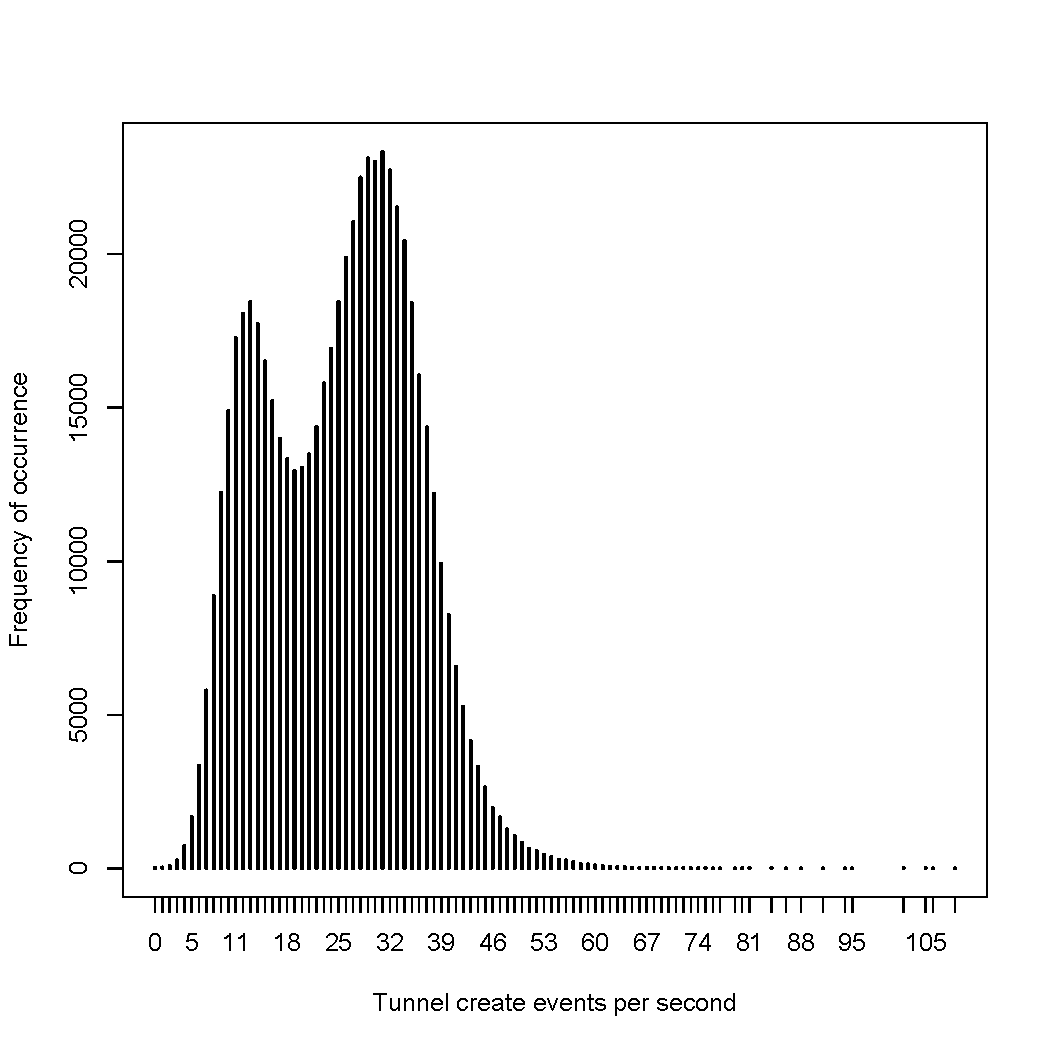
\includegraphics[width=\columnwidth]{images/IMC2013/create_freq.pdf}
	\caption{Tunnel arrivals in one second intervals.}
	\label{fig:freq-arrivals}
\end{figure}

Figure \ref{fig:freq-arrivals} depicts the number of arrivals per second during the whole weeklong period. Of note is the clear bimodal nature with one peak around twelve and the other in the low thirties. While the distribution is rather compact around these two peaks, there are some clear outliers up to 107.
If we again hypothesize that an increased number of arrivals means higher load in the network, we can assume that load is not constant but rather switches between two modes with some periods with extraordinary load induced by an increased number of arrivals.

\begin{figure}
	\centering
	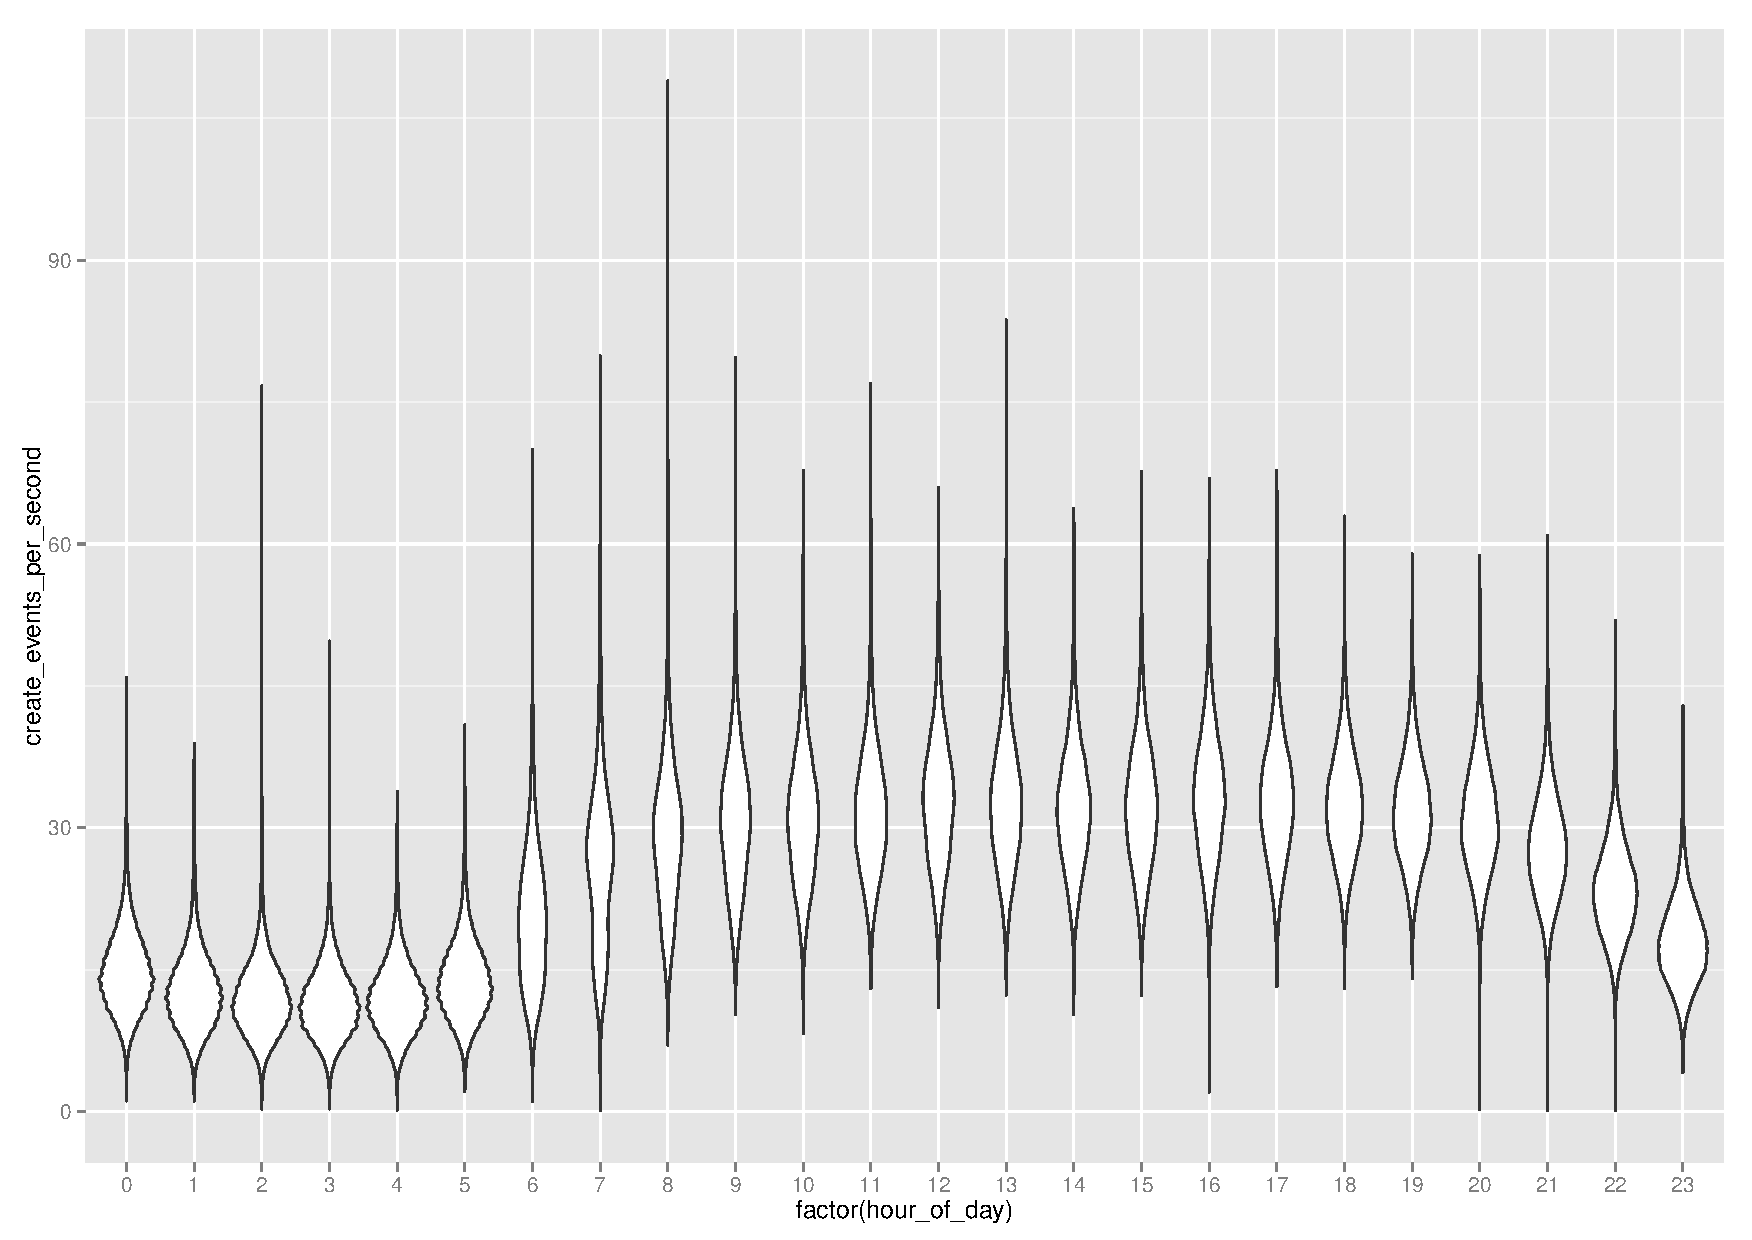
\includegraphics[width=\columnwidth]{images/IMC2013/R-createspersecond-1h-violin.pdf}
	\caption{Violin plot of tunnel arrivals in one second per time of day.}
	\label{fig:freq-arrivals-per-second-violin}
\end{figure}

To find the cause of these two modes we take a peek at the diurnal arrival pattern. Figure \ref{fig:freq-arrivals-per-second-violin} contains a violin plot showing again the arrivals per second but broken down by time of day. A violion plot, while being similar to a box plot, additionally shows the density of the individual items on the vertical axis.
The nocturnal median from around midnight to 5am and the longer daytime median, 8am to 19pm, closely resemble the two modes found in the histogram. In between are short transition phases. Notably, during daytime the arrivals and their densities are spread out on a much larger value range. This could be an indication of load fluctuations in the system.


\begin{figure}
%\vskip -2.5cm
        \centering
        % \begin{subfigure}[b]{0.50\textwidth}
        %         \centering
        %         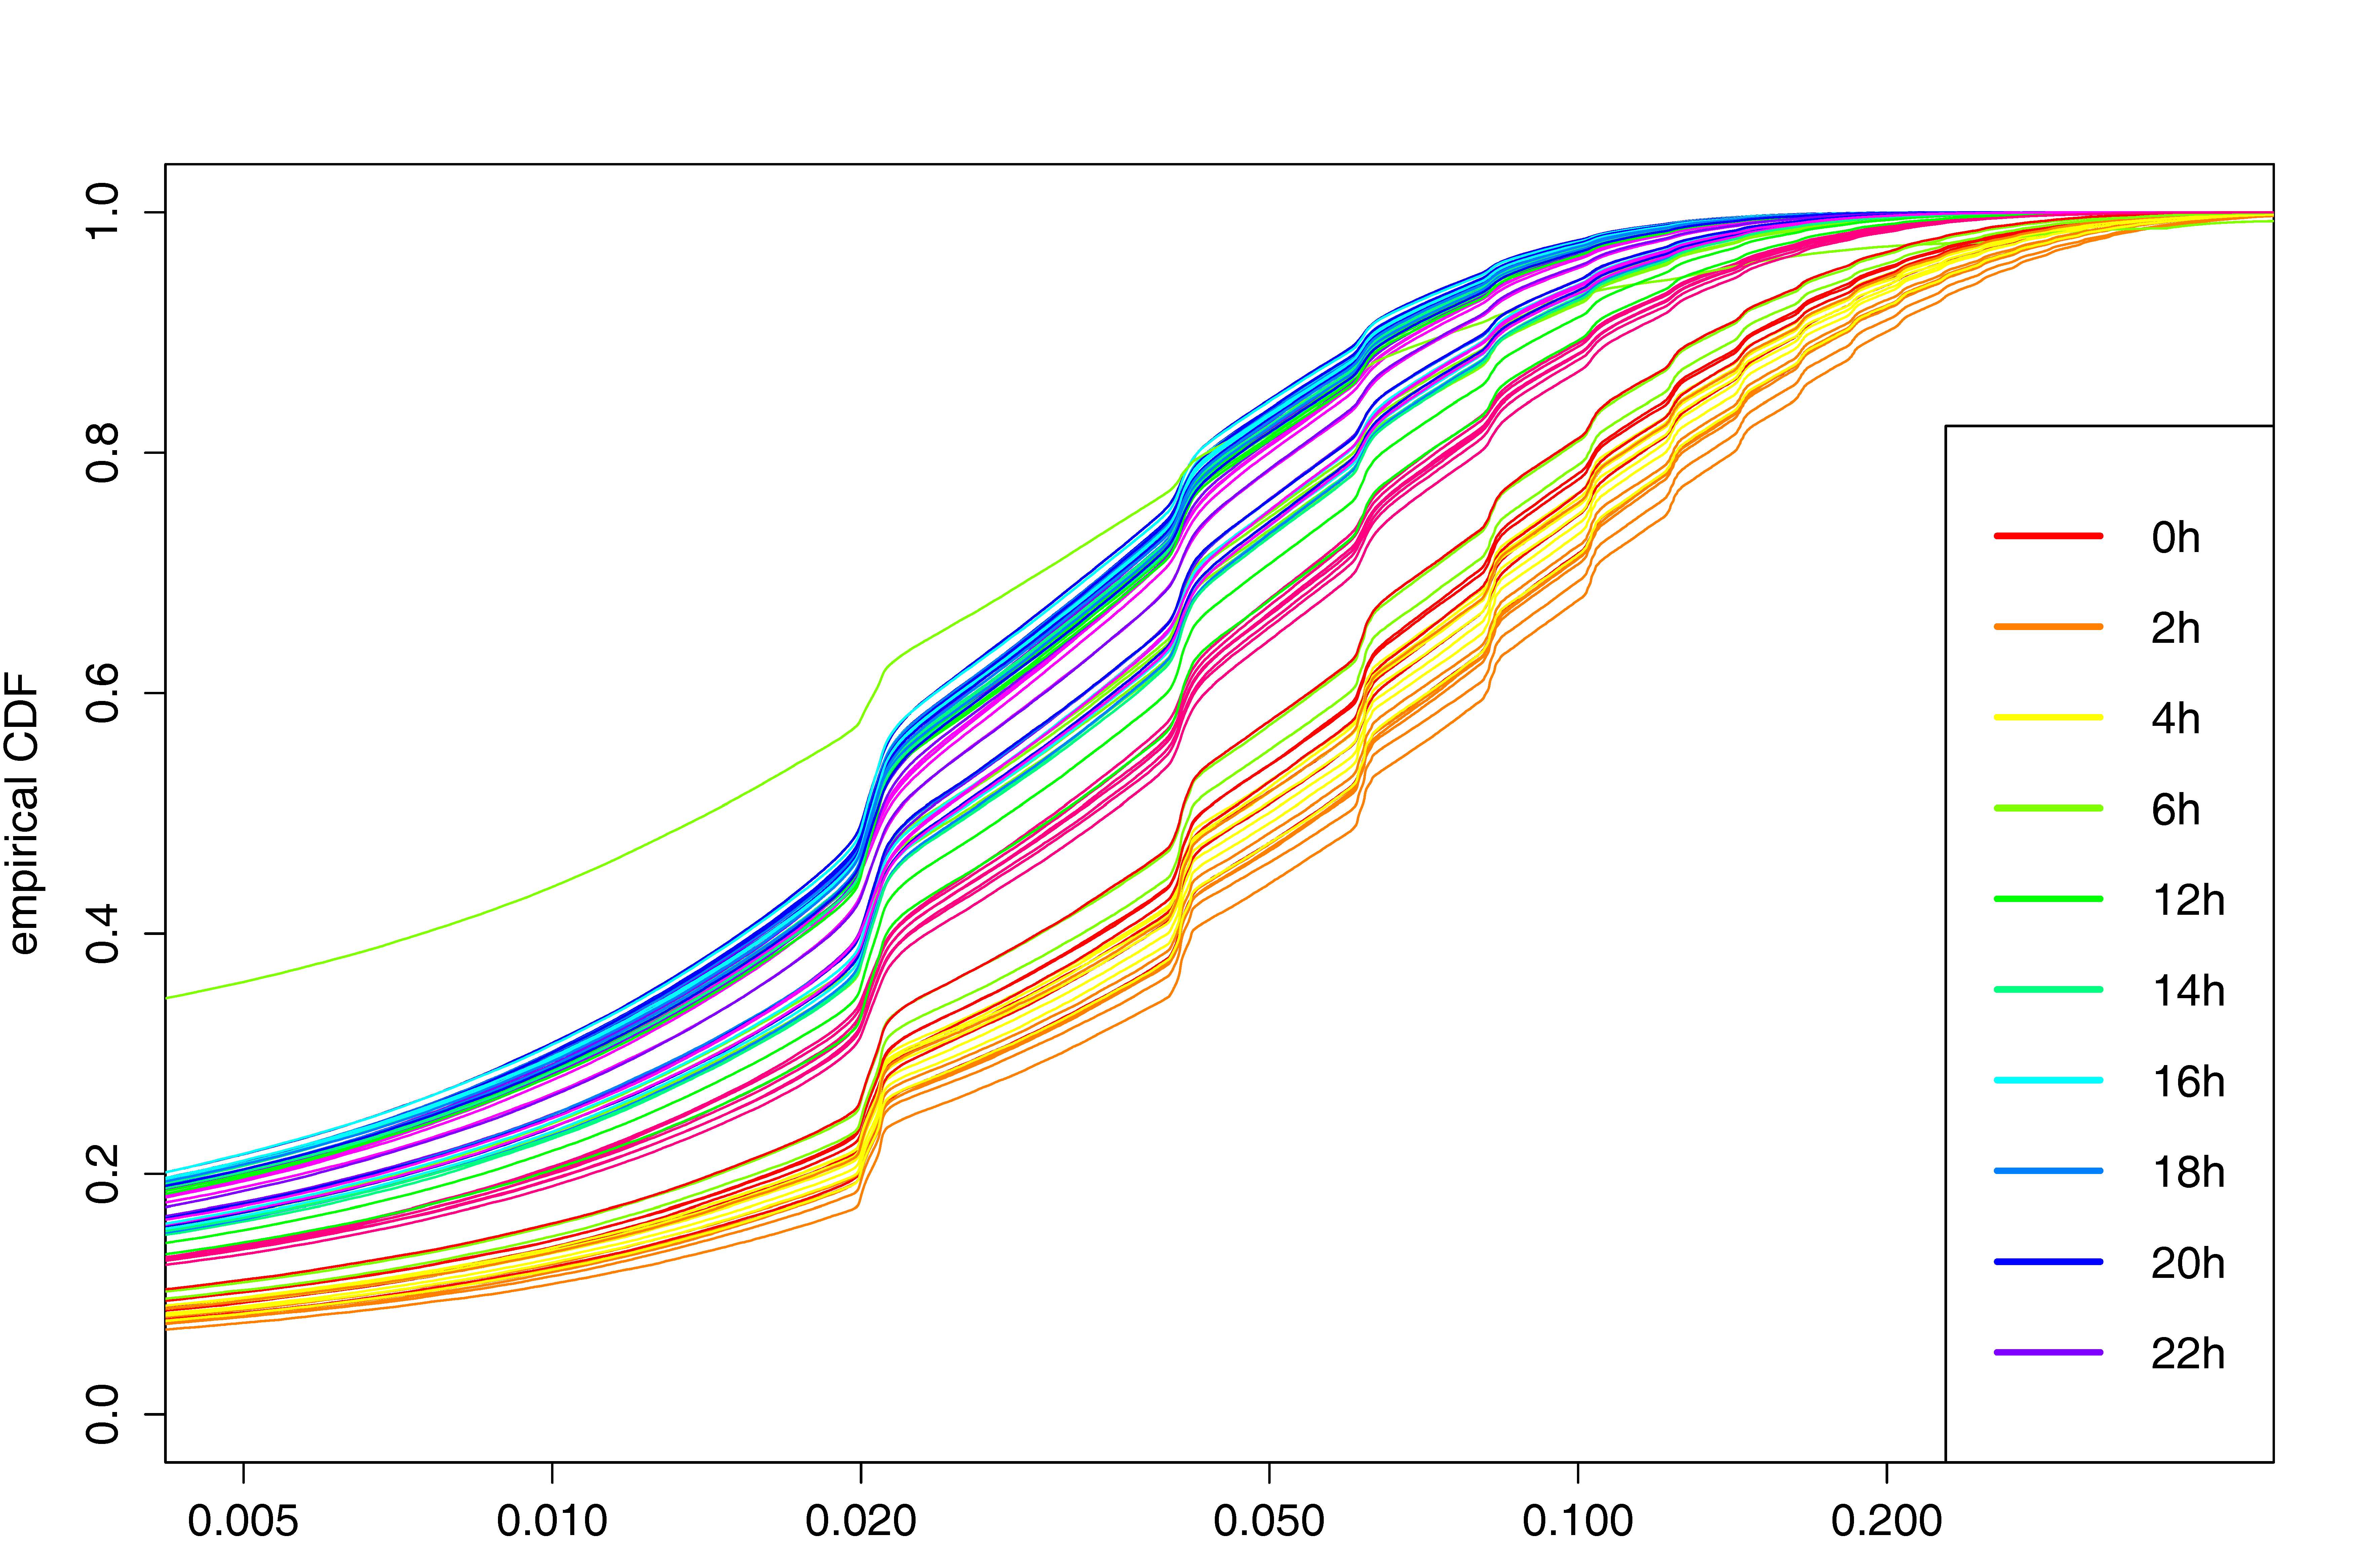
\includegraphics[width=\textwidth]{figures/R-IAT-ecdf-2h-log.png}
        %         \caption{All incoming tunnel requests.}
        %         \label{fig:IAT-ecdf-2h-all}
        % \end{subfigure}%
        %~ %add desired spacing between images, e. g. ~, \quad, \qquad etc.
          %(or a blank line to force the subfigure onto a new line)
        \begin{subfigure}[b]{0.50\textwidth}
                \centering
                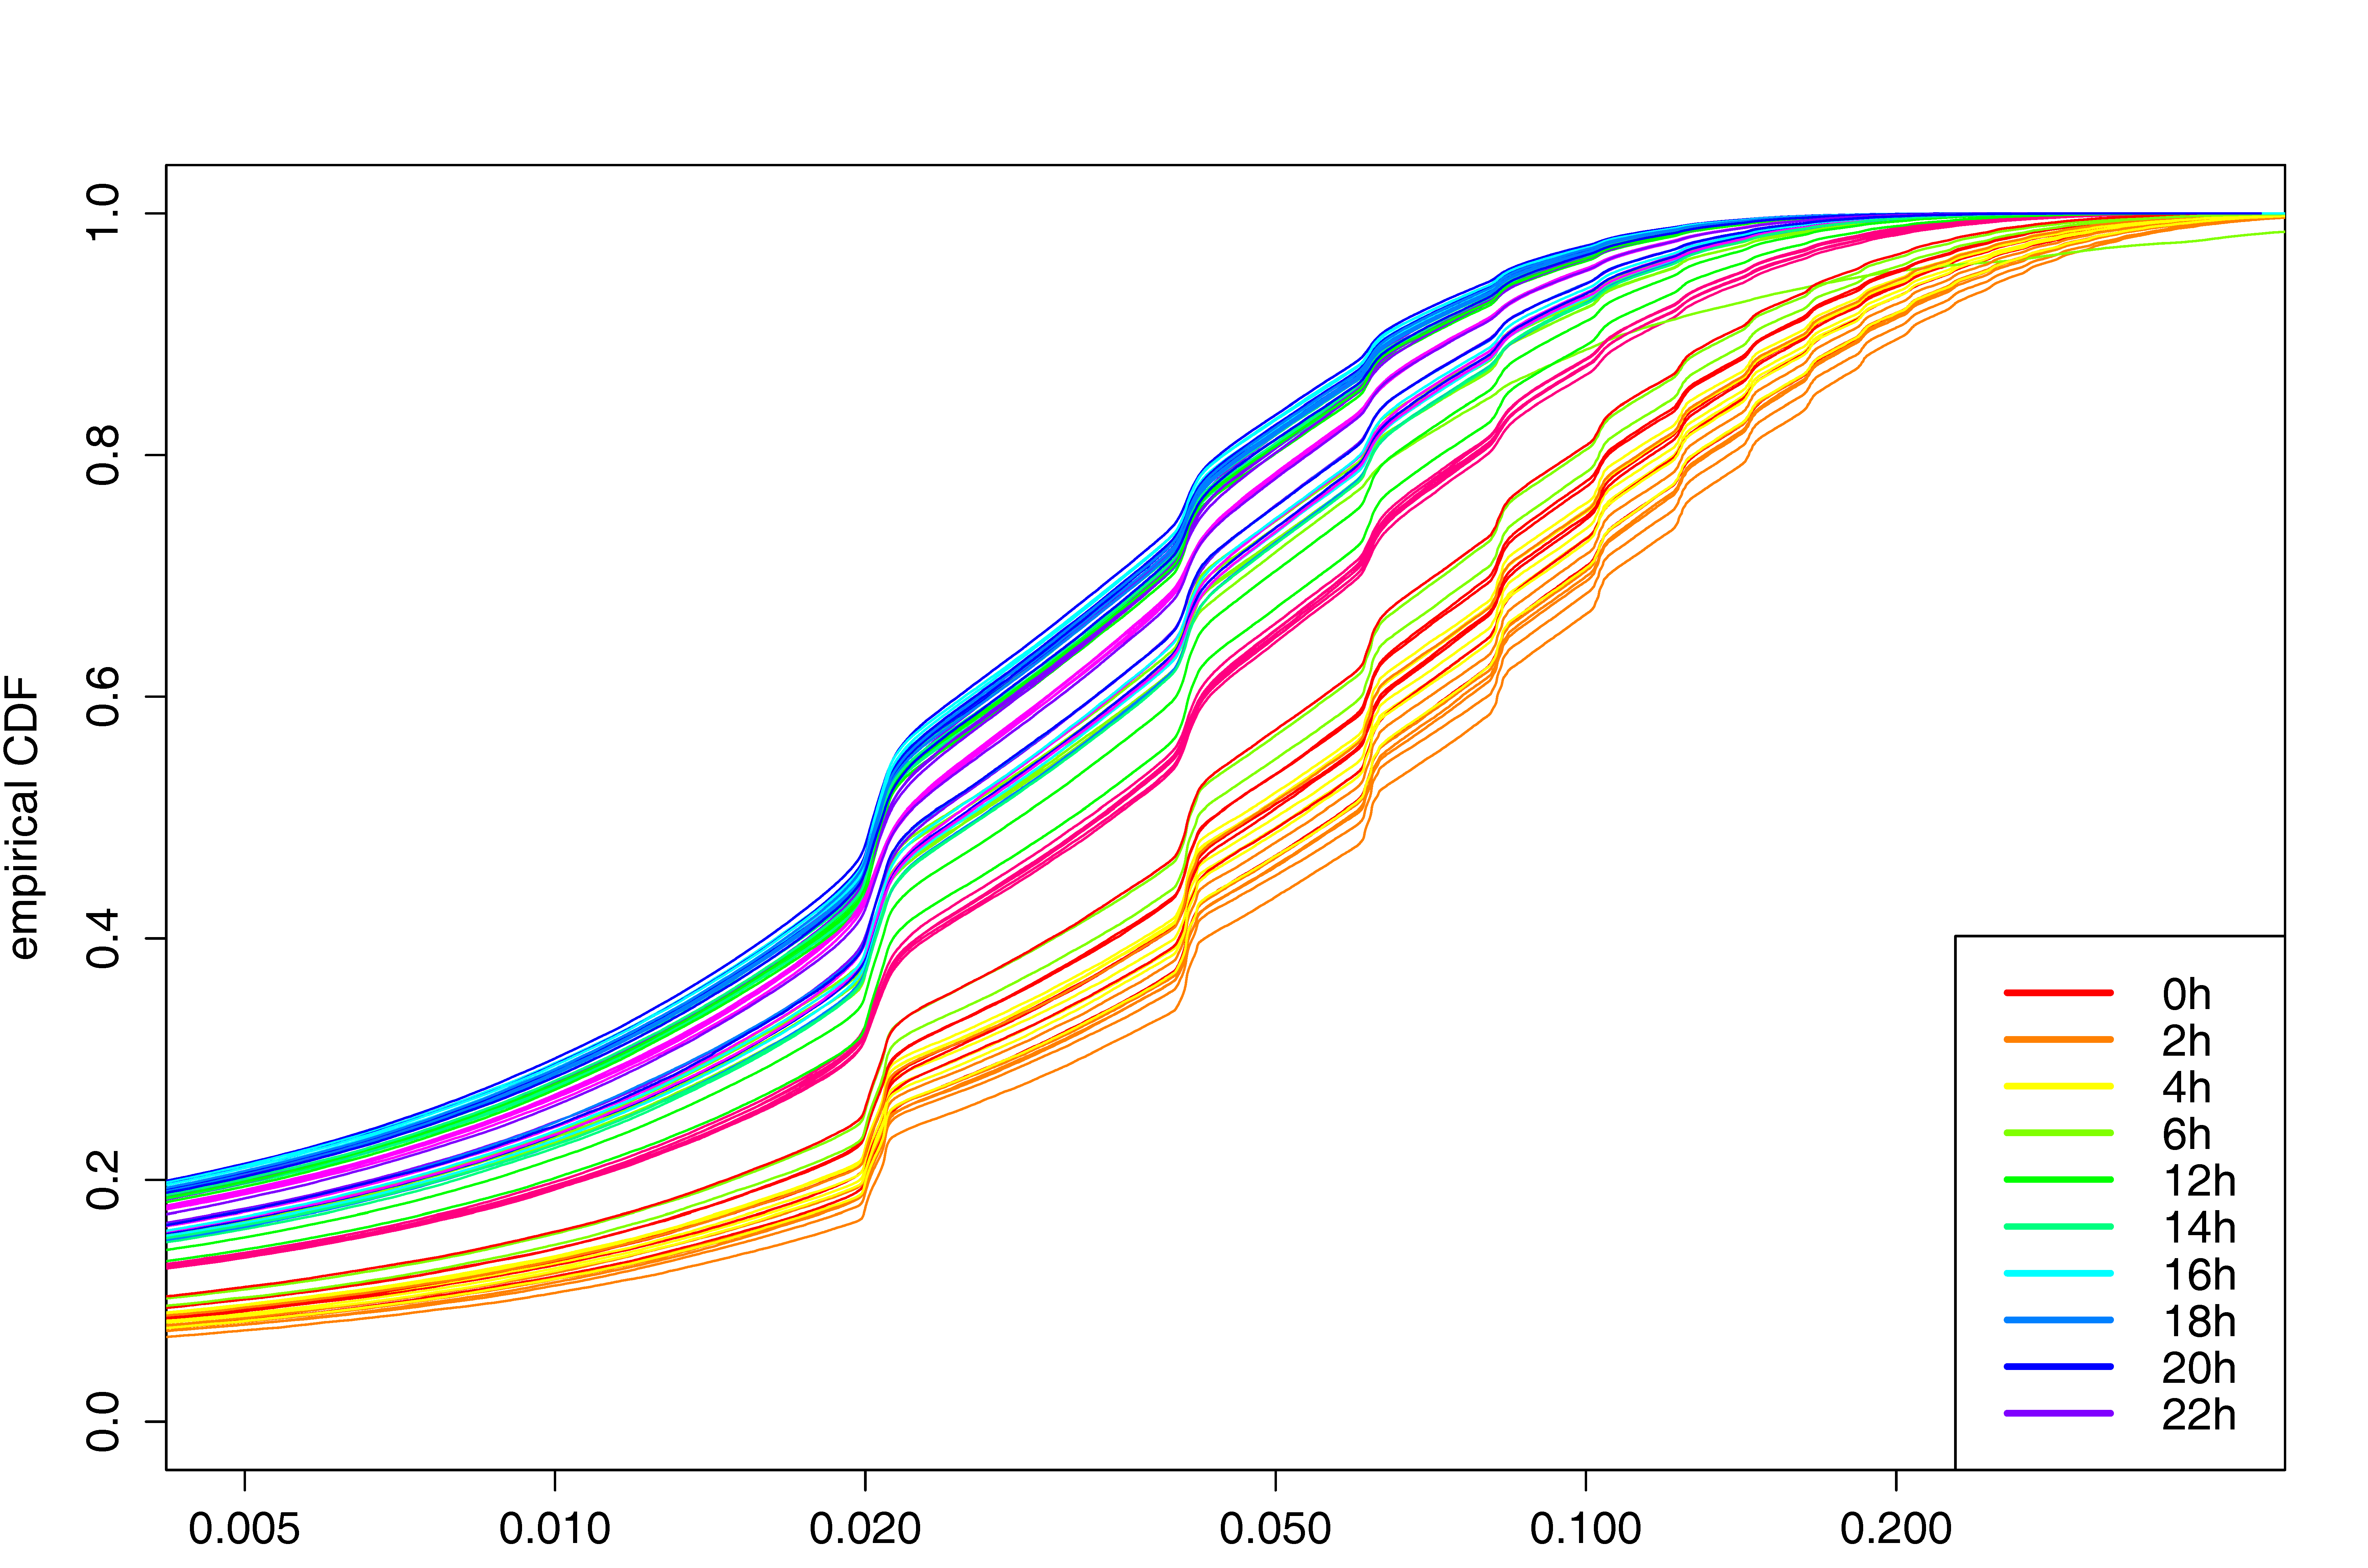
\includegraphics[width=\textwidth]{images/IMC2013/R-IAT-successful-2h-ecdfs.png}
                \caption{Successful tunnel requests.}
                \label{fig:IAT-ecdf-2h-successful}
        \end{subfigure}%
        ~
        \begin{subfigure}[b]{0.50\textwidth}
                \centering
                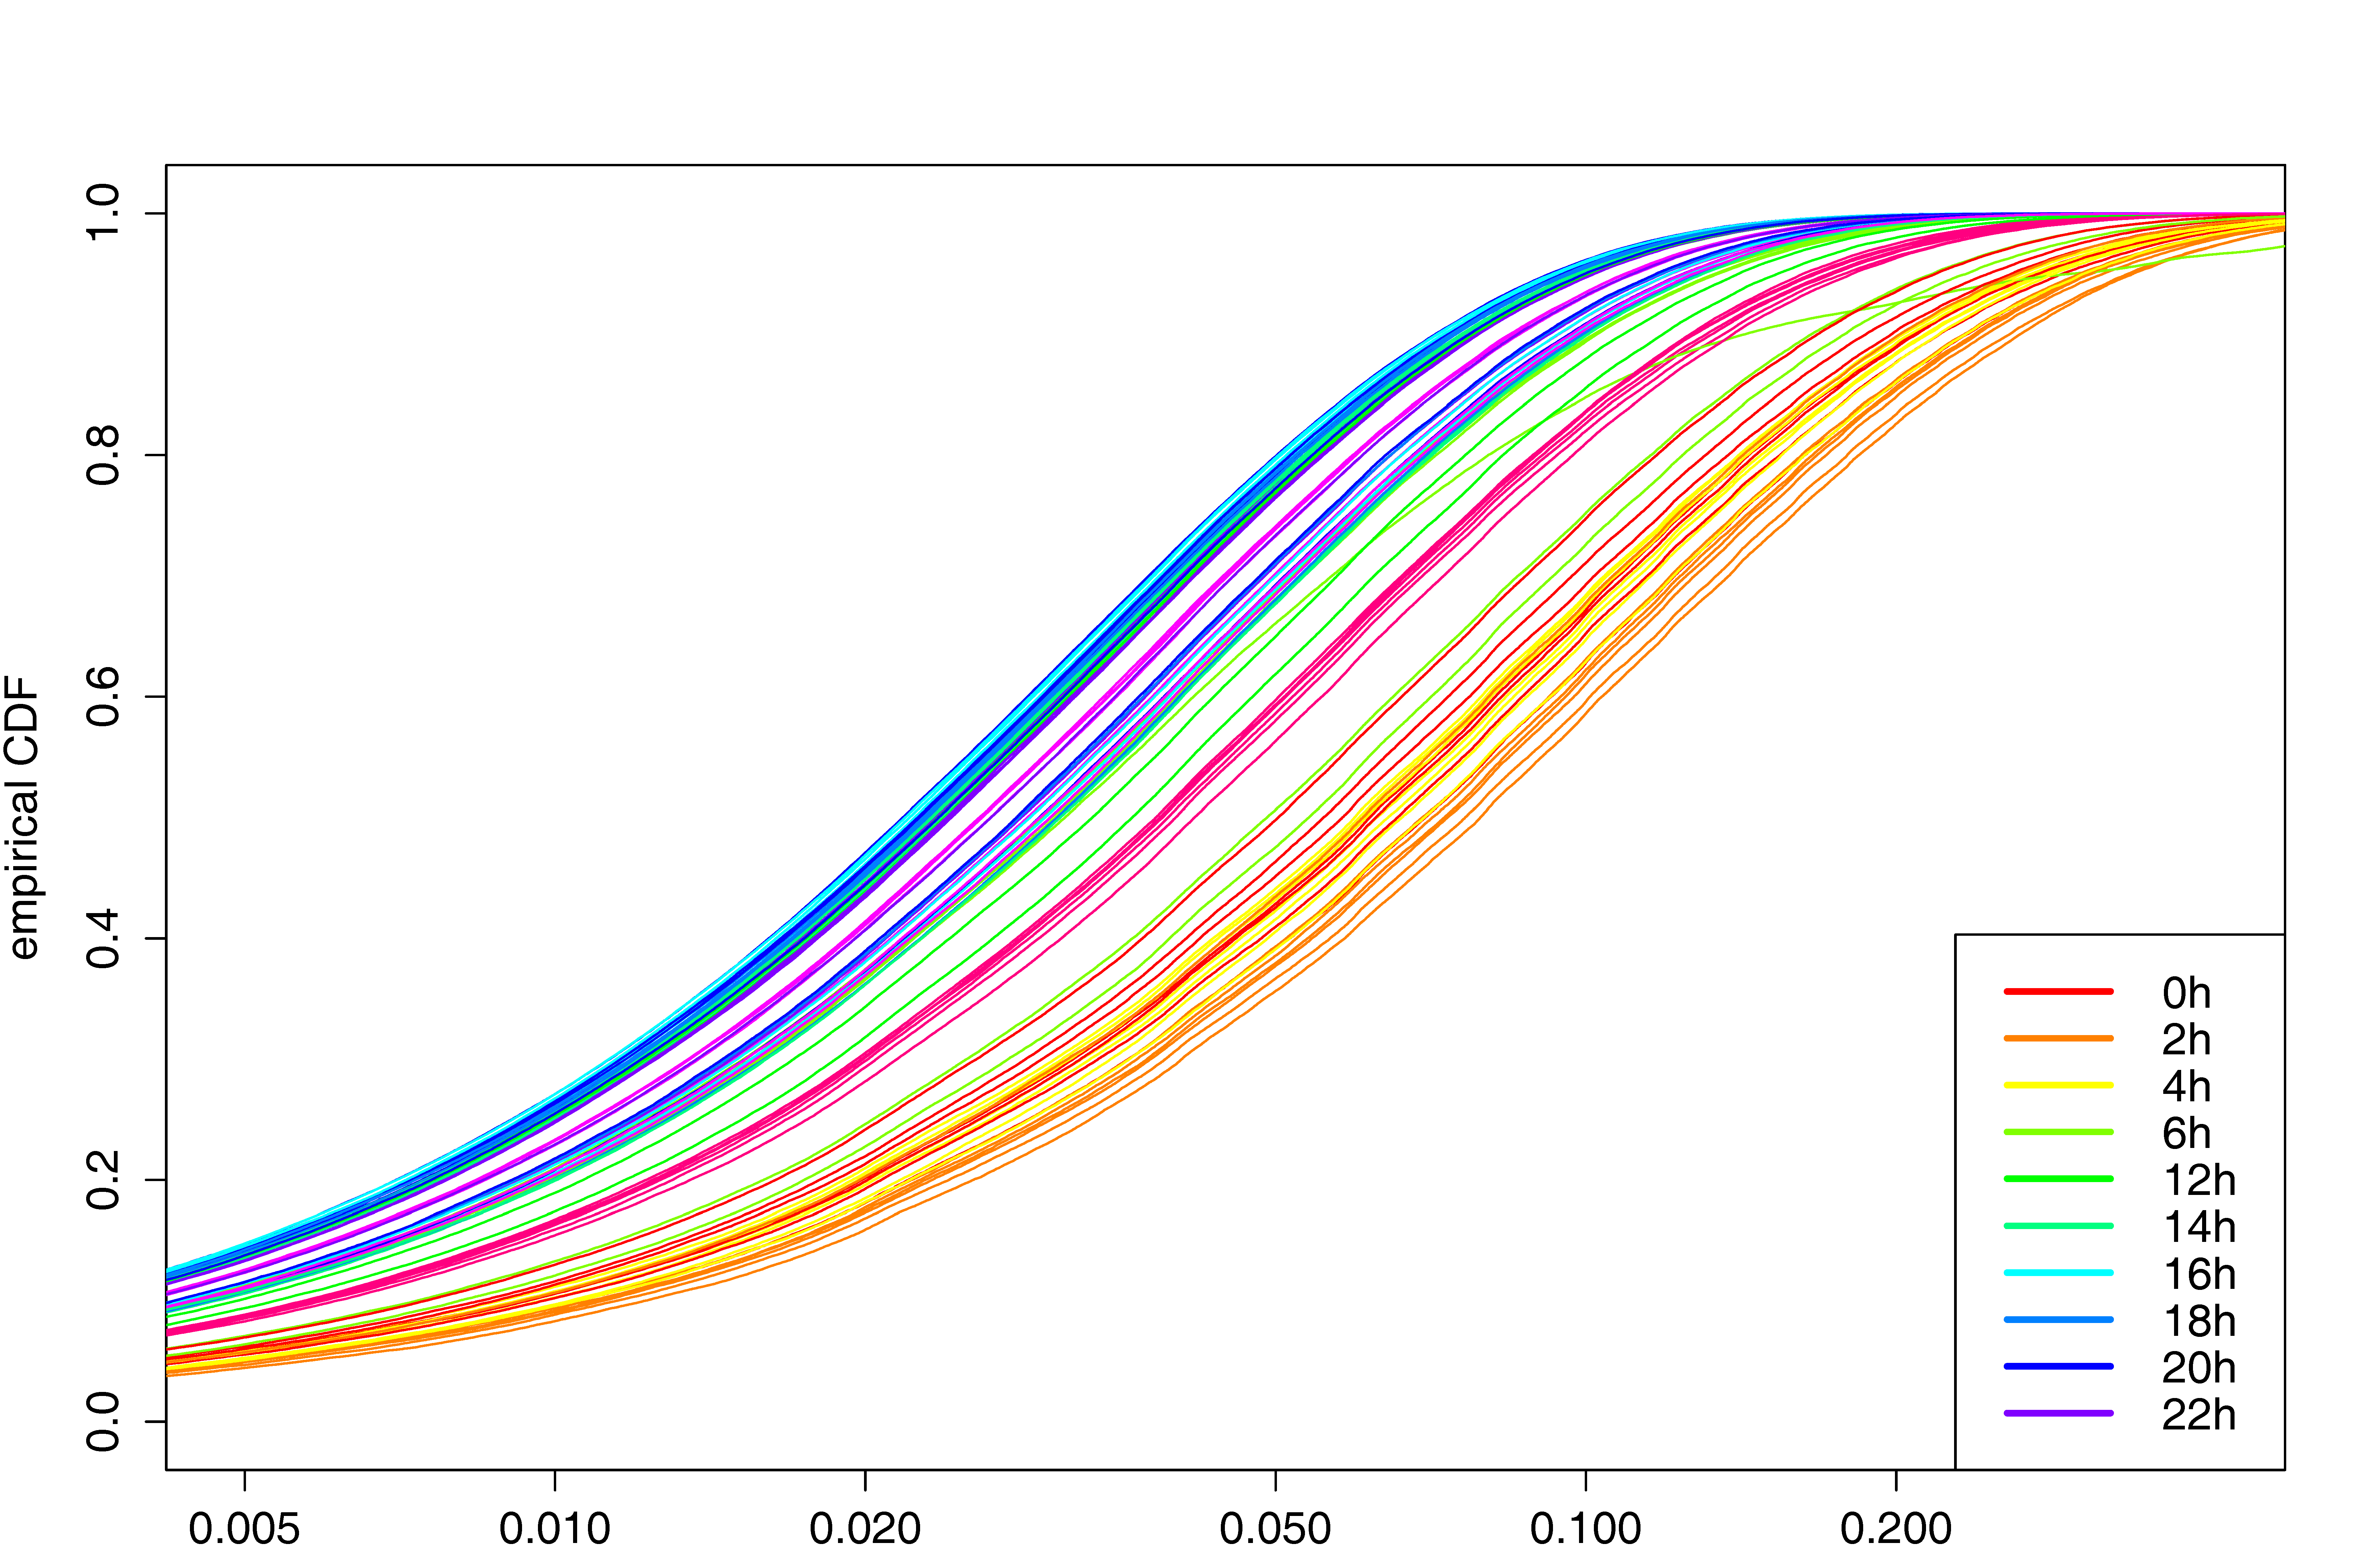
\includegraphics[width=\textwidth]{images/IMC2013/R-IAT-fromflows-ecdfs-2h.png}
                \caption{Only tunnels with data flows.}
                \label{fig:IAT-ecdf-2h-active}
        \end{subfigure}
        
        \begin{subfigure}[b]{0.50\textwidth}
                \centering
                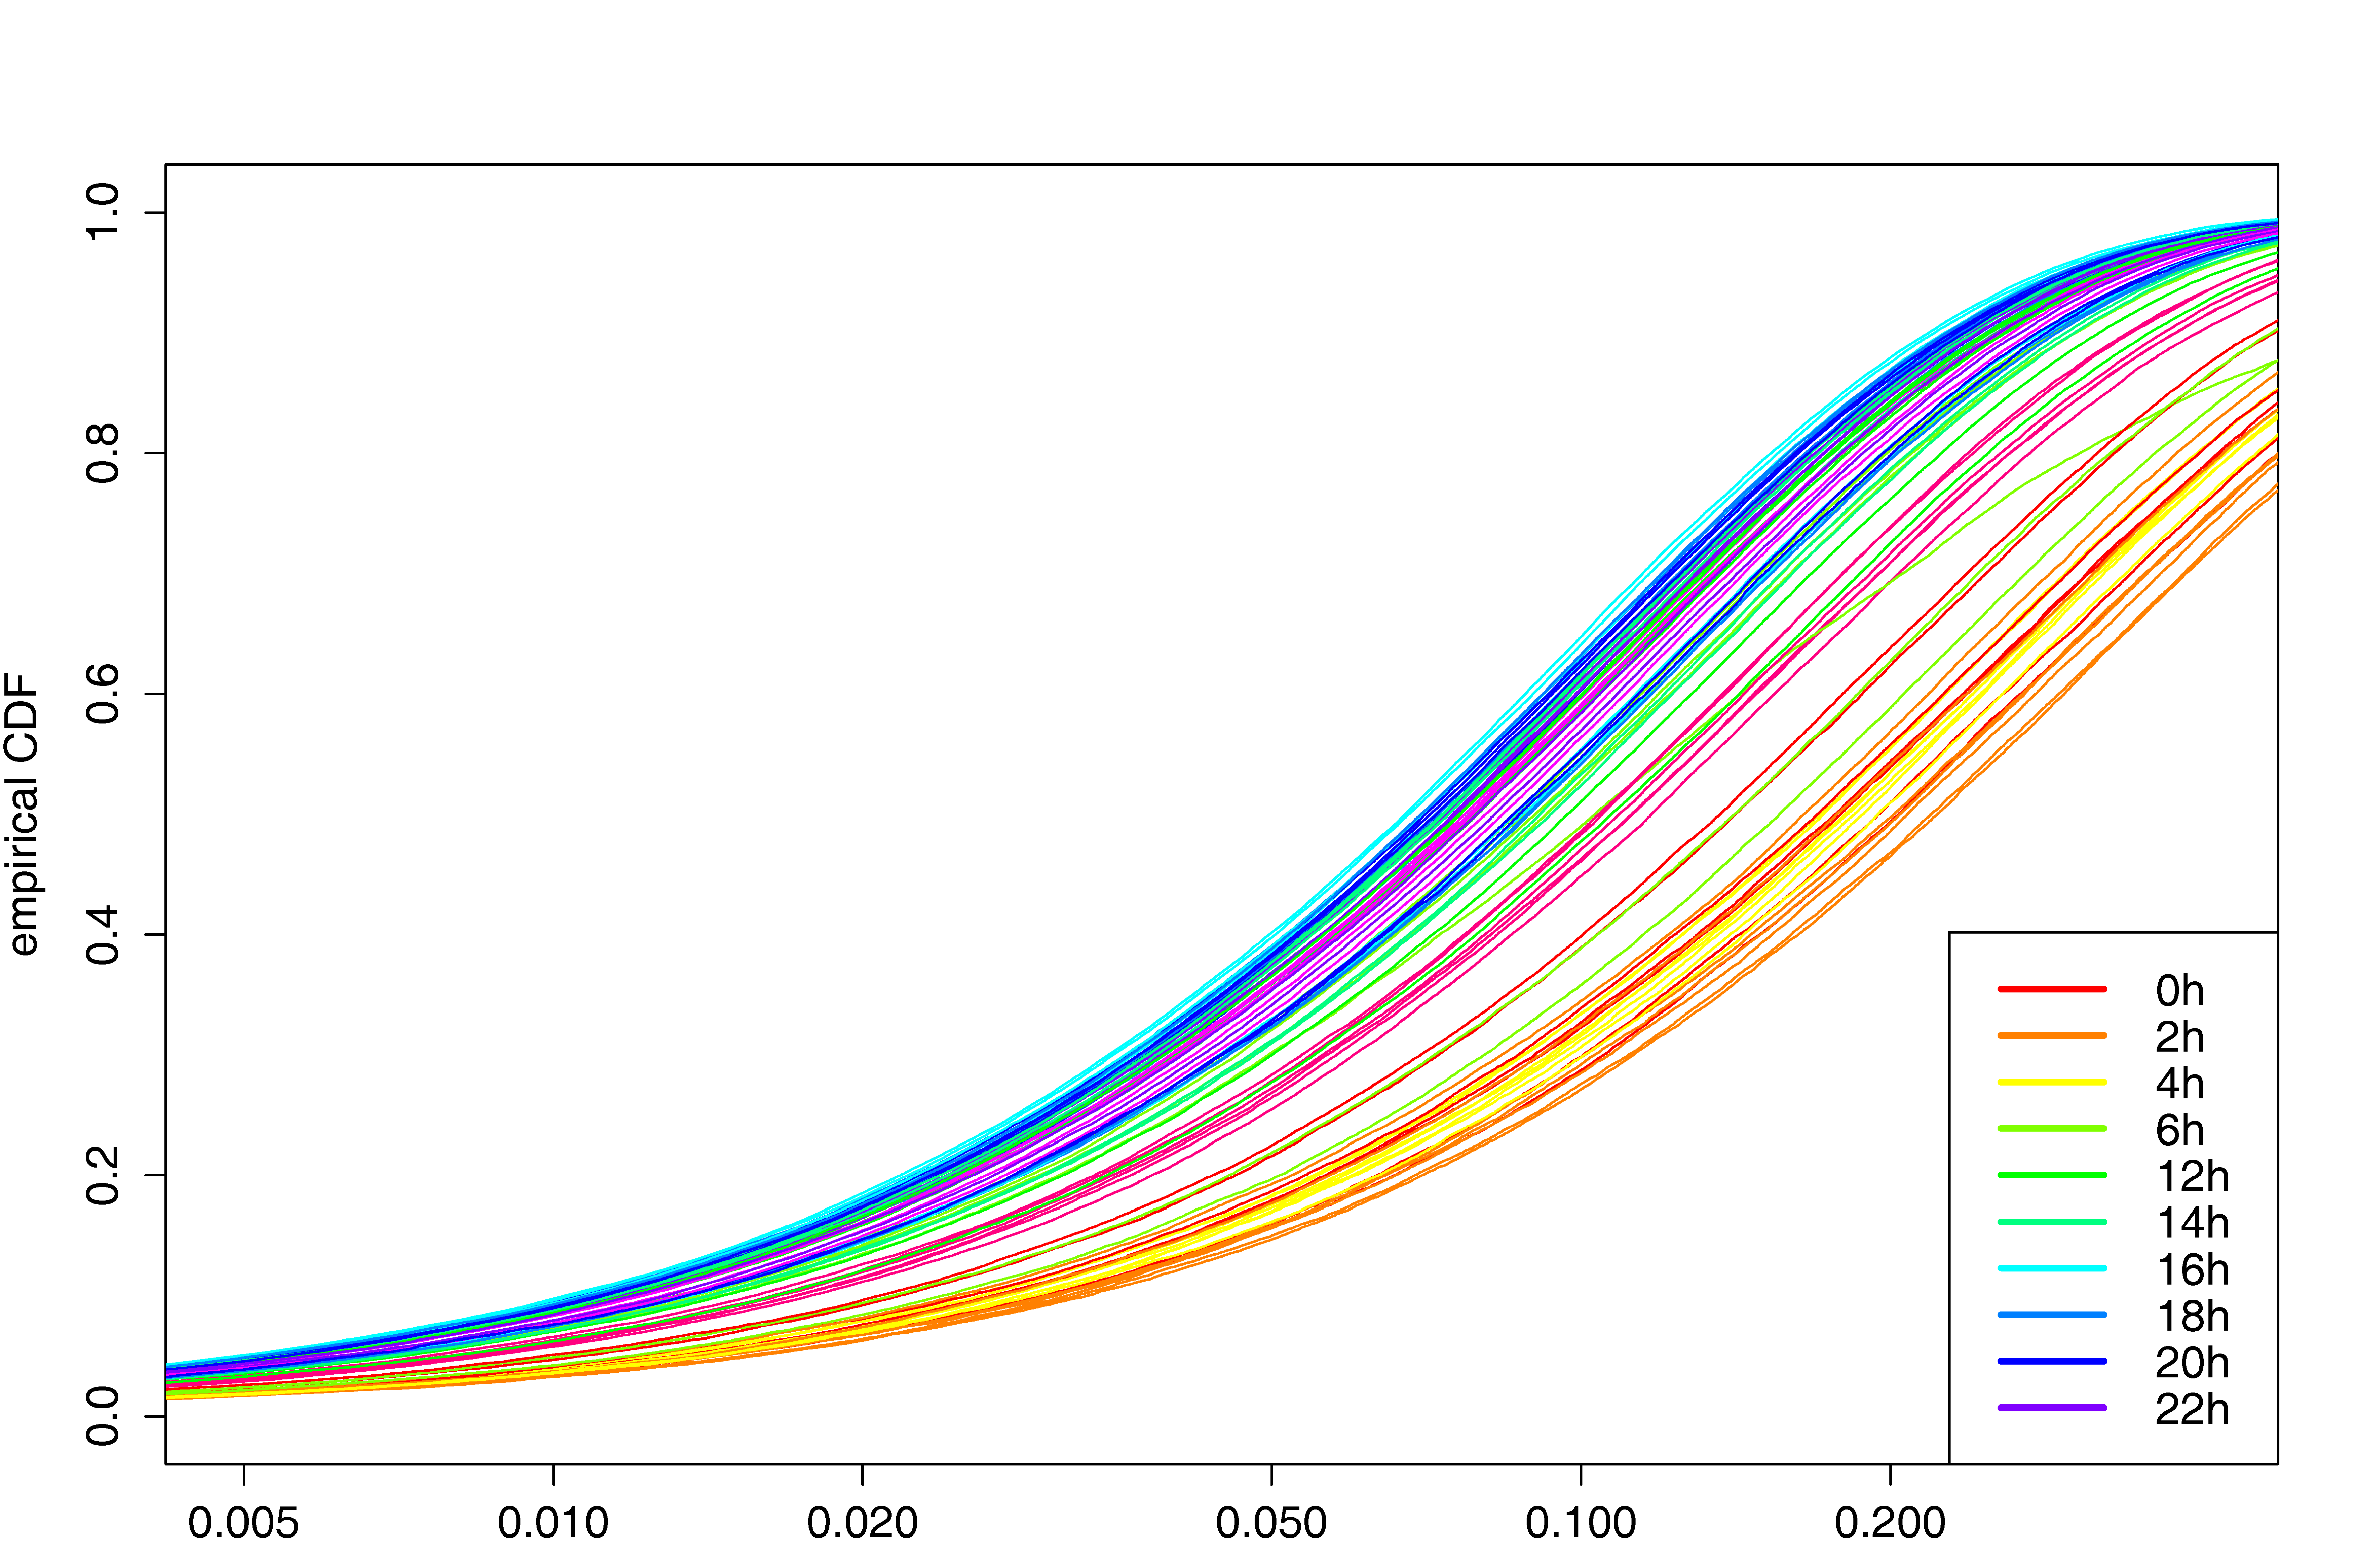
\includegraphics[width=\textwidth]{images/IMC2013/R-IAT-fromflows-gprs-ecdfs-2h.png}
                \caption{Only GPRS tunnels with data flows.}
                \label{fig:IAT-ecdf-2h-active-gprs}
        \end{subfigure}%
        ~
        \begin{subfigure}[b]{0.50\textwidth}
                \centering
                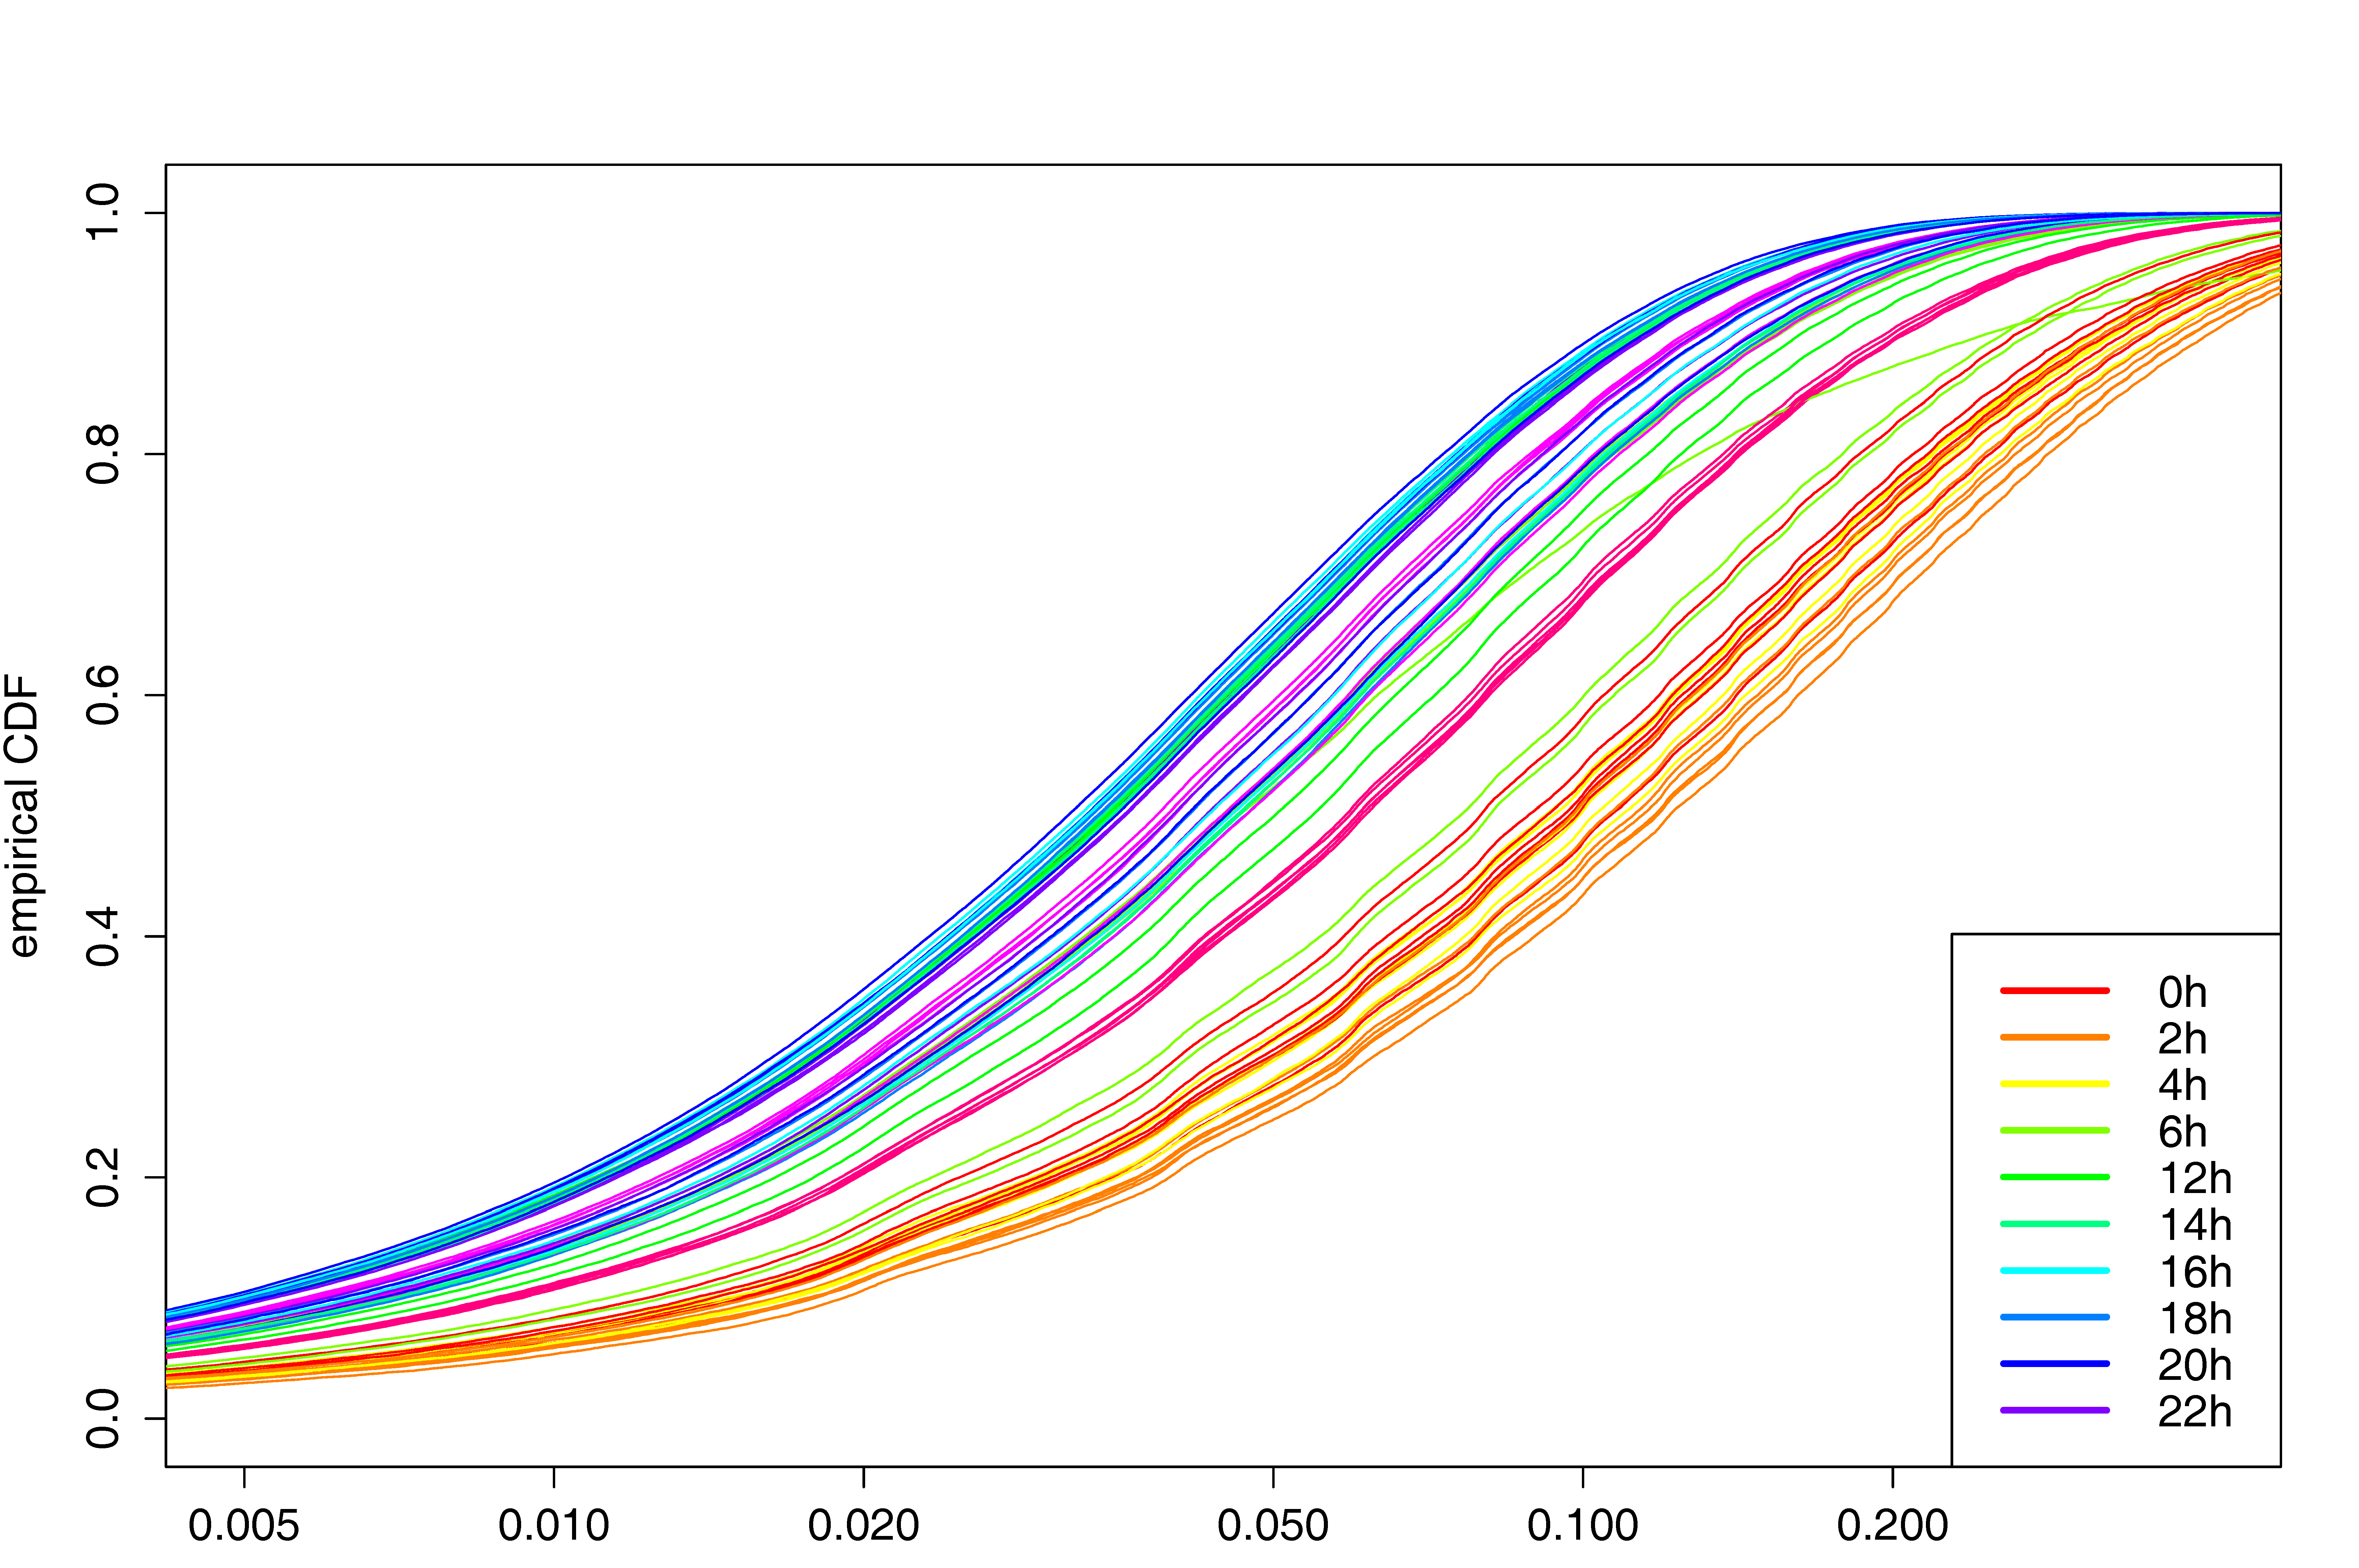
\includegraphics[width=\textwidth]{images/IMC2013/R-IAT-fromflows-umts-ecdfs-2h.png}
                \caption{Only UMTS tunnels with data flows.}
                \label{fig:IAT-ecdf-2h-active-umts}
        \end{subfigure}
        \caption{Empirical cumulative distribution function of the tunnel inter-arrival time in seconds by time of day for each day of one week.}\label{fig:IAT-ecdf-2h}
\end{figure}

To investigate the arrivals from yet another angle we take a look at inter-arrival time of the tunnels in Figure~\ref{fig:IAT-ecdf-2h}. This metric is more suited to describe the arrival process in the toy queuing model we propose. The empirical CDFs are again broken down by time of day, the same diurnal load oscillation can be observed. The medians range between about 20 and 60 milliseconds. Figure~\ref{fig:IAT-ecdf-2h-successful}, which represents all tunnel requests that the \ac{GGSN} successfully handled, shows wave-like steps in 20ms intervals in the plot. As this is happening very regularly at every time of the day we believe, that this effect must be from a source inside the mobile network and not induced from the outside, .e.g. through mobile devices.

This becomes even more peculiar when further breaking down the tunnel arrivals. We now distinguish between active tunnels, i.e. tunnels, that actually transported user traffic during their lifetime (cf. Fig.~\ref{fig:IAT-ecdf-2h-active}), and active tunnels, which were created while having a GPRS (Fig.~\ref{fig:IAT-ecdf-2h-active-gprs}) or UMTS (Fig.~\ref{fig:IAT-ecdf-2h-active-umts}) connectivity, respectively. Note that only about 86\% of requested and created tunnels where actually used for user data transmissions afterwards. The 20ms-steps occur strongest when observing all tunnel arrivals, in a weaker form it is also present in the active and \ac{UMTS} tunnel portion. 

Our working hypothesis as to the origin of the effect is the \ac{TTI}. This time indicates the duration of a radio transmission and is usually either 10 or 20 milliseconds in length. It is also in sync for the whole network of base stations making the \ac{TTI} noticeable even when not measuring directly at the radio link. The observed step-width of 20ms therefore indicates, that the signaling procedure the GTP CREATE is part of, includes at least one trip from the mobile device over the radio interface. This makes sense, as the tunnel is typically created during the GPRS Attach procedure, which is indeed initiated at the user's device. Unfortunately, this also makes the tunnel arrivals come in somewhat batched, which could momentarily increase the load at the \ac{GGSN} that then would need to process more requests at once than if the arrivals followed a smooth stochastic distribution.




%%%%%%%%%%%%%%%%%%%%%%%%%%%%%%%%%%%%%%%%%%%%%%%%%%%%%%%%%%%%%%%%%%%%%%%%%%%%%%%
\subsubsection{Tunnel Event Processing Time}

This brings us to another and potentially more direct measure of \ac{GGSN} load, namely the event processing time, meaning the time it takes for the \ac{GGSN} to fullfil a \ac{GTP} request. This is calculated from the requested and finished timestamps of every \ac{GTP} event in our dataset. As the measurement is conducted at the Gn interface these timestamps represent the time the \ac{GTP} signaling request moves to the \ac{GGSN} and the time the response transitions through the link.

As stated in the previous section, it would be of special interest to know if the setup time of tunnels is influenced by anything, as this is one of the \ac{GGSN}'s most time-sensitive jobs and can impact the time a user has to wait before being able to actually transfer data. Unfortunately, some issues with the dataset did not allow the investigation of the processing time of either create and delete messages.

\begin{figure}
	\centering
	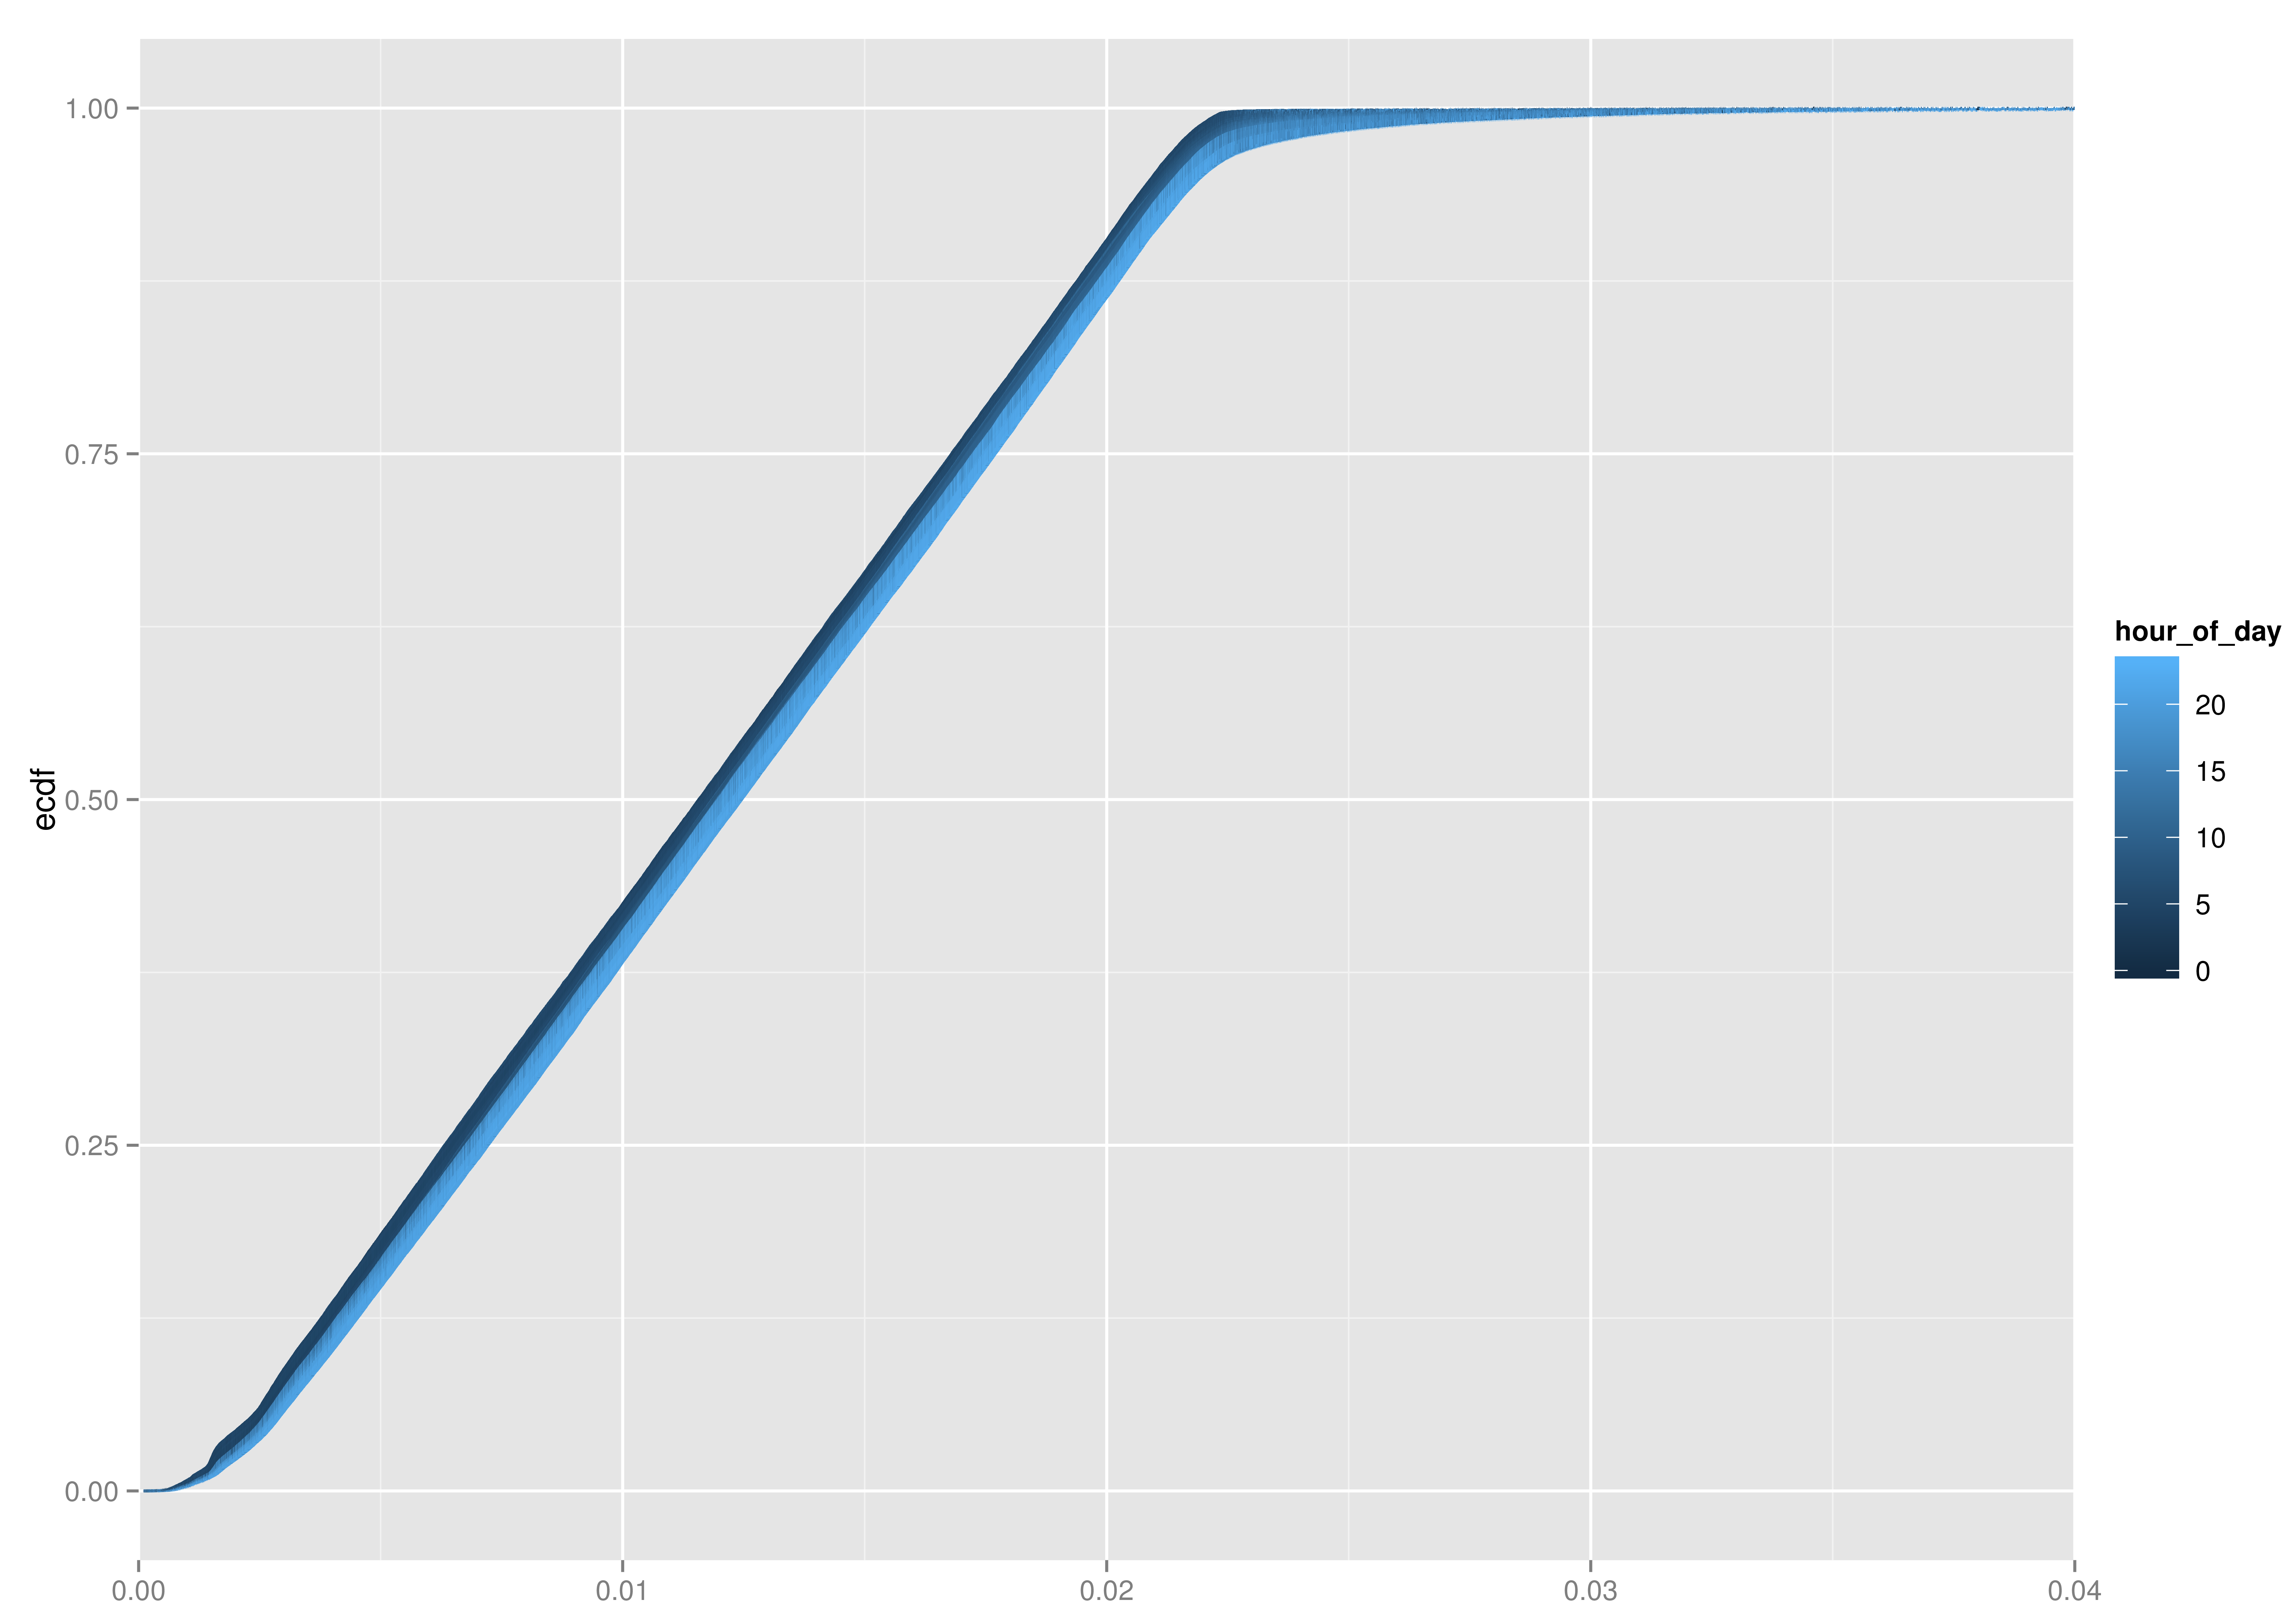
\includegraphics[width=\columnwidth]{images/IMC2013/R-update-time-cdfs.png}
	\caption{Empirical CDFs of the time it takes a GGSN to process a GTP update event, plotted for each hour of the day.}
	\label{fig:update-time}
\end{figure}


However, we could investigate the processing time of \ac{GTP} update messages. The core network transmits roughly two orders of magnitude more update than either create or delete events and therefore the number of usable events exceeded the significance level. While no direct investigation of the setup and deletion procedures was possible with these events, a rough overall picture of load can still be attained through this. Figure \ref{fig:update-time} depicts a band of empirical cumulative distribution functions for the processing time of update events broken down by time of day. The processing time is almost uniformly distributed between 2 and 22 milliseconds, with a slightly longer duration during the evening, making for a continuous uniform distribution. This is rather unexpected as uniform distributions do not usually occur in computing processes. According to the central limit theorem one would rather expect to see a normal distribution influenced by, e.g., scheduling or queuing artifacts. In the future we hope to investigate these features more closely, including a proper investigation of the tunnel setup and teardown processing time, if the dataset allows it.



%%%%%%%%%%%%%%%%%%%%%%%%%%%%%%%%%%%%%%%%%%%%%%%%%%%%%%%%%%%%%%%%%%%%%%%%%%%%%%%
%\paragraph{Relative Total Number of Tunnels in the Core}
%
% TODO: for the next paper?
%
%  tunnel numbers (relative?)
%  i.e. how much state is currently held in the core?




%!TEX root = paper.tex
%%%%%%%%%%%%%%%%%%%%%%%%%%%%%%%%%%%%%%%%%%%%%%%%%%%%%%%%%%%%%%%%%%%%%%%%%%%%%%%
\section{Load Modeling}
\label{sec:modeling-IMC}

Drawing conclusions from statistical analysis alone is a difficult task. The next logical step lies therefore in the creation of models abstracting this real system, making them easier to calculate with the loss of some precision. This and future improved models should support network operators in predicting the signaling load in their core network with the benefit of improved network engineering and correctly scaling core components.


%%%%%%%%%%%%%%%%%%%%%%%%%%%%%%%%%%%%%%%%%%%%%%%%%%%%%%%%%%%%%%%%%%%%%%%%%%%%%%%
\subsection{Creating a Simple Toy Queuing Model}

\begin{figure}
	\centering
	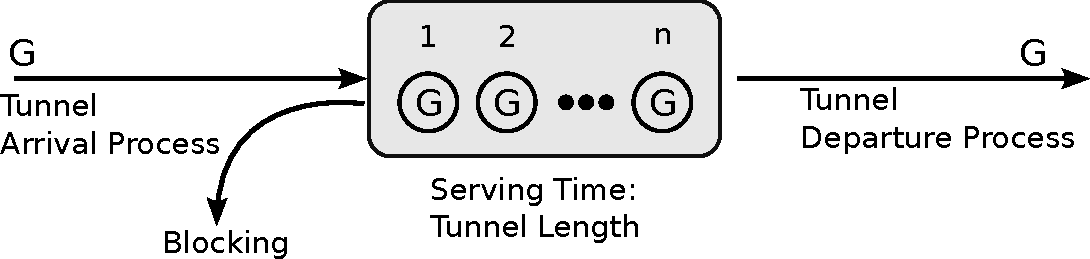
\includegraphics[width=\columnwidth]{images/IMC2013/GGn-model.pdf}
	\caption{Simple toy-model for tunnel-induced load on the core network.}
	\label{fig:ggn-model}
\end{figure}

To begin the modeling process we attempt to represent the tunnel management as a queuing system, specifically as a G/G/n-0 system in Kendall's notation. Figure~\ref{fig:ggn-model} shows this model for the case of our proposed tunnel load metric. Here, tunnels enter the system by a general random distribution, are then ``served'' at the \ac{GGSN} for the duration of their existence, which also follows a general distribution, and leave the system, i.e. are torn down, afterwards. If the serving units are filled, blocking occurs and arriving tunnel requests are rejected.

In this case ``servers'' correspond to available resources at one or more \ac{GGSN}, making the maximum number of tunnels hard to guess and depend on a number of factors. This could include soft-limits like the specific configuration, and hard-limits, e.g. the \ac{GGSN}'s processing and memory constraints. Unfortunately, all of these are unknown to us. Moreover, as the tunnels are all served on a relatively small number of hardware entities they are not independent of each other. Increasing load could very well influence both the arrival as well as the serving process.

For the purpose of creating a toy model we are further simplifying the G/G/n-0 to a M/M/$\infty$ queue. As stated, no actual limit to the number of virtual servers is known and the data also does not show any obvious limits. So we can safely assume an unlimited system and do not have to treat blocking or queuing explicitly.

\begin{figure}
	\centering
	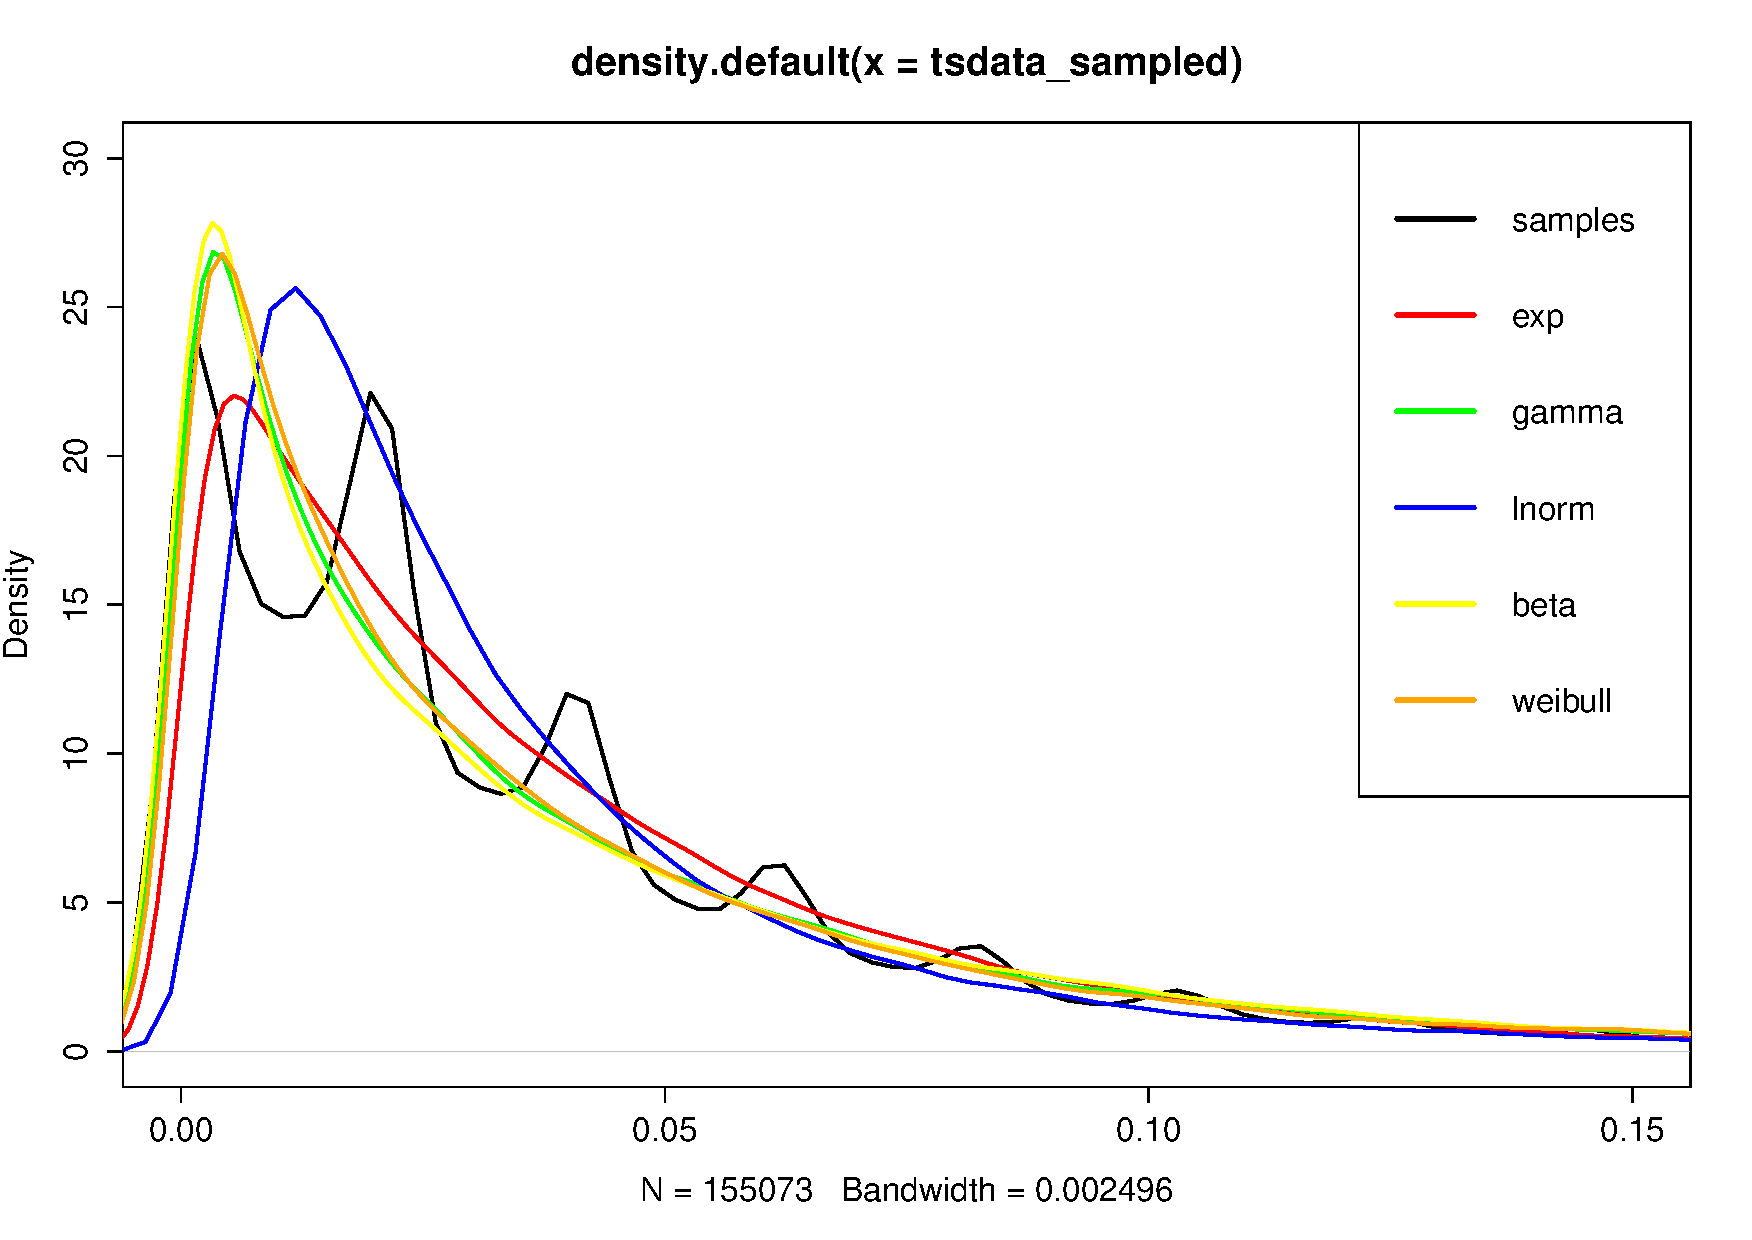
\includegraphics[width=\columnwidth]{images/IMC2013/R-IAT-densities.pdf}
	\caption{Sampled inter-arrival time density and fitted theoretical distributions.}
	\label{fig:IAT-densities}
\end{figure}

Furthermore, we fitted univariate distributions to the experimental data for the tunnel inter-arrivals and durations and tested the goodness of the fit both numerically, using Pearson's $\chi^2$ test, and visually for the density and CDF plots. No standard random distribution reaches the significance level for either process. We attribute this fact largely to the various artifacts in the data, e.g. the described wave effect every 20 milliseconds in the inter-arrival time. Matching them visually (confer also the density plot in Figure~\ref{fig:IAT-densities}) we find that the exponential fit is reasonably close to the experimental data in both the arrival and duration cases. Again, these distribution fits are just for a toy model to lay the groundwork for future and improved modeling.


\begin{figure}
	\centering
	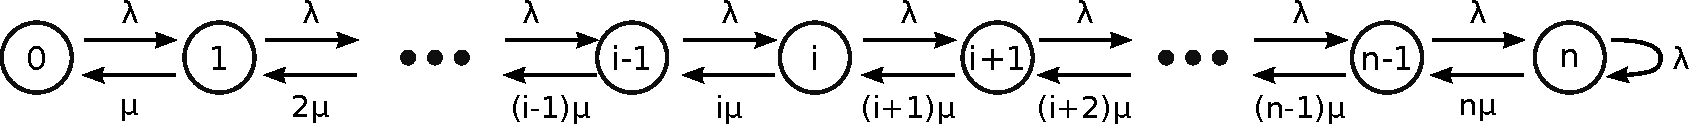
\includegraphics[width=\columnwidth]{images/IMC2013/markovchain.pdf}
	\caption{Markov chain model for the tunnel serving process.}
	\label{fig:markovchain}
\end{figure}

Now, assuming both a Poisson arrival and an exponential serving process, a Markov chain representing the queue can be set up (cf. Fig.~\ref{fig:markovchain}) and stationary analysis can be conducted. From the measured data an arrival rate of $\lambda=25.64123$ and the parameter $\mu=0.0001586728$ for the exponential service time distribution are calculated. Using Little's Law this gives an estimate for the mean number of concurrent tunnels at the \ac{GGSN} of 

$$
L=\frac{\lambda}{\mu}\approx 161\,599. %=161598.14.
$$

As stated, the amount of state held at the node and propagated through the network is directly related to the number of tunnels. Therefore, we propose this metric as an initial estimate of the load at the \ac{GGSN}. 


%%%%%%%%%%%%%%%%%%%%%%%%%%%%%%%%%%%%%%%%%%%%%%%%%%%%%%%%%%%%%%%%%%%%%%%%%%%%%%%
\subsection{Modeling Discussion}

On the basis of this toy model better fitting models can now be constructed. Those should also factor in more of the core network's properties and specified parameters omitted in this model. Specifically, this means shifting from M/M/$\infty$ to the more generalized G/G/n and therefore finding better distribution fits for the involved processes.

It is also entirely possible that the single queue approach is not the best way to describe control plane load. Several load influencing factors discussed earlier have direct influence on the tunnel arrivals and duration, e.g. the device type or the radio access technology. Therefore, amongst others multidimensional queuing networks or fluid flow could be a better fit. Our plan is to conduct further investigations into the modeling of mobile core network signaling. This also includes a rough simulative approach, which could also be used to validate our models against experimental data.




% \begin{figure}
% \centering
% 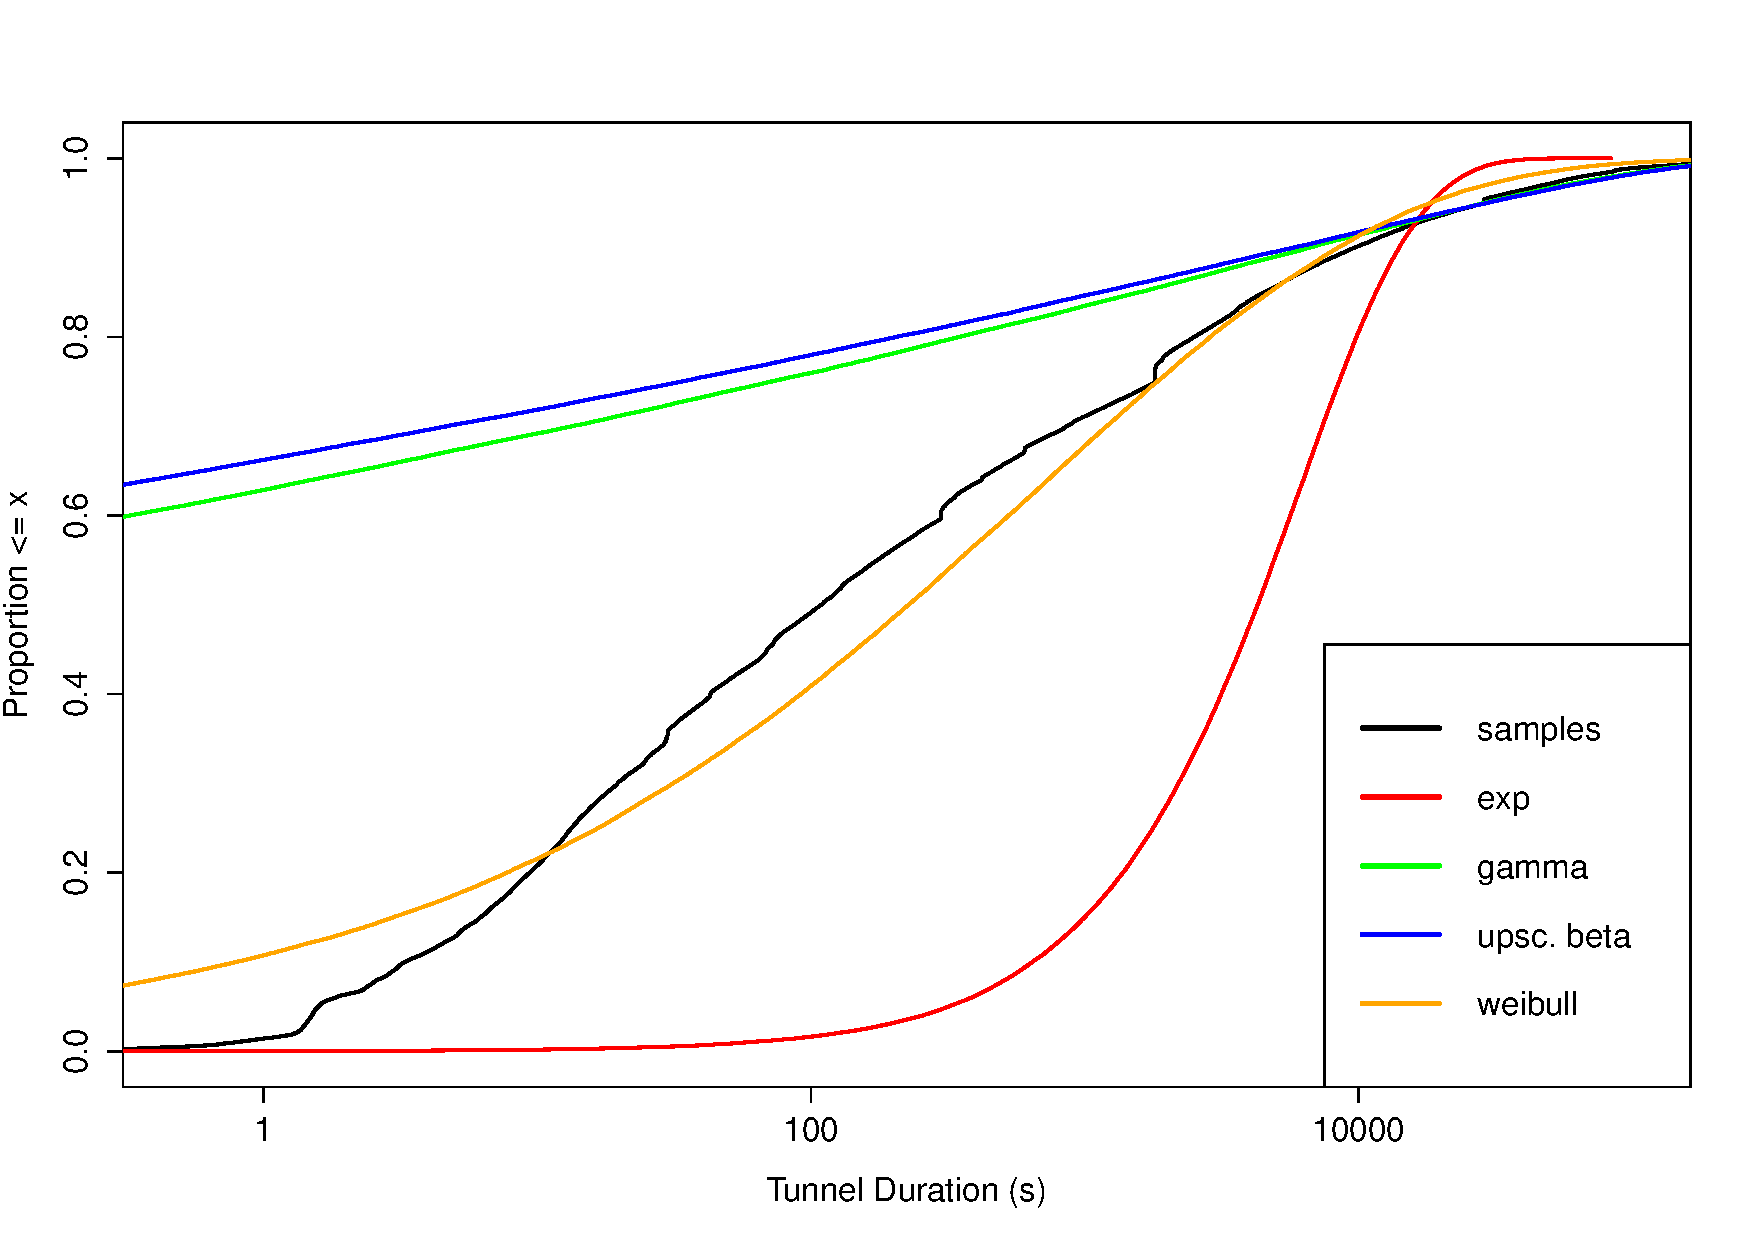
\includegraphics[width=\columnwidth]{figures/R-ST-ecdfs.pdf}
% \caption{Sampled serving time cumulative distribution function and fitted theoretical distributions.}
% \label{fig:ST-ecdf}
% \end{figure}

% \begin{figure}
% \centering
% 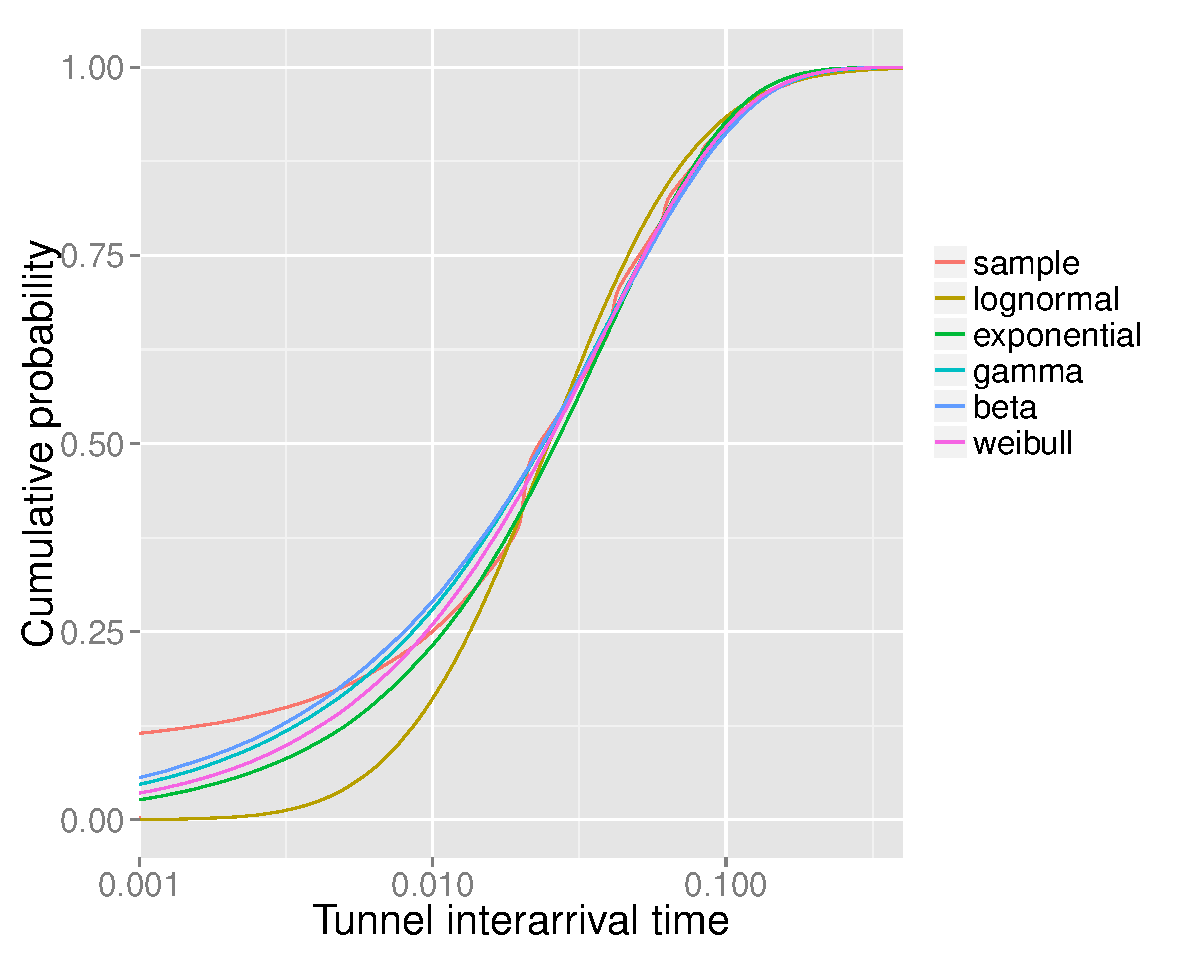
\includegraphics[width=\columnwidth]{figures/R-IAT-ecdfs.pdf}
% \caption{Sampled inter-arrival time cumulative distribution function and fitted theoretical distributions.}
% \label{fig:IAT-ecdfs}
% \end{figure}



%!TEX root = paper.tex
%%%%%%%%%%%%%%%%%%%%%%%%%%%%%%%%%%%%%%%%%%%%%%%%%%%%%%%%%%%%%%%%%%%%%%%%%%%%%%%
\section{Conclusion}
\label{sec:conclusion-IMC}
\acresetall

In this paper, we took a look at the signaling behavior of devices in an operational \ac{3G} mobile network providing Internet access. Our focus does not lie on the wireless or user-oriented parts of the network, but on signaling in the core network. To the best of our knowledge, this paper is the first to offer an in-depth core network perspective on signaling. We gave a \ac{GPRS} and \ac{UMTS} network primer, and introduced \ac{GTP} tunnel management and evaluated a week long data set recorded in the core network of an Austrian mobile operator.

In our observation of core network signaling involving \ac{PDP} Contexts and their management, we looked at the effect of device types and operating systems on the duration of \ac{GTP} tunnels. We can conclude that the distribution of tunnel durations in our evaluated dataset is dominated by smartphones. This is contrary to the conventional idea that a larger volume of user plane traffic also leads to an increase of signaling. In our dataset, this would mean that 3G dongles would cause most signaling, which is definitely not the case. Our paper shows that operators can determine which type of device has the most influence on the current network infrastructure by looking at and comparing tunnel duration distributions.

For additional load investigations we also looked at the inter-arrival and processing time of tunnels and found further evidence of radio and diurnal effects influencing the core network. With this data in mind, an initial M/M/$\infty$ queue was created to model load occurring at the \ac{GGSN} with simple stationary analysis. This also serves a basis for future more detailed models.

We think that this investigation and load modeling can lead to better network planning: Being more aware of the control plane provides the necessary tools to identify probable causes for control plane activity. We would also like to expand our evaluations, as there are several angles not investigated so far that could prove worthwhile. This includes an examination of the exact number and size of signaling messages flowing through the core, a more detailed picture of the processing load these messages induce at the \ac{GGSN}, and an evolved model. Furthermore, a differential analysis of our data compared to a newer dataset (potentially including \ac{LTE} access) could really prove worthwhile.

